\documentclass[twoside]{book}

% Packages required by doxygen
\usepackage{fixltx2e}
\usepackage{calc}
\usepackage{doxygen}
\usepackage[export]{adjustbox} % also loads graphicx
\usepackage{graphicx}
\usepackage[utf8]{inputenc}
\usepackage{makeidx}
\usepackage{multicol}
\usepackage{multirow}
\PassOptionsToPackage{warn}{textcomp}
\usepackage{textcomp}
\usepackage[nointegrals]{wasysym}
\usepackage[table]{xcolor}

% Font selection
\usepackage[T1]{fontenc}
\usepackage[scaled=.90]{helvet}
\usepackage{courier}
\usepackage{amssymb}
\usepackage{sectsty}
\renewcommand{\familydefault}{\sfdefault}
\allsectionsfont{%
  \fontseries{bc}\selectfont%
  \color{darkgray}%
}
\renewcommand{\DoxyLabelFont}{%
  \fontseries{bc}\selectfont%
  \color{darkgray}%
}
\newcommand{\+}{\discretionary{\mbox{\scriptsize$\hookleftarrow$}}{}{}}

% Page & text layout
\usepackage{geometry}
\geometry{%
  a4paper,%
  top=2.5cm,%
  bottom=2.5cm,%
  left=2.5cm,%
  right=2.5cm%
}
\tolerance=750
\hfuzz=15pt
\hbadness=750
\setlength{\emergencystretch}{15pt}
\setlength{\parindent}{0cm}
\setlength{\parskip}{3ex plus 2ex minus 2ex}
\makeatletter
\renewcommand{\paragraph}{%
  \@startsection{paragraph}{4}{0ex}{-1.0ex}{1.0ex}{%
    \normalfont\normalsize\bfseries\SS@parafont%
  }%
}
\renewcommand{\subparagraph}{%
  \@startsection{subparagraph}{5}{0ex}{-1.0ex}{1.0ex}{%
    \normalfont\normalsize\bfseries\SS@subparafont%
  }%
}
\makeatother

% Headers & footers
\usepackage{fancyhdr}
\pagestyle{fancyplain}
\fancyhead[LE]{\fancyplain{}{\bfseries\thepage}}
\fancyhead[CE]{\fancyplain{}{}}
\fancyhead[RE]{\fancyplain{}{\bfseries\leftmark}}
\fancyhead[LO]{\fancyplain{}{\bfseries\rightmark}}
\fancyhead[CO]{\fancyplain{}{}}
\fancyhead[RO]{\fancyplain{}{\bfseries\thepage}}
\fancyfoot[LE]{\fancyplain{}{}}
\fancyfoot[CE]{\fancyplain{}{}}
\fancyfoot[RE]{\fancyplain{}{\bfseries\scriptsize Generated by Doxygen }}
\fancyfoot[LO]{\fancyplain{}{\bfseries\scriptsize Generated by Doxygen }}
\fancyfoot[CO]{\fancyplain{}{}}
\fancyfoot[RO]{\fancyplain{}{}}
\renewcommand{\footrulewidth}{0.4pt}
\renewcommand{\chaptermark}[1]{%
  \markboth{#1}{}%
}
\renewcommand{\sectionmark}[1]{%
  \markright{\thesection\ #1}%
}

% Indices & bibliography
\usepackage{natbib}
\usepackage[titles]{tocloft}
\setcounter{tocdepth}{3}
\setcounter{secnumdepth}{5}
\makeindex

% Hyperlinks (required, but should be loaded last)
\usepackage{ifpdf}
\ifpdf
  \usepackage[pdftex,pagebackref=true]{hyperref}
\else
  \usepackage[ps2pdf,pagebackref=true]{hyperref}
\fi
\hypersetup{%
  colorlinks=true,%
  linkcolor=blue,%
  citecolor=blue,%
  unicode%
}

% Custom commands
\newcommand{\clearemptydoublepage}{%
  \newpage{\pagestyle{empty}\cleardoublepage}%
}

\usepackage{caption}
\captionsetup{labelsep=space,justification=centering,font={bf},singlelinecheck=off,skip=4pt,position=top}

%===== C O N T E N T S =====

\begin{document}

% Titlepage & ToC
\hypersetup{pageanchor=false,
             bookmarksnumbered=true,
             pdfencoding=unicode
            }
\pagenumbering{alph}
\begin{titlepage}
\vspace*{7cm}
\begin{center}%
{\Large Rhino\+X-\/\+S\+DK }\\
\vspace*{1cm}
{\large Generated by Doxygen 1.8.14}\\
\end{center}
\end{titlepage}
\clearemptydoublepage
\pagenumbering{roman}
\tableofcontents
\clearemptydoublepage
\pagenumbering{arabic}
\hypersetup{pageanchor=true}

%--- Begin generated contents ---
\chapter{Namespace Index}
\section{Namespace List}
Here is a list of all documented namespaces with brief descriptions\+:\begin{DoxyCompactList}
\item\contentsline{section}{\mbox{\hyperlink{namespace_ximmerse}{Ximmerse}} }{\pageref{namespace_ximmerse}}{}
\item\contentsline{section}{\mbox{\hyperlink{namespace_ximmerse_1_1_rhino_x}{Ximmerse.\+RhinoX}} }{\pageref{namespace_ximmerse_1_1_rhino_x}}{}
\item\contentsline{section}{\mbox{\hyperlink{namespace_ximmerse_1_1_rhino_x_1_1_internal}{Ximmerse.\+Rhino\+X.\+Internal}} }{\pageref{namespace_ximmerse_1_1_rhino_x_1_1_internal}}{}
\end{DoxyCompactList}

\chapter{Hierarchical Index}
\section{Class Hierarchy}
This inheritance list is sorted roughly, but not completely, alphabetically\+:\begin{DoxyCompactList}
\item \contentsline{section}{Ximmerse.\+Rhino\+X.\+A\+I\+O\+Event}{\pageref{struct_ximmerse_1_1_rhino_x_1_1_a_i_o_event}}{}
\item Base\+Input\+Module\begin{DoxyCompactList}
\item \contentsline{section}{Ximmerse.\+Rhino\+X.\+R\+X\+Input\+Module}{\pageref{class_ximmerse_1_1_rhino_x_1_1_r_x_input_module}}{}
\end{DoxyCompactList}
\item Base\+Raycaster\begin{DoxyCompactList}
\item \contentsline{section}{Ximmerse.\+Rhino\+X.\+R\+X\+Raycaster}{\pageref{class_ximmerse_1_1_rhino_x_1_1_r_x_raycaster}}{}
\end{DoxyCompactList}
\item \contentsline{section}{Ximmerse.\+Rhino\+X.\+Calibration\+Serialization\+Data}{\pageref{class_ximmerse_1_1_rhino_x_1_1_calibration_serialization_data}}{}
\item \contentsline{section}{Ximmerse.\+Rhino\+X.\+Tracked\+Object\+Json.\+Card\+Group\+Json}{\pageref{class_ximmerse_1_1_rhino_x_1_1_tracked_object_json_1_1_card_group_json}}{}
\item \contentsline{section}{Ximmerse.\+Rhino\+X.\+Controller\+Gyroscope}{\pageref{struct_ximmerse_1_1_rhino_x_1_1_controller_gyroscope}}{}
\item Event\+System\begin{DoxyCompactList}
\item \contentsline{section}{Ximmerse.\+Rhino\+X.\+R\+X\+Event\+System}{\pageref{class_ximmerse_1_1_rhino_x_1_1_r_x_event_system}}{}
\end{DoxyCompactList}
\item Mono\+Behaviour\begin{DoxyCompactList}
\item \contentsline{section}{Ximmerse.\+Rhino\+X.\+A\+R\+Camera}{\pageref{class_ximmerse_1_1_rhino_x_1_1_a_r_camera}}{}
\item \contentsline{section}{Ximmerse.\+Rhino\+X.\+Composite\+Ground\+Plane}{\pageref{class_ximmerse_1_1_rhino_x_1_1_composite_ground_plane}}{}
\item \contentsline{section}{Ximmerse.\+Rhino\+X.\+Dynamic\+Target}{\pageref{class_ximmerse_1_1_rhino_x_1_1_dynamic_target}}{}
\item \contentsline{section}{Ximmerse.\+Rhino\+X.\+Ground\+Plane}{\pageref{class_ximmerse_1_1_rhino_x_1_1_ground_plane}}{}
\item \contentsline{section}{Ximmerse.\+Rhino\+X.\+Overlay}{\pageref{class_ximmerse_1_1_rhino_x_1_1_overlay}}{}
\item \contentsline{section}{Ximmerse.\+Rhino\+X.\+Runtime\+Calibration\+Entity}{\pageref{class_ximmerse_1_1_rhino_x_1_1_runtime_calibration_entity}}{}
\item \contentsline{section}{Ximmerse.\+Rhino\+X.\+Runtime\+Calibration\+Manager}{\pageref{class_ximmerse_1_1_rhino_x_1_1_runtime_calibration_manager}}{}
\item \contentsline{section}{Ximmerse.\+Rhino\+X.\+R\+X\+Controller}{\pageref{class_ximmerse_1_1_rhino_x_1_1_r_x_controller}}{}
\item \contentsline{section}{Ximmerse.\+Rhino\+X.\+Trackable\+Identity}{\pageref{class_ximmerse_1_1_rhino_x_1_1_trackable_identity}}{}
\end{DoxyCompactList}
\item \contentsline{section}{Ximmerse.\+Rhino\+X.\+Pose}{\pageref{struct_ximmerse_1_1_rhino_x_1_1_pose}}{}
\item Scriptable\+Object\begin{DoxyCompactList}
\item \contentsline{section}{Ximmerse.\+Rhino\+X.\+Object\+Tracking\+Profile}{\pageref{class_ximmerse_1_1_rhino_x_1_1_object_tracking_profile}}{}
\end{DoxyCompactList}
\item \contentsline{section}{Ximmerse.\+Rhino\+X.\+S\+D\+K\+Version}{\pageref{struct_ximmerse_1_1_rhino_x_1_1_s_d_k_version}}{}
\item \contentsline{section}{Ximmerse.\+Rhino\+X.\+Tracked\+Object\+Json.\+Single\+Card\+Json}{\pageref{class_ximmerse_1_1_rhino_x_1_1_tracked_object_json_1_1_single_card_json}}{}
\item \contentsline{section}{Ximmerse.\+Rhino\+X.\+Tracked\+Object\+Json}{\pageref{class_ximmerse_1_1_rhino_x_1_1_tracked_object_json}}{}
\item \contentsline{section}{Ximmerse.\+Rhino\+X.\+Object\+Tracking\+Profile.\+Tracking\+Items}{\pageref{class_ximmerse_1_1_rhino_x_1_1_object_tracking_profile_1_1_tracking_items}}{}
\item Unity\+Event\begin{DoxyCompactList}
\item \contentsline{section}{Ximmerse.\+Rhino\+X.\+Visiblity\+Change\+Event}{\pageref{class_ximmerse_1_1_rhino_x_1_1_visiblity_change_event}}{}
\end{DoxyCompactList}
\item Unity\+Event\begin{DoxyCompactList}
\item \contentsline{section}{Ximmerse.\+Rhino\+X.\+R\+X\+Controller.\+Controller\+Button\+Event}{\pageref{class_ximmerse_1_1_rhino_x_1_1_r_x_controller_1_1_controller_button_event}}{}
\end{DoxyCompactList}
\end{DoxyCompactList}

\chapter{Class Index}
\section{Class List}
Here are the classes, structs, unions and interfaces with brief descriptions\+:\begin{DoxyCompactList}
\item\contentsline{section}{\mbox{\hyperlink{struct_ximmerse_1_1_rhino_x_1_1_a_i_o_event}{Ximmerse.\+Rhino\+X.\+A\+I\+O\+Event}} \\*A\+IO event \+: device status event. Application may catch this event for device management. }{\pageref{struct_ximmerse_1_1_rhino_x_1_1_a_i_o_event}}{}
\item\contentsline{section}{\mbox{\hyperlink{class_ximmerse_1_1_rhino_x_1_1_a_r_camera}{Ximmerse.\+Rhino\+X.\+A\+R\+Camera}} \\*AR camera is the script that represents virtual camera in AR world. Developer may get the position/rotation of current head transform. }{\pageref{class_ximmerse_1_1_rhino_x_1_1_a_r_camera}}{}
\item\contentsline{section}{\mbox{\hyperlink{class_ximmerse_1_1_rhino_x_1_1_calibration_serialization_data}{Ximmerse.\+Rhino\+X.\+Calibration\+Serialization\+Data}} \\*Calibration serialization data. 用于持久化的数据格式。 }{\pageref{class_ximmerse_1_1_rhino_x_1_1_calibration_serialization_data}}{}
\item\contentsline{section}{\mbox{\hyperlink{class_ximmerse_1_1_rhino_x_1_1_tracked_object_json_1_1_card_group_json}{Ximmerse.\+Rhino\+X.\+Tracked\+Object\+Json.\+Card\+Group\+Json}} }{\pageref{class_ximmerse_1_1_rhino_x_1_1_tracked_object_json_1_1_card_group_json}}{}
\item\contentsline{section}{\mbox{\hyperlink{class_ximmerse_1_1_rhino_x_1_1_composite_ground_plane}{Ximmerse.\+Rhino\+X.\+Composite\+Ground\+Plane}} \\*Composite ground plane \+: composite of multiple ground plane to align the head pose. Composite ground plane should be singleton in your scene. }{\pageref{class_ximmerse_1_1_rhino_x_1_1_composite_ground_plane}}{}
\item\contentsline{section}{\mbox{\hyperlink{class_ximmerse_1_1_rhino_x_1_1_r_x_controller_1_1_controller_button_event}{Ximmerse.\+Rhino\+X.\+R\+X\+Controller.\+Controller\+Button\+Event}} }{\pageref{class_ximmerse_1_1_rhino_x_1_1_r_x_controller_1_1_controller_button_event}}{}
\item\contentsline{section}{\mbox{\hyperlink{struct_ximmerse_1_1_rhino_x_1_1_controller_gyroscope}{Ximmerse.\+Rhino\+X.\+Controller\+Gyroscope}} \\*Controller gyroscope information }{\pageref{struct_ximmerse_1_1_rhino_x_1_1_controller_gyroscope}}{}
\item\contentsline{section}{\mbox{\hyperlink{class_ximmerse_1_1_rhino_x_1_1_dynamic_target}{Ximmerse.\+Rhino\+X.\+Dynamic\+Target}} \\*Default trackable behaviour, updates trackable object\textquotesingle{}s transform at the head space per-\/frame. }{\pageref{class_ximmerse_1_1_rhino_x_1_1_dynamic_target}}{}
\item\contentsline{section}{\mbox{\hyperlink{class_ximmerse_1_1_rhino_x_1_1_ground_plane}{Ximmerse.\+Rhino\+X.\+Ground\+Plane}} \\*Ground plane represents static trackable object placed on environment, to reposition head pose according to the relative pose between head and trackable object. }{\pageref{class_ximmerse_1_1_rhino_x_1_1_ground_plane}}{}
\item\contentsline{section}{\mbox{\hyperlink{class_ximmerse_1_1_rhino_x_1_1_object_tracking_profile}{Ximmerse.\+Rhino\+X.\+Object\+Tracking\+Profile}} }{\pageref{class_ximmerse_1_1_rhino_x_1_1_object_tracking_profile}}{}
\item\contentsline{section}{\mbox{\hyperlink{class_ximmerse_1_1_rhino_x_1_1_overlay}{Ximmerse.\+Rhino\+X.\+Overlay}} \\*\mbox{\hyperlink{class_ximmerse_1_1_rhino_x_1_1_overlay}{Overlay}} \+: scripts for overlay rendering. }{\pageref{class_ximmerse_1_1_rhino_x_1_1_overlay}}{}
\item\contentsline{section}{\mbox{\hyperlink{struct_ximmerse_1_1_rhino_x_1_1_pose}{Ximmerse.\+Rhino\+X.\+Pose}} \\*Structure \+: position, rotation and time stamp. }{\pageref{struct_ximmerse_1_1_rhino_x_1_1_pose}}{}
\item\contentsline{section}{\mbox{\hyperlink{class_ximmerse_1_1_rhino_x_1_1_runtime_calibration_entity}{Ximmerse.\+Rhino\+X.\+Runtime\+Calibration\+Entity}} \\*Runtime calibration entry. }{\pageref{class_ximmerse_1_1_rhino_x_1_1_runtime_calibration_entity}}{}
\item\contentsline{section}{\mbox{\hyperlink{class_ximmerse_1_1_rhino_x_1_1_runtime_calibration_manager}{Ximmerse.\+Rhino\+X.\+Runtime\+Calibration\+Manager}} \\*Runtime calibration manager. }{\pageref{class_ximmerse_1_1_rhino_x_1_1_runtime_calibration_manager}}{}
\item\contentsline{section}{\mbox{\hyperlink{class_ximmerse_1_1_rhino_x_1_1_r_x_controller}{Ximmerse.\+Rhino\+X.\+R\+X\+Controller}} \\*High level S\+DK script for developers to access controller data and event, e.\+g. buttons, gyroscopes, finger point over touch-\/pad. }{\pageref{class_ximmerse_1_1_rhino_x_1_1_r_x_controller}}{}
\item\contentsline{section}{\mbox{\hyperlink{class_ximmerse_1_1_rhino_x_1_1_r_x_event_system}{Ximmerse.\+Rhino\+X.\+R\+X\+Event\+System}} \\*\mbox{\hyperlink{namespace_ximmerse_1_1_rhino_x}{RhinoX}} event system, should be singleton instance, driver class of \mbox{\hyperlink{namespace_ximmerse_1_1_rhino_x}{RhinoX}} input event system. Note\+: \mbox{\hyperlink{class_ximmerse_1_1_rhino_x_1_1_r_x_event_system}{R\+X\+Event\+System}} need to be the only event system, if your scene has Unity\textquotesingle{}s built in Event\+System instane, \mbox{\hyperlink{class_ximmerse_1_1_rhino_x_1_1_r_x_event_system}{R\+X\+Event\+System}} will remove it when starts. }{\pageref{class_ximmerse_1_1_rhino_x_1_1_r_x_event_system}}{}
\item\contentsline{section}{\mbox{\hyperlink{class_ximmerse_1_1_rhino_x_1_1_r_x_input_module}{Ximmerse.\+Rhino\+X.\+R\+X\+Input\+Module}} \\*\mbox{\hyperlink{namespace_ximmerse_1_1_rhino_x}{RhinoX}} controller module, public interface to ximmerse controller input event system. }{\pageref{class_ximmerse_1_1_rhino_x_1_1_r_x_input_module}}{}
\item\contentsline{section}{\mbox{\hyperlink{class_ximmerse_1_1_rhino_x_1_1_r_x_raycaster}{Ximmerse.\+Rhino\+X.\+R\+X\+Raycaster}} \\*Rhino-\/X raycaster. }{\pageref{class_ximmerse_1_1_rhino_x_1_1_r_x_raycaster}}{}
\item\contentsline{section}{\mbox{\hyperlink{struct_ximmerse_1_1_rhino_x_1_1_s_d_k_version}{Ximmerse.\+Rhino\+X.\+S\+D\+K\+Version}} \\*S\+DK version. }{\pageref{struct_ximmerse_1_1_rhino_x_1_1_s_d_k_version}}{}
\item\contentsline{section}{\mbox{\hyperlink{class_ximmerse_1_1_rhino_x_1_1_tracked_object_json_1_1_single_card_json}{Ximmerse.\+Rhino\+X.\+Tracked\+Object\+Json.\+Single\+Card\+Json}} }{\pageref{class_ximmerse_1_1_rhino_x_1_1_tracked_object_json_1_1_single_card_json}}{}
\item\contentsline{section}{\mbox{\hyperlink{class_ximmerse_1_1_rhino_x_1_1_trackable_identity}{Ximmerse.\+Rhino\+X.\+Trackable\+Identity}} \\*Trackable object identity. Constraint by an integral trackable ID , represents a trackable object in real world. }{\pageref{class_ximmerse_1_1_rhino_x_1_1_trackable_identity}}{}
\item\contentsline{section}{\mbox{\hyperlink{class_ximmerse_1_1_rhino_x_1_1_tracked_object_json}{Ximmerse.\+Rhino\+X.\+Tracked\+Object\+Json}} \\*Tracked object json. }{\pageref{class_ximmerse_1_1_rhino_x_1_1_tracked_object_json}}{}
\item\contentsline{section}{\mbox{\hyperlink{class_ximmerse_1_1_rhino_x_1_1_object_tracking_profile_1_1_tracking_items}{Ximmerse.\+Rhino\+X.\+Object\+Tracking\+Profile.\+Tracking\+Items}} }{\pageref{class_ximmerse_1_1_rhino_x_1_1_object_tracking_profile_1_1_tracking_items}}{}
\item\contentsline{section}{\mbox{\hyperlink{class_ximmerse_1_1_rhino_x_1_1_triple_ground_plane}{Ximmerse.\+Rhino\+X.\+Triple\+Ground\+Plane}} \\*Tripple ground plane. }{\pageref{class_ximmerse_1_1_rhino_x_1_1_triple_ground_plane}}{}
\item\contentsline{section}{\mbox{\hyperlink{class_ximmerse_1_1_rhino_x_1_1_visiblity_change_event}{Ximmerse.\+Rhino\+X.\+Visiblity\+Change\+Event}} }{\pageref{class_ximmerse_1_1_rhino_x_1_1_visiblity_change_event}}{}
\end{DoxyCompactList}

\chapter{Namespace Documentation}
\hypertarget{namespace_ximmerse}{}\section{Ximmerse Namespace Reference}
\label{namespace_ximmerse}\index{Ximmerse@{Ximmerse}}
\subsection*{Namespaces}
\begin{DoxyCompactItemize}
\end{DoxyCompactItemize}

\hypertarget{namespace_ximmerse_1_1_rhino_x}{}\section{Ximmerse.\+RhinoX Namespace Reference}
\label{namespace_ximmerse_1_1_rhino_x}\index{Ximmerse.\+RhinoX@{Ximmerse.\+RhinoX}}
\subsection*{Namespaces}
\begin{DoxyCompactItemize}
\end{DoxyCompactItemize}
\subsection*{Classes}
\begin{DoxyCompactItemize}
\item 
struct \mbox{\hyperlink{struct_ximmerse_1_1_rhino_x_1_1_a_i_o_event}{A\+I\+O\+Event}}
\begin{DoxyCompactList}\small\item\em A\+IO event \+: device status event. Application may catch this event for device management. \end{DoxyCompactList}\item 
class {\bfseries A\+I\+O\+System}
\begin{DoxyCompactList}\small\item\em A\+IO system \+: access system software and hardware information. \end{DoxyCompactList}\item 
class \mbox{\hyperlink{class_ximmerse_1_1_rhino_x_1_1_a_r_camera}{A\+R\+Camera}}
\begin{DoxyCompactList}\small\item\em AR camera is the script that represents virtual camera in AR world. Developer may get the position/rotation of current head transform. \end{DoxyCompactList}\item 
struct {\bfseries Calibrate\+Result}
\begin{DoxyCompactList}\small\item\em Calibrate result. \end{DoxyCompactList}\item 
class \mbox{\hyperlink{class_ximmerse_1_1_rhino_x_1_1_calibration_serialization_data}{Calibration\+Serialization\+Data}}
\begin{DoxyCompactList}\small\item\em Calibration serialization data. 用于持久化的数据格式。 \end{DoxyCompactList}\item 
class \mbox{\hyperlink{class_ximmerse_1_1_rhino_x_1_1_composite_ground_plane}{Composite\+Ground\+Plane}}
\begin{DoxyCompactList}\small\item\em Composite ground plane \+: composite of multiple ground plane to align the head pose. Composite ground plane should be singleton in your scene. \end{DoxyCompactList}\item 
struct \mbox{\hyperlink{struct_ximmerse_1_1_rhino_x_1_1_controller_gyroscope}{Controller\+Gyroscope}}
\begin{DoxyCompactList}\small\item\em Controller gyroscope information \end{DoxyCompactList}\item 
class \mbox{\hyperlink{class_ximmerse_1_1_rhino_x_1_1_dynamic_target}{Dynamic\+Target}}
\begin{DoxyCompactList}\small\item\em Default trackable behaviour, updates trackable object\textquotesingle{}s transform at the head space per-\/frame. \end{DoxyCompactList}\item 
class \mbox{\hyperlink{class_ximmerse_1_1_rhino_x_1_1_ground_plane}{Ground\+Plane}}
\begin{DoxyCompactList}\small\item\em Ground plane represents static trackable object placed on environment, to reposition head pose according to the relative pose between head and trackable object. \end{DoxyCompactList}\item 
struct {\bfseries Marker\+Config\+Info}
\begin{DoxyCompactList}\small\item\em Marker config info \+: a single marker object\textquotesingle{}s config info from J\+S\+ON. \end{DoxyCompactList}\item 
class {\bfseries Object\+Tracking}
\begin{DoxyCompactList}\small\item\em Object tracking \+: access tag tracking interface. \end{DoxyCompactList}\item 
class \mbox{\hyperlink{class_ximmerse_1_1_rhino_x_1_1_object_tracking_profile}{Object\+Tracking\+Profile}}
\item 
class \mbox{\hyperlink{class_ximmerse_1_1_rhino_x_1_1_overlay}{Overlay}}
\begin{DoxyCompactList}\small\item\em \mbox{\hyperlink{class_ximmerse_1_1_rhino_x_1_1_overlay}{Overlay}} \+: scripts for overlay rendering. \end{DoxyCompactList}\item 
struct \mbox{\hyperlink{struct_ximmerse_1_1_rhino_x_1_1_pose}{Pose}}
\begin{DoxyCompactList}\small\item\em Structure \+: position, rotation and time stamp. \end{DoxyCompactList}\item 
class \mbox{\hyperlink{class_ximmerse_1_1_rhino_x_1_1_runtime_calibration_entity}{Runtime\+Calibration\+Entity}}
\begin{DoxyCompactList}\small\item\em Runtime calibration entry. \end{DoxyCompactList}\item 
class \mbox{\hyperlink{class_ximmerse_1_1_rhino_x_1_1_runtime_calibration_manager}{Runtime\+Calibration\+Manager}}
\begin{DoxyCompactList}\small\item\em Runtime calibration manager. \end{DoxyCompactList}\item 
class \mbox{\hyperlink{class_ximmerse_1_1_rhino_x_1_1_r_x_controller}{R\+X\+Controller}}
\begin{DoxyCompactList}\small\item\em High level S\+DK script for developers to access controller data and event, e.\+g. buttons, gyroscopes, finger point over touch-\/pad. \end{DoxyCompactList}\item 
class \mbox{\hyperlink{class_ximmerse_1_1_rhino_x_1_1_r_x_event_system}{R\+X\+Event\+System}}
\begin{DoxyCompactList}\small\item\em \mbox{\hyperlink{namespace_ximmerse_1_1_rhino_x}{RhinoX}} event system, should be singleton instance, driver class of \mbox{\hyperlink{namespace_ximmerse_1_1_rhino_x}{RhinoX}} input event system. Note\+: \mbox{\hyperlink{class_ximmerse_1_1_rhino_x_1_1_r_x_event_system}{R\+X\+Event\+System}} need to be the only event system, if your scene has Unity\textquotesingle{}s built in Event\+System instane, \mbox{\hyperlink{class_ximmerse_1_1_rhino_x_1_1_r_x_event_system}{R\+X\+Event\+System}} will remove it when starts. \end{DoxyCompactList}\item 
class \mbox{\hyperlink{class_ximmerse_1_1_rhino_x_1_1_r_x_input_module}{R\+X\+Input\+Module}}
\begin{DoxyCompactList}\small\item\em \mbox{\hyperlink{namespace_ximmerse_1_1_rhino_x}{RhinoX}} controller module, public interface to ximmerse controller input event system. \end{DoxyCompactList}\item 
class \mbox{\hyperlink{class_ximmerse_1_1_rhino_x_1_1_r_x_raycaster}{R\+X\+Raycaster}}
\begin{DoxyCompactList}\small\item\em Rhino-\/X raycaster. \end{DoxyCompactList}\item 
class {\bfseries R\+X\+Raycast\+Info}
\begin{DoxyCompactList}\small\item\em \mbox{\hyperlink{namespace_ximmerse_1_1_rhino_x_1_1_internal}{Internal}} struct for rx-\/raycaster info \end{DoxyCompactList}\item 
struct \mbox{\hyperlink{struct_ximmerse_1_1_rhino_x_1_1_s_d_k_version}{S\+D\+K\+Version}}
\begin{DoxyCompactList}\small\item\em S\+DK version. \end{DoxyCompactList}\item 
class \mbox{\hyperlink{class_ximmerse_1_1_rhino_x_1_1_trackable_identity}{Trackable\+Identity}}
\begin{DoxyCompactList}\small\item\em Trackable object identity. Constraint by an integral trackable ID , represents a trackable object in real world. \end{DoxyCompactList}\item 
class \mbox{\hyperlink{class_ximmerse_1_1_rhino_x_1_1_tracked_object_json}{Tracked\+Object\+Json}}
\begin{DoxyCompactList}\small\item\em Tracked object json. \end{DoxyCompactList}\item 
class \mbox{\hyperlink{class_ximmerse_1_1_rhino_x_1_1_triple_ground_plane}{Triple\+Ground\+Plane}}
\begin{DoxyCompactList}\small\item\em Tripple ground plane. \end{DoxyCompactList}\item 
class \mbox{\hyperlink{class_ximmerse_1_1_rhino_x_1_1_visiblity_change_event}{Visiblity\+Change\+Event}}
\item 
class {\bfseries Ximmerse\+Controller\+System}
\begin{DoxyCompactList}\small\item\em Script to access \mbox{\hyperlink{namespace_ximmerse}{Ximmerse}} controller interfaces. \end{DoxyCompactList}\end{DoxyCompactItemize}
\subsection*{Enumerations}
\begin{DoxyCompactItemize}
\item 
enum \mbox{\hyperlink{namespace_ximmerse_1_1_rhino_x_ab081ae2f0ca6ea05a0a1ab6143ba91a1}{A\+I\+O\+Event\+Type}} \{ \newline
{\bfseries k\+Event\+None} = 0, 
{\bfseries k\+Event\+Sdk\+Service\+Starting} = 1, 
{\bfseries k\+Event\+Sdk\+Service\+Started} = 2, 
{\bfseries k\+Event\+Sdk\+Service\+Stopped} = 3, 
\newline
{\bfseries k\+Event\+Controller\+Connecting} = 4, 
{\bfseries k\+Event\+Controller\+Connected} = 5, 
{\bfseries k\+Event\+Controller\+Disconnected} = 6, 
{\bfseries k\+Event\+Thermal} = 7, 
\newline
{\bfseries k\+Event\+Vr\+Mode\+Started} = 8, 
{\bfseries k\+Event\+Vr\+Mode\+Stopping} = 9, 
{\bfseries k\+Event\+Vr\+Mode\+Stopped} = 10, 
{\bfseries k\+Event\+Sensor\+Error} = 11, 
\newline
{\bfseries k\+Event\+Magnometer\+Uncalibrated} = 12, 
{\bfseries k\+Event\+Boundary\+System\+Collision} = 13, 
{\bfseries k\+Event6dof\+Relocation} = 14, 
{\bfseries k\+Event6dof\+Warning\+Feature\+Count} = 15, 
\newline
{\bfseries k\+Event6dof\+Warning\+Low\+Light} = 16, 
{\bfseries k\+Event6dof\+Warning\+Bright\+Light} = 17, 
{\bfseries k\+Event6dof\+Warning\+Camera\+Calibration} = 18
 \}
\begin{DoxyCompactList}\small\item\em A\+IO device event type. \end{DoxyCompactList}\item 
enum \mbox{\hyperlink{namespace_ximmerse_1_1_rhino_x_a5dc681e0c88cfeddf5c073421b71b0a4}{A\+I\+O\+Thermal\+Level}} \{ \newline
{\bfseries k\+Safe}, 
{\bfseries k\+Level1}, 
{\bfseries k\+Level2}, 
{\bfseries k\+Level3}, 
\newline
{\bfseries k\+Critical}, 
{\bfseries k\+Num\+Thermal\+Levels}
 \}
\begin{DoxyCompactList}\small\item\em thermal level \+: which level the thermal event indicates. \end{DoxyCompactList}\item 
enum \mbox{\hyperlink{namespace_ximmerse_1_1_rhino_x_a16299986ba040f9589ccf565ce232d75}{A\+I\+O\+Thermal\+Zone}} \{ {\bfseries k\+Cpu}, 
{\bfseries k\+Gpu}, 
{\bfseries k\+Skin}, 
{\bfseries k\+Num\+Thermal\+Zones}
 \}
\begin{DoxyCompactList}\small\item\em For k\+Event\+Thermal event \+: which area does the thermal event points to. \end{DoxyCompactList}\item 
enum \mbox{\hyperlink{namespace_ximmerse_1_1_rhino_x_a09d608afdcafd91f4b0fb1260897d732}{Anchor\+Node}} \{ \mbox{\hyperlink{namespace_ximmerse_1_1_rhino_x_a09d608afdcafd91f4b0fb1260897d732a020b8615ef43f2e0f294d51aa84952b3}{Anchor\+Node.\+Head\+Node}} = 0, 
\mbox{\hyperlink{namespace_ximmerse_1_1_rhino_x_a09d608afdcafd91f4b0fb1260897d732abf33bb6b1088e0b535e68ad4093ef477}{Anchor\+Node.\+Left\+Eye}} = 1, 
\mbox{\hyperlink{namespace_ximmerse_1_1_rhino_x_a09d608afdcafd91f4b0fb1260897d732a8b7774b63b7308eb85c167317b85381d}{Anchor\+Node.\+Right\+Eye}} = 2, 
\mbox{\hyperlink{namespace_ximmerse_1_1_rhino_x_a09d608afdcafd91f4b0fb1260897d732a6649ad6c1143ebb415adc10b20501c21}{Anchor\+Node.\+Middle\+Eye}} = 4
 \}
\begin{DoxyCompactList}\small\item\em Defines the important transform node exposed by A\+IO sdk. \end{DoxyCompactList}\item 
enum \mbox{\hyperlink{namespace_ximmerse_1_1_rhino_x_a6f6b7e0f3b580e31040b75578bbf4c94}{Anti\+Aliasing}} \{ {\bfseries k1} = 1, 
{\bfseries k2} = 2, 
{\bfseries k4} = 4
 \}
\begin{DoxyCompactList}\small\item\em Anti aliasing. \end{DoxyCompactList}\item 
enum \mbox{\hyperlink{namespace_ximmerse_1_1_rhino_x_a78c4d1657dc299dc9f91fad0ef234666}{Controller\+Index}} \{ \mbox{\hyperlink{namespace_ximmerse_1_1_rhino_x_a78c4d1657dc299dc9f91fad0ef234666aed36a1ef76a59ee3f15180e0441188ad}{Controller\+Index.\+Any}} = -\/1, 
\mbox{\hyperlink{namespace_ximmerse_1_1_rhino_x_a78c4d1657dc299dc9f91fad0ef234666a52739a9898cd6fcdbd43edde5c2450b6}{Controller\+Index.\+Controller01}} = 0, 
\mbox{\hyperlink{namespace_ximmerse_1_1_rhino_x_a78c4d1657dc299dc9f91fad0ef234666a30ec322e17de2d80ddc78cc5f6993263}{Controller\+Index.\+Controller02}} = 1
 \}
\begin{DoxyCompactList}\small\item\em Controller index. \end{DoxyCompactList}\item 
\mbox{\Hypertarget{namespace_ximmerse_1_1_rhino_x_a5c7459799bea7e5e5259ac6b5bcf5fcb}\label{namespace_ximmerse_1_1_rhino_x_a5c7459799bea7e5e5259ac6b5bcf5fcb}} 
enum {\bfseries Debug\+Draw\+Type} \{ {\bfseries Quad} = 0, 
{\bfseries Plane} = 1, 
{\bfseries Disc} = 2
 \}
\item 
enum \mbox{\hyperlink{namespace_ximmerse_1_1_rhino_x_a99f73f11bba9d4b424daba6c5a5abc0b}{Controller\+Button\+Code}} \{ {\bfseries Trigger} = 0x40000, 
{\bfseries Touch\+Pad\+Button} = 0x0004, 
{\bfseries App} = 0x0010, 
{\bfseries Home} = 0x08
 \}
\begin{DoxyCompactList}\small\item\em RhinoX controller button enumeration. \end{DoxyCompactList}\end{DoxyCompactItemize}


\subsection{Enumeration Type Documentation}
\mbox{\Hypertarget{namespace_ximmerse_1_1_rhino_x_ab081ae2f0ca6ea05a0a1ab6143ba91a1}\label{namespace_ximmerse_1_1_rhino_x_ab081ae2f0ca6ea05a0a1ab6143ba91a1}} 
\index{Ximmerse\+::\+RhinoX@{Ximmerse\+::\+RhinoX}!A\+I\+O\+Event\+Type@{A\+I\+O\+Event\+Type}}
\index{A\+I\+O\+Event\+Type@{A\+I\+O\+Event\+Type}!Ximmerse\+::\+RhinoX@{Ximmerse\+::\+RhinoX}}
\subsubsection{\texorpdfstring{A\+I\+O\+Event\+Type}{AIOEventType}}
{\footnotesize\ttfamily enum \mbox{\hyperlink{namespace_ximmerse_1_1_rhino_x_ab081ae2f0ca6ea05a0a1ab6143ba91a1}{Ximmerse.\+Rhino\+X.\+A\+I\+O\+Event\+Type}}\hspace{0.3cm}{\ttfamily [strong]}}



A\+IO device event type. 

\mbox{\Hypertarget{namespace_ximmerse_1_1_rhino_x_a5dc681e0c88cfeddf5c073421b71b0a4}\label{namespace_ximmerse_1_1_rhino_x_a5dc681e0c88cfeddf5c073421b71b0a4}} 
\index{Ximmerse\+::\+RhinoX@{Ximmerse\+::\+RhinoX}!A\+I\+O\+Thermal\+Level@{A\+I\+O\+Thermal\+Level}}
\index{A\+I\+O\+Thermal\+Level@{A\+I\+O\+Thermal\+Level}!Ximmerse\+::\+RhinoX@{Ximmerse\+::\+RhinoX}}
\subsubsection{\texorpdfstring{A\+I\+O\+Thermal\+Level}{AIOThermalLevel}}
{\footnotesize\ttfamily enum \mbox{\hyperlink{namespace_ximmerse_1_1_rhino_x_a5dc681e0c88cfeddf5c073421b71b0a4}{Ximmerse.\+Rhino\+X.\+A\+I\+O\+Thermal\+Level}}\hspace{0.3cm}{\ttfamily [strong]}}



thermal level \+: which level the thermal event indicates. 

\mbox{\Hypertarget{namespace_ximmerse_1_1_rhino_x_a16299986ba040f9589ccf565ce232d75}\label{namespace_ximmerse_1_1_rhino_x_a16299986ba040f9589ccf565ce232d75}} 
\index{Ximmerse\+::\+RhinoX@{Ximmerse\+::\+RhinoX}!A\+I\+O\+Thermal\+Zone@{A\+I\+O\+Thermal\+Zone}}
\index{A\+I\+O\+Thermal\+Zone@{A\+I\+O\+Thermal\+Zone}!Ximmerse\+::\+RhinoX@{Ximmerse\+::\+RhinoX}}
\subsubsection{\texorpdfstring{A\+I\+O\+Thermal\+Zone}{AIOThermalZone}}
{\footnotesize\ttfamily enum \mbox{\hyperlink{namespace_ximmerse_1_1_rhino_x_a16299986ba040f9589ccf565ce232d75}{Ximmerse.\+Rhino\+X.\+A\+I\+O\+Thermal\+Zone}}\hspace{0.3cm}{\ttfamily [strong]}}



For k\+Event\+Thermal event \+: which area does the thermal event points to. 

\mbox{\Hypertarget{namespace_ximmerse_1_1_rhino_x_a09d608afdcafd91f4b0fb1260897d732}\label{namespace_ximmerse_1_1_rhino_x_a09d608afdcafd91f4b0fb1260897d732}} 
\index{Ximmerse\+::\+RhinoX@{Ximmerse\+::\+RhinoX}!Anchor\+Node@{Anchor\+Node}}
\index{Anchor\+Node@{Anchor\+Node}!Ximmerse\+::\+RhinoX@{Ximmerse\+::\+RhinoX}}
\subsubsection{\texorpdfstring{Anchor\+Node}{AnchorNode}}
{\footnotesize\ttfamily enum \mbox{\hyperlink{namespace_ximmerse_1_1_rhino_x_a09d608afdcafd91f4b0fb1260897d732}{Ximmerse.\+Rhino\+X.\+Anchor\+Node}}\hspace{0.3cm}{\ttfamily [strong]}}



Defines the important transform node exposed by A\+IO sdk. 

\begin{DoxyEnumFields}{Enumerator}
\raisebox{\heightof{T}}[0pt][0pt]{\index{Head\+Node@{Head\+Node}!Ximmerse\+::\+RhinoX@{Ximmerse\+::\+RhinoX}}\index{Ximmerse\+::\+RhinoX@{Ximmerse\+::\+RhinoX}!Head\+Node@{Head\+Node}}}\mbox{\Hypertarget{namespace_ximmerse_1_1_rhino_x_a09d608afdcafd91f4b0fb1260897d732a020b8615ef43f2e0f294d51aa84952b3}\label{namespace_ximmerse_1_1_rhino_x_a09d608afdcafd91f4b0fb1260897d732a020b8615ef43f2e0f294d51aa84952b3}} 
Head\+Node&The head node transform, equals to A\+R\+Camera.\+Instance.\+transform \\
\hline

\raisebox{\heightof{T}}[0pt][0pt]{\index{Left\+Eye@{Left\+Eye}!Ximmerse\+::\+RhinoX@{Ximmerse\+::\+RhinoX}}\index{Ximmerse\+::\+RhinoX@{Ximmerse\+::\+RhinoX}!Left\+Eye@{Left\+Eye}}}\mbox{\Hypertarget{namespace_ximmerse_1_1_rhino_x_a09d608afdcafd91f4b0fb1260897d732abf33bb6b1088e0b535e68ad4093ef477}\label{namespace_ximmerse_1_1_rhino_x_a09d608afdcafd91f4b0fb1260897d732abf33bb6b1088e0b535e68ad4093ef477}} 
Left\+Eye&The left eye transform. \\
\hline

\raisebox{\heightof{T}}[0pt][0pt]{\index{Right\+Eye@{Right\+Eye}!Ximmerse\+::\+RhinoX@{Ximmerse\+::\+RhinoX}}\index{Ximmerse\+::\+RhinoX@{Ximmerse\+::\+RhinoX}!Right\+Eye@{Right\+Eye}}}\mbox{\Hypertarget{namespace_ximmerse_1_1_rhino_x_a09d608afdcafd91f4b0fb1260897d732a8b7774b63b7308eb85c167317b85381d}\label{namespace_ximmerse_1_1_rhino_x_a09d608afdcafd91f4b0fb1260897d732a8b7774b63b7308eb85c167317b85381d}} 
Right\+Eye&The right eye transform. \\
\hline

\raisebox{\heightof{T}}[0pt][0pt]{\index{Middle\+Eye@{Middle\+Eye}!Ximmerse\+::\+RhinoX@{Ximmerse\+::\+RhinoX}}\index{Ximmerse\+::\+RhinoX@{Ximmerse\+::\+RhinoX}!Middle\+Eye@{Middle\+Eye}}}\mbox{\Hypertarget{namespace_ximmerse_1_1_rhino_x_a09d608afdcafd91f4b0fb1260897d732a6649ad6c1143ebb415adc10b20501c21}\label{namespace_ximmerse_1_1_rhino_x_a09d608afdcafd91f4b0fb1260897d732a6649ad6c1143ebb415adc10b20501c21}} 
Middle\+Eye&The V\+PU tracking anchor.. Middle eye \+: mono camera which is the original camera created on \mbox{\hyperlink{class_ximmerse_1_1_rhino_x_1_1_a_r_camera}{A\+R\+Camera}}, it\textquotesingle{}s placed at the center of left and right eye. \\
\hline

\end{DoxyEnumFields}
\mbox{\Hypertarget{namespace_ximmerse_1_1_rhino_x_a6f6b7e0f3b580e31040b75578bbf4c94}\label{namespace_ximmerse_1_1_rhino_x_a6f6b7e0f3b580e31040b75578bbf4c94}} 
\index{Ximmerse\+::\+RhinoX@{Ximmerse\+::\+RhinoX}!Anti\+Aliasing@{Anti\+Aliasing}}
\index{Anti\+Aliasing@{Anti\+Aliasing}!Ximmerse\+::\+RhinoX@{Ximmerse\+::\+RhinoX}}
\subsubsection{\texorpdfstring{Anti\+Aliasing}{AntiAliasing}}
{\footnotesize\ttfamily enum \mbox{\hyperlink{namespace_ximmerse_1_1_rhino_x_a6f6b7e0f3b580e31040b75578bbf4c94}{Ximmerse.\+Rhino\+X.\+Anti\+Aliasing}}\hspace{0.3cm}{\ttfamily [strong]}}



Anti aliasing. 

\mbox{\Hypertarget{namespace_ximmerse_1_1_rhino_x_a99f73f11bba9d4b424daba6c5a5abc0b}\label{namespace_ximmerse_1_1_rhino_x_a99f73f11bba9d4b424daba6c5a5abc0b}} 
\index{Ximmerse\+::\+RhinoX@{Ximmerse\+::\+RhinoX}!Controller\+Button\+Code@{Controller\+Button\+Code}}
\index{Controller\+Button\+Code@{Controller\+Button\+Code}!Ximmerse\+::\+RhinoX@{Ximmerse\+::\+RhinoX}}
\subsubsection{\texorpdfstring{Controller\+Button\+Code}{ControllerButtonCode}}
{\footnotesize\ttfamily enum \mbox{\hyperlink{namespace_ximmerse_1_1_rhino_x_a99f73f11bba9d4b424daba6c5a5abc0b}{Ximmerse.\+Rhino\+X.\+Controller\+Button\+Code}}\hspace{0.3cm}{\ttfamily [strong]}}



\mbox{\hyperlink{namespace_ximmerse_1_1_rhino_x}{RhinoX}} controller button enumeration. 

\mbox{\hyperlink{namespace_ximmerse}{Ximmerse}} controller button code. \mbox{\Hypertarget{namespace_ximmerse_1_1_rhino_x_a78c4d1657dc299dc9f91fad0ef234666}\label{namespace_ximmerse_1_1_rhino_x_a78c4d1657dc299dc9f91fad0ef234666}} 
\index{Ximmerse\+::\+RhinoX@{Ximmerse\+::\+RhinoX}!Controller\+Index@{Controller\+Index}}
\index{Controller\+Index@{Controller\+Index}!Ximmerse\+::\+RhinoX@{Ximmerse\+::\+RhinoX}}
\subsubsection{\texorpdfstring{Controller\+Index}{ControllerIndex}}
{\footnotesize\ttfamily enum \mbox{\hyperlink{namespace_ximmerse_1_1_rhino_x_a78c4d1657dc299dc9f91fad0ef234666}{Ximmerse.\+Rhino\+X.\+Controller\+Index}}\hspace{0.3cm}{\ttfamily [strong]}}



Controller index. 

\begin{DoxyEnumFields}{Enumerator}
\raisebox{\heightof{T}}[0pt][0pt]{\index{Any@{Any}!Ximmerse\+::\+RhinoX@{Ximmerse\+::\+RhinoX}}\index{Ximmerse\+::\+RhinoX@{Ximmerse\+::\+RhinoX}!Any@{Any}}}\mbox{\Hypertarget{namespace_ximmerse_1_1_rhino_x_a78c4d1657dc299dc9f91fad0ef234666aed36a1ef76a59ee3f15180e0441188ad}\label{namespace_ximmerse_1_1_rhino_x_a78c4d1657dc299dc9f91fad0ef234666aed36a1ef76a59ee3f15180e0441188ad}} 
Any&The first controller that is currently connect and active. \\
\hline

\raisebox{\heightof{T}}[0pt][0pt]{\index{Controller01@{Controller01}!Ximmerse\+::\+RhinoX@{Ximmerse\+::\+RhinoX}}\index{Ximmerse\+::\+RhinoX@{Ximmerse\+::\+RhinoX}!Controller01@{Controller01}}}\mbox{\Hypertarget{namespace_ximmerse_1_1_rhino_x_a78c4d1657dc299dc9f91fad0ef234666a52739a9898cd6fcdbd43edde5c2450b6}\label{namespace_ximmerse_1_1_rhino_x_a78c4d1657dc299dc9f91fad0ef234666a52739a9898cd6fcdbd43edde5c2450b6}} 
Controller01&The controller 01. \\
\hline

\raisebox{\heightof{T}}[0pt][0pt]{\index{Controller02@{Controller02}!Ximmerse\+::\+RhinoX@{Ximmerse\+::\+RhinoX}}\index{Ximmerse\+::\+RhinoX@{Ximmerse\+::\+RhinoX}!Controller02@{Controller02}}}\mbox{\Hypertarget{namespace_ximmerse_1_1_rhino_x_a78c4d1657dc299dc9f91fad0ef234666a30ec322e17de2d80ddc78cc5f6993263}\label{namespace_ximmerse_1_1_rhino_x_a78c4d1657dc299dc9f91fad0ef234666a30ec322e17de2d80ddc78cc5f6993263}} 
Controller02&The controller 02. \\
\hline

\end{DoxyEnumFields}

\hypertarget{namespace_ximmerse_1_1_rhino_x_1_1_internal}{}\section{Ximmerse.\+Rhino\+X.\+Internal Namespace Reference}
\label{namespace_ximmerse_1_1_rhino_x_1_1_internal}\index{Ximmerse.\+Rhino\+X.\+Internal@{Ximmerse.\+Rhino\+X.\+Internal}}
\subsection*{Classes}
\begin{DoxyCompactItemize}
\item 
struct {\bfseries Device\+Info}
\begin{DoxyCompactList}\small\item\em Device info \+: data structure to define device information configurd on this A\+IO device. \end{DoxyCompactList}\item 
struct {\bfseries Svr\+Event}
\begin{DoxyCompactList}\small\item\em Svr event\+: define data structure for polling event from L\+L\+A\+PI to H\+L\+A\+PI. \end{DoxyCompactList}\item 
struct {\bfseries Svr\+Event\+Data}
\begin{DoxyCompactList}\small\item\em Svr event data. \end{DoxyCompactList}\item 
struct {\bfseries Svr\+Event\+Data\+\_\+\+Thermal}
\begin{DoxyCompactList}\small\item\em Svr thermal event data. \end{DoxyCompactList}\end{DoxyCompactItemize}

\chapter{Class Documentation}
\hypertarget{struct_ximmerse_1_1_rhino_x_1_1_a_i_o_event}{}\section{Ximmerse.\+Rhino\+X.\+A\+I\+O\+Event Struct Reference}
\label{struct_ximmerse_1_1_rhino_x_1_1_a_i_o_event}\index{Ximmerse.\+Rhino\+X.\+A\+I\+O\+Event@{Ximmerse.\+Rhino\+X.\+A\+I\+O\+Event}}


A\+IO event \+: device status event. Application may catch this event for device management.  


\subsection*{Public Attributes}
\begin{DoxyCompactItemize}
\item 
\mbox{\Hypertarget{struct_ximmerse_1_1_rhino_x_1_1_a_i_o_event_af54168c8c21a6278b180ba138076c2f6}\label{struct_ximmerse_1_1_rhino_x_1_1_a_i_o_event_af54168c8c21a6278b180ba138076c2f6}} 
\mbox{\hyperlink{namespace_ximmerse_1_1_rhino_x_ab081ae2f0ca6ea05a0a1ab6143ba91a1}{A\+I\+O\+Event\+Type}} {\bfseries event\+Type}
\item 
\mbox{\Hypertarget{struct_ximmerse_1_1_rhino_x_1_1_a_i_o_event_a16f428c48c8ef0cf798903dd8776ea7a}\label{struct_ximmerse_1_1_rhino_x_1_1_a_i_o_event_a16f428c48c8ef0cf798903dd8776ea7a}} 
\mbox{\hyperlink{namespace_ximmerse_1_1_rhino_x_a16299986ba040f9589ccf565ce232d75}{A\+I\+O\+Thermal\+Zone}} {\bfseries thermal\+Zone}
\item 
\mbox{\Hypertarget{struct_ximmerse_1_1_rhino_x_1_1_a_i_o_event_a77d6188feefb8d6e2b28640cdc0a49cf}\label{struct_ximmerse_1_1_rhino_x_1_1_a_i_o_event_a77d6188feefb8d6e2b28640cdc0a49cf}} 
\mbox{\hyperlink{namespace_ximmerse_1_1_rhino_x_a5dc681e0c88cfeddf5c073421b71b0a4}{A\+I\+O\+Thermal\+Level}} {\bfseries thermal\+Level}
\end{DoxyCompactItemize}


\subsection{Detailed Description}
A\+IO event \+: device status event. Application may catch this event for device management. 



The documentation for this struct was generated from the following file\+:\begin{DoxyCompactItemize}
\item 
A\+I\+O\+Event\+Type.\+cs\end{DoxyCompactItemize}

\hypertarget{class_ximmerse_1_1_rhino_x_1_1_a_r_camera}{}\section{Ximmerse.\+Rhino\+X.\+A\+R\+Camera Class Reference}
\label{class_ximmerse_1_1_rhino_x_1_1_a_r_camera}\index{Ximmerse.\+Rhino\+X.\+A\+R\+Camera@{Ximmerse.\+Rhino\+X.\+A\+R\+Camera}}


AR camera is the script that represents virtual camera in AR world. Developer may get the position/rotation of current head transform.  


Inheritance diagram for Ximmerse.\+Rhino\+X.\+A\+R\+Camera\+:\begin{figure}[H]
\begin{center}
\leavevmode
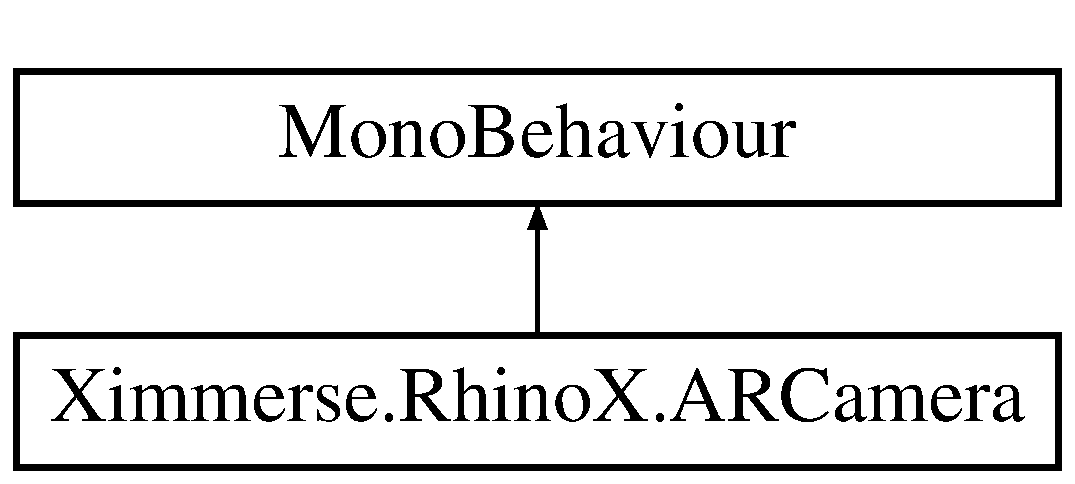
\includegraphics[height=2.000000cm]{class_ximmerse_1_1_rhino_x_1_1_a_r_camera}
\end{center}
\end{figure}
\subsection*{Public Member Functions}
\begin{DoxyCompactItemize}
\item 
bool \mbox{\hyperlink{class_ximmerse_1_1_rhino_x_1_1_a_r_camera_a4b8e8609b5b3c5cc7e9722be7e11caff}{Recenter\+Tracking}} (bool Yaw\+Only=true)
\begin{DoxyCompactList}\small\item\em Recenters the tracking. \end{DoxyCompactList}\item 
void \mbox{\hyperlink{class_ximmerse_1_1_rhino_x_1_1_a_r_camera_aefc6422a8587e8769e5e224c2ce66148}{Set\+Fov}} (float \mbox{\hyperlink{class_ximmerse_1_1_rhino_x_1_1_a_r_camera_ace7c430868896aa5cc911f023a0c4ec2}{h\+Fov}}, float \mbox{\hyperlink{class_ximmerse_1_1_rhino_x_1_1_a_r_camera_a386210a7a33ca8df7dd6fd8e0530bb55}{v\+Fov}})
\begin{DoxyCompactList}\small\item\em Sets the horizontal and vertical fov. \end{DoxyCompactList}\item 
void \mbox{\hyperlink{class_ximmerse_1_1_rhino_x_1_1_a_r_camera_a8990c22f1fd7eadc81fc8cce26e307ad}{Reset\+Fov}} ()
\begin{DoxyCompactList}\small\item\em Resets the horizontal and vertical fov. Default value \+: h\+Fov = 77.\+099 , h\+Fov = 77.\+099 \end{DoxyCompactList}\end{DoxyCompactItemize}
\subsection*{Static Public Member Functions}
\begin{DoxyCompactItemize}
\item 
\mbox{\Hypertarget{class_ximmerse_1_1_rhino_x_1_1_a_r_camera_a924a0d756c445884e15efabb10cd10bb}\label{class_ximmerse_1_1_rhino_x_1_1_a_r_camera_a924a0d756c445884e15efabb10cd10bb}} 
static Matrix4x4 {\bfseries Perspective} (float left, float right, float bottom, float top, float near, float far)
\end{DoxyCompactItemize}
\subsection*{Public Attributes}
\begin{DoxyCompactItemize}
\item 
\mbox{\Hypertarget{class_ximmerse_1_1_rhino_x_1_1_a_r_camera_a55c0080aa29097a34d1983755f32f73d}\label{class_ximmerse_1_1_rhino_x_1_1_a_r_camera_a55c0080aa29097a34d1983755f32f73d}} 
Vector3 {\bfseries m\+\_\+recenter\+CompP} = Vector3.\+zero
\item 
\mbox{\Hypertarget{class_ximmerse_1_1_rhino_x_1_1_a_r_camera_aa4a6340782612679e7010d0e28ad806d}\label{class_ximmerse_1_1_rhino_x_1_1_a_r_camera_aa4a6340782612679e7010d0e28ad806d}} 
Quaternion {\bfseries m\+\_\+recenter\+CompQ} = Quaternion.\+identity
\end{DoxyCompactItemize}
\subsection*{Static Public Attributes}
\begin{DoxyCompactItemize}
\item 
static float \mbox{\hyperlink{class_ximmerse_1_1_rhino_x_1_1_a_r_camera_ae47108706cc7216eaa7dd50ffbef8851}{k\+Light\+Center\+\_\+X}} = 0
\begin{DoxyCompactList}\small\item\em const projection matrix vertical offset (the m02 field of the projection matrix). This is the light center offset X \end{DoxyCompactList}\item 
static float \mbox{\hyperlink{class_ximmerse_1_1_rhino_x_1_1_a_r_camera_a78a8ef179a5c613db4aae90a15aa1ffd}{k\+Light\+Center\+\_\+Y}} = -\/0.\+0779f
\begin{DoxyCompactList}\small\item\em const projection matrix vertical offset (the m12 field of the projection matrix). This is the light center offset Y \end{DoxyCompactList}\end{DoxyCompactItemize}
\subsection*{Properties}
\begin{DoxyCompactItemize}
\item 
\mbox{\Hypertarget{class_ximmerse_1_1_rhino_x_1_1_a_r_camera_a2a7a6add621976cabf2958ea01f652fd}\label{class_ximmerse_1_1_rhino_x_1_1_a_r_camera_a2a7a6add621976cabf2958ea01f652fd}} 
static \mbox{\hyperlink{class_ximmerse_1_1_rhino_x_1_1_a_r_camera}{A\+R\+Camera}} {\bfseries Instance}\hspace{0.3cm}{\ttfamily  \mbox{[}get\mbox{]}}
\item 
float \mbox{\hyperlink{class_ximmerse_1_1_rhino_x_1_1_a_r_camera_a83ddafe725c4738c84b292501ea9e55f}{Inter\+Pupil\+Distance}}\hspace{0.3cm}{\ttfamily  \mbox{[}get, set\mbox{]}}
\begin{DoxyCompactList}\small\item\em I\+PD \+: inter pupil distance. Most common value is 0.\+062 (62mm), developer may customize this value . \end{DoxyCompactList}\item 
\mbox{\hyperlink{namespace_ximmerse_1_1_rhino_x_a6f6b7e0f3b580e31040b75578bbf4c94}{Anti\+Aliasing}} \mbox{\hyperlink{class_ximmerse_1_1_rhino_x_1_1_a_r_camera_ae64077302d7071482e8242b754af8af4}{Antialiasing}}\hspace{0.3cm}{\ttfamily  \mbox{[}get, set\mbox{]}}
\begin{DoxyCompactList}\small\item\em Gets or sets the anti aliasing level of eye image. \end{DoxyCompactList}\item 
bool \mbox{\hyperlink{class_ximmerse_1_1_rhino_x_1_1_a_r_camera_a6374e45b33643924d3aa0c3e32360d73}{Track\+Position}}\hspace{0.3cm}{\ttfamily  \mbox{[}get, set\mbox{]}}
\begin{DoxyCompactList}\small\item\em Should track position ? If set to use, position of head would not be updated by S\+DK. \end{DoxyCompactList}\item 
bool \mbox{\hyperlink{class_ximmerse_1_1_rhino_x_1_1_a_r_camera_ae2c6be1c7856874b2f66961adb1536ae}{Track\+Rotation}}\hspace{0.3cm}{\ttfamily  \mbox{[}get, set\mbox{]}}
\begin{DoxyCompactList}\small\item\em Should track rotation ? If set to use, rotation of head would not be updated by S\+DK. \end{DoxyCompactList}\item 
\mbox{\hyperlink{struct_ximmerse_1_1_rhino_x_1_1_pose}{Pose}} \mbox{\hyperlink{class_ximmerse_1_1_rhino_x_1_1_a_r_camera_afdc65a0a6965edba5243a12d34a4cb18}{Head\+Pose}}\hspace{0.3cm}{\ttfamily  \mbox{[}get\mbox{]}}
\begin{DoxyCompactList}\small\item\em Head pose (non predict) \end{DoxyCompactList}\item 
\mbox{\hyperlink{class_ximmerse_1_1_rhino_x_1_1_object_tracking_profile}{Object\+Tracking\+Profile}} \mbox{\hyperlink{class_ximmerse_1_1_rhino_x_1_1_a_r_camera_a3abfd51c012cf14af414f4c7df72de66}{Tracking\+Profile}}\hspace{0.3cm}{\ttfamily  \mbox{[}get, set\mbox{]}}
\begin{DoxyCompactList}\small\item\em Gets the currently loaded tag tracking profile. Sets this variable will cause the previous profile been unloaded, then the new one will be loaded. \end{DoxyCompactList}\item 
float \mbox{\hyperlink{class_ximmerse_1_1_rhino_x_1_1_a_r_camera_ace7c430868896aa5cc911f023a0c4ec2}{h\+Fov}}\hspace{0.3cm}{\ttfamily  \mbox{[}get\mbox{]}}
\begin{DoxyCompactList}\small\item\em Gets the horizontal field of view. By default this value = 77.\+091. \end{DoxyCompactList}\item 
float \mbox{\hyperlink{class_ximmerse_1_1_rhino_x_1_1_a_r_camera_a386210a7a33ca8df7dd6fd8e0530bb55}{v\+Fov}}\hspace{0.3cm}{\ttfamily  \mbox{[}get\mbox{]}}
\begin{DoxyCompactList}\small\item\em Gets the vertical field of view. By default this value = 77.\+091. \end{DoxyCompactList}\end{DoxyCompactItemize}
\subsection*{Events}
\begin{DoxyCompactItemize}
\item 
static System.\+Action$<$ Camera, Camera $>$ \mbox{\hyperlink{class_ximmerse_1_1_rhino_x_1_1_a_r_camera_a635b0074257b24358550492fa56389e7}{On\+Create\+Stereo\+Cameras}} = null
\begin{DoxyCompactList}\small\item\em Event is fired after stereo eyes are created. Developers can add post effect scripts on this event. First camera parameter = left eye camera; Second camera parameter = right eye camera; \end{DoxyCompactList}\end{DoxyCompactItemize}


\subsection{Detailed Description}
AR camera is the script that represents virtual camera in AR world. Developer may get the position/rotation of current head transform. 

AR camera \+: rendering 

\subsection{Member Function Documentation}
\mbox{\Hypertarget{class_ximmerse_1_1_rhino_x_1_1_a_r_camera_a4b8e8609b5b3c5cc7e9722be7e11caff}\label{class_ximmerse_1_1_rhino_x_1_1_a_r_camera_a4b8e8609b5b3c5cc7e9722be7e11caff}} 
\index{Ximmerse\+::\+Rhino\+X\+::\+A\+R\+Camera@{Ximmerse\+::\+Rhino\+X\+::\+A\+R\+Camera}!Recenter\+Tracking@{Recenter\+Tracking}}
\index{Recenter\+Tracking@{Recenter\+Tracking}!Ximmerse\+::\+Rhino\+X\+::\+A\+R\+Camera@{Ximmerse\+::\+Rhino\+X\+::\+A\+R\+Camera}}
\subsubsection{\texorpdfstring{Recenter\+Tracking()}{RecenterTracking()}}
{\footnotesize\ttfamily bool Ximmerse.\+Rhino\+X.\+A\+R\+Camera.\+Recenter\+Tracking (\begin{DoxyParamCaption}\item[{bool}]{Yaw\+Only = {\ttfamily true} }\end{DoxyParamCaption})\hspace{0.3cm}{\ttfamily [inline]}}



Recenters the tracking. 

\begin{DoxyReturn}{Returns}
{\ttfamily true}, if tracking was recentered, {\ttfamily false} otherwise.
\end{DoxyReturn}
\mbox{\Hypertarget{class_ximmerse_1_1_rhino_x_1_1_a_r_camera_a8990c22f1fd7eadc81fc8cce26e307ad}\label{class_ximmerse_1_1_rhino_x_1_1_a_r_camera_a8990c22f1fd7eadc81fc8cce26e307ad}} 
\index{Ximmerse\+::\+Rhino\+X\+::\+A\+R\+Camera@{Ximmerse\+::\+Rhino\+X\+::\+A\+R\+Camera}!Reset\+Fov@{Reset\+Fov}}
\index{Reset\+Fov@{Reset\+Fov}!Ximmerse\+::\+Rhino\+X\+::\+A\+R\+Camera@{Ximmerse\+::\+Rhino\+X\+::\+A\+R\+Camera}}
\subsubsection{\texorpdfstring{Reset\+Fov()}{ResetFov()}}
{\footnotesize\ttfamily void Ximmerse.\+Rhino\+X.\+A\+R\+Camera.\+Reset\+Fov (\begin{DoxyParamCaption}{ }\end{DoxyParamCaption})\hspace{0.3cm}{\ttfamily [inline]}}



Resets the horizontal and vertical fov. Default value \+: h\+Fov = 77.\+099 , h\+Fov = 77.\+099 

\mbox{\Hypertarget{class_ximmerse_1_1_rhino_x_1_1_a_r_camera_aefc6422a8587e8769e5e224c2ce66148}\label{class_ximmerse_1_1_rhino_x_1_1_a_r_camera_aefc6422a8587e8769e5e224c2ce66148}} 
\index{Ximmerse\+::\+Rhino\+X\+::\+A\+R\+Camera@{Ximmerse\+::\+Rhino\+X\+::\+A\+R\+Camera}!Set\+Fov@{Set\+Fov}}
\index{Set\+Fov@{Set\+Fov}!Ximmerse\+::\+Rhino\+X\+::\+A\+R\+Camera@{Ximmerse\+::\+Rhino\+X\+::\+A\+R\+Camera}}
\subsubsection{\texorpdfstring{Set\+Fov()}{SetFov()}}
{\footnotesize\ttfamily void Ximmerse.\+Rhino\+X.\+A\+R\+Camera.\+Set\+Fov (\begin{DoxyParamCaption}\item[{float}]{h\+Fov,  }\item[{float}]{v\+Fov }\end{DoxyParamCaption})\hspace{0.3cm}{\ttfamily [inline]}}



Sets the horizontal and vertical fov. 

\begin{DoxyReturn}{Returns}
The fov.
\end{DoxyReturn}

\begin{DoxyParams}{Parameters}
{\em h\+Fov} & H fov.\\
\hline
{\em v\+Fov} & V fov.\\
\hline
\end{DoxyParams}


\subsection{Member Data Documentation}
\mbox{\Hypertarget{class_ximmerse_1_1_rhino_x_1_1_a_r_camera_ae47108706cc7216eaa7dd50ffbef8851}\label{class_ximmerse_1_1_rhino_x_1_1_a_r_camera_ae47108706cc7216eaa7dd50ffbef8851}} 
\index{Ximmerse\+::\+Rhino\+X\+::\+A\+R\+Camera@{Ximmerse\+::\+Rhino\+X\+::\+A\+R\+Camera}!k\+Light\+Center\+\_\+X@{k\+Light\+Center\+\_\+X}}
\index{k\+Light\+Center\+\_\+X@{k\+Light\+Center\+\_\+X}!Ximmerse\+::\+Rhino\+X\+::\+A\+R\+Camera@{Ximmerse\+::\+Rhino\+X\+::\+A\+R\+Camera}}
\subsubsection{\texorpdfstring{k\+Light\+Center\+\_\+X}{kLightCenter\_X}}
{\footnotesize\ttfamily float Ximmerse.\+Rhino\+X.\+A\+R\+Camera.\+k\+Light\+Center\+\_\+X = 0\hspace{0.3cm}{\ttfamily [static]}}



const projection matrix vertical offset (the m02 field of the projection matrix). This is the light center offset X 

\mbox{\Hypertarget{class_ximmerse_1_1_rhino_x_1_1_a_r_camera_a78a8ef179a5c613db4aae90a15aa1ffd}\label{class_ximmerse_1_1_rhino_x_1_1_a_r_camera_a78a8ef179a5c613db4aae90a15aa1ffd}} 
\index{Ximmerse\+::\+Rhino\+X\+::\+A\+R\+Camera@{Ximmerse\+::\+Rhino\+X\+::\+A\+R\+Camera}!k\+Light\+Center\+\_\+Y@{k\+Light\+Center\+\_\+Y}}
\index{k\+Light\+Center\+\_\+Y@{k\+Light\+Center\+\_\+Y}!Ximmerse\+::\+Rhino\+X\+::\+A\+R\+Camera@{Ximmerse\+::\+Rhino\+X\+::\+A\+R\+Camera}}
\subsubsection{\texorpdfstring{k\+Light\+Center\+\_\+Y}{kLightCenter\_Y}}
{\footnotesize\ttfamily float Ximmerse.\+Rhino\+X.\+A\+R\+Camera.\+k\+Light\+Center\+\_\+Y = -\/0.\+0779f\hspace{0.3cm}{\ttfamily [static]}}



const projection matrix vertical offset (the m12 field of the projection matrix). This is the light center offset Y 



\subsection{Property Documentation}
\mbox{\Hypertarget{class_ximmerse_1_1_rhino_x_1_1_a_r_camera_ae64077302d7071482e8242b754af8af4}\label{class_ximmerse_1_1_rhino_x_1_1_a_r_camera_ae64077302d7071482e8242b754af8af4}} 
\index{Ximmerse\+::\+Rhino\+X\+::\+A\+R\+Camera@{Ximmerse\+::\+Rhino\+X\+::\+A\+R\+Camera}!Antialiasing@{Antialiasing}}
\index{Antialiasing@{Antialiasing}!Ximmerse\+::\+Rhino\+X\+::\+A\+R\+Camera@{Ximmerse\+::\+Rhino\+X\+::\+A\+R\+Camera}}
\subsubsection{\texorpdfstring{Antialiasing}{Antialiasing}}
{\footnotesize\ttfamily \mbox{\hyperlink{namespace_ximmerse_1_1_rhino_x_a6f6b7e0f3b580e31040b75578bbf4c94}{Anti\+Aliasing}} Ximmerse.\+Rhino\+X.\+A\+R\+Camera.\+Antialiasing\hspace{0.3cm}{\ttfamily [get]}, {\ttfamily [set]}}



Gets or sets the anti aliasing level of eye image. 

The anti aliasing.\mbox{\Hypertarget{class_ximmerse_1_1_rhino_x_1_1_a_r_camera_afdc65a0a6965edba5243a12d34a4cb18}\label{class_ximmerse_1_1_rhino_x_1_1_a_r_camera_afdc65a0a6965edba5243a12d34a4cb18}} 
\index{Ximmerse\+::\+Rhino\+X\+::\+A\+R\+Camera@{Ximmerse\+::\+Rhino\+X\+::\+A\+R\+Camera}!Head\+Pose@{Head\+Pose}}
\index{Head\+Pose@{Head\+Pose}!Ximmerse\+::\+Rhino\+X\+::\+A\+R\+Camera@{Ximmerse\+::\+Rhino\+X\+::\+A\+R\+Camera}}
\subsubsection{\texorpdfstring{Head\+Pose}{HeadPose}}
{\footnotesize\ttfamily \mbox{\hyperlink{struct_ximmerse_1_1_rhino_x_1_1_pose}{Pose}} Ximmerse.\+Rhino\+X.\+A\+R\+Camera.\+Head\+Pose\hspace{0.3cm}{\ttfamily [get]}}



Head pose (non predict) 

Gets the current V\+IO output head pose. 

The predict head pose.\mbox{\Hypertarget{class_ximmerse_1_1_rhino_x_1_1_a_r_camera_ace7c430868896aa5cc911f023a0c4ec2}\label{class_ximmerse_1_1_rhino_x_1_1_a_r_camera_ace7c430868896aa5cc911f023a0c4ec2}} 
\index{Ximmerse\+::\+Rhino\+X\+::\+A\+R\+Camera@{Ximmerse\+::\+Rhino\+X\+::\+A\+R\+Camera}!h\+Fov@{h\+Fov}}
\index{h\+Fov@{h\+Fov}!Ximmerse\+::\+Rhino\+X\+::\+A\+R\+Camera@{Ximmerse\+::\+Rhino\+X\+::\+A\+R\+Camera}}
\subsubsection{\texorpdfstring{h\+Fov}{hFov}}
{\footnotesize\ttfamily float Ximmerse.\+Rhino\+X.\+A\+R\+Camera.\+h\+Fov\hspace{0.3cm}{\ttfamily [get]}}



Gets the horizontal field of view. By default this value = 77.\+091. 

The h fov.\mbox{\Hypertarget{class_ximmerse_1_1_rhino_x_1_1_a_r_camera_a83ddafe725c4738c84b292501ea9e55f}\label{class_ximmerse_1_1_rhino_x_1_1_a_r_camera_a83ddafe725c4738c84b292501ea9e55f}} 
\index{Ximmerse\+::\+Rhino\+X\+::\+A\+R\+Camera@{Ximmerse\+::\+Rhino\+X\+::\+A\+R\+Camera}!Inter\+Pupil\+Distance@{Inter\+Pupil\+Distance}}
\index{Inter\+Pupil\+Distance@{Inter\+Pupil\+Distance}!Ximmerse\+::\+Rhino\+X\+::\+A\+R\+Camera@{Ximmerse\+::\+Rhino\+X\+::\+A\+R\+Camera}}
\subsubsection{\texorpdfstring{Inter\+Pupil\+Distance}{InterPupilDistance}}
{\footnotesize\ttfamily float Ximmerse.\+Rhino\+X.\+A\+R\+Camera.\+Inter\+Pupil\+Distance\hspace{0.3cm}{\ttfamily [get]}, {\ttfamily [set]}}



I\+PD \+: inter pupil distance. Most common value is 0.\+062 (62mm), developer may customize this value . 

The inter pupil distance.\mbox{\Hypertarget{class_ximmerse_1_1_rhino_x_1_1_a_r_camera_a3abfd51c012cf14af414f4c7df72de66}\label{class_ximmerse_1_1_rhino_x_1_1_a_r_camera_a3abfd51c012cf14af414f4c7df72de66}} 
\index{Ximmerse\+::\+Rhino\+X\+::\+A\+R\+Camera@{Ximmerse\+::\+Rhino\+X\+::\+A\+R\+Camera}!Tracking\+Profile@{Tracking\+Profile}}
\index{Tracking\+Profile@{Tracking\+Profile}!Ximmerse\+::\+Rhino\+X\+::\+A\+R\+Camera@{Ximmerse\+::\+Rhino\+X\+::\+A\+R\+Camera}}
\subsubsection{\texorpdfstring{Tracking\+Profile}{TrackingProfile}}
{\footnotesize\ttfamily \mbox{\hyperlink{class_ximmerse_1_1_rhino_x_1_1_object_tracking_profile}{Object\+Tracking\+Profile}} Ximmerse.\+Rhino\+X.\+A\+R\+Camera.\+Tracking\+Profile\hspace{0.3cm}{\ttfamily [get]}, {\ttfamily [set]}}



Gets the currently loaded tag tracking profile. Sets this variable will cause the previous profile been unloaded, then the new one will be loaded. 

The tracking profile.\mbox{\Hypertarget{class_ximmerse_1_1_rhino_x_1_1_a_r_camera_a6374e45b33643924d3aa0c3e32360d73}\label{class_ximmerse_1_1_rhino_x_1_1_a_r_camera_a6374e45b33643924d3aa0c3e32360d73}} 
\index{Ximmerse\+::\+Rhino\+X\+::\+A\+R\+Camera@{Ximmerse\+::\+Rhino\+X\+::\+A\+R\+Camera}!Track\+Position@{Track\+Position}}
\index{Track\+Position@{Track\+Position}!Ximmerse\+::\+Rhino\+X\+::\+A\+R\+Camera@{Ximmerse\+::\+Rhino\+X\+::\+A\+R\+Camera}}
\subsubsection{\texorpdfstring{Track\+Position}{TrackPosition}}
{\footnotesize\ttfamily bool Ximmerse.\+Rhino\+X.\+A\+R\+Camera.\+Track\+Position\hspace{0.3cm}{\ttfamily [get]}, {\ttfamily [set]}}



Should track position ? If set to use, position of head would not be updated by S\+DK. 

{\ttfamily true} if shoud track position; otherwise, {\ttfamily false}.\mbox{\Hypertarget{class_ximmerse_1_1_rhino_x_1_1_a_r_camera_ae2c6be1c7856874b2f66961adb1536ae}\label{class_ximmerse_1_1_rhino_x_1_1_a_r_camera_ae2c6be1c7856874b2f66961adb1536ae}} 
\index{Ximmerse\+::\+Rhino\+X\+::\+A\+R\+Camera@{Ximmerse\+::\+Rhino\+X\+::\+A\+R\+Camera}!Track\+Rotation@{Track\+Rotation}}
\index{Track\+Rotation@{Track\+Rotation}!Ximmerse\+::\+Rhino\+X\+::\+A\+R\+Camera@{Ximmerse\+::\+Rhino\+X\+::\+A\+R\+Camera}}
\subsubsection{\texorpdfstring{Track\+Rotation}{TrackRotation}}
{\footnotesize\ttfamily bool Ximmerse.\+Rhino\+X.\+A\+R\+Camera.\+Track\+Rotation\hspace{0.3cm}{\ttfamily [get]}, {\ttfamily [set]}}



Should track rotation ? If set to use, rotation of head would not be updated by S\+DK. 

{\ttfamily true} if shoud track position; otherwise, {\ttfamily false}.\mbox{\Hypertarget{class_ximmerse_1_1_rhino_x_1_1_a_r_camera_a386210a7a33ca8df7dd6fd8e0530bb55}\label{class_ximmerse_1_1_rhino_x_1_1_a_r_camera_a386210a7a33ca8df7dd6fd8e0530bb55}} 
\index{Ximmerse\+::\+Rhino\+X\+::\+A\+R\+Camera@{Ximmerse\+::\+Rhino\+X\+::\+A\+R\+Camera}!v\+Fov@{v\+Fov}}
\index{v\+Fov@{v\+Fov}!Ximmerse\+::\+Rhino\+X\+::\+A\+R\+Camera@{Ximmerse\+::\+Rhino\+X\+::\+A\+R\+Camera}}
\subsubsection{\texorpdfstring{v\+Fov}{vFov}}
{\footnotesize\ttfamily float Ximmerse.\+Rhino\+X.\+A\+R\+Camera.\+v\+Fov\hspace{0.3cm}{\ttfamily [get]}}



Gets the vertical field of view. By default this value = 77.\+091. 

The v fov.

\subsection{Event Documentation}
\mbox{\Hypertarget{class_ximmerse_1_1_rhino_x_1_1_a_r_camera_a635b0074257b24358550492fa56389e7}\label{class_ximmerse_1_1_rhino_x_1_1_a_r_camera_a635b0074257b24358550492fa56389e7}} 
\index{Ximmerse\+::\+Rhino\+X\+::\+A\+R\+Camera@{Ximmerse\+::\+Rhino\+X\+::\+A\+R\+Camera}!On\+Create\+Stereo\+Cameras@{On\+Create\+Stereo\+Cameras}}
\index{On\+Create\+Stereo\+Cameras@{On\+Create\+Stereo\+Cameras}!Ximmerse\+::\+Rhino\+X\+::\+A\+R\+Camera@{Ximmerse\+::\+Rhino\+X\+::\+A\+R\+Camera}}
\subsubsection{\texorpdfstring{On\+Create\+Stereo\+Cameras}{OnCreateStereoCameras}}
{\footnotesize\ttfamily System.\+Action$<$Camera, Camera$>$ Ximmerse.\+Rhino\+X.\+A\+R\+Camera.\+On\+Create\+Stereo\+Cameras = null\hspace{0.3cm}{\ttfamily [static]}}



Event is fired after stereo eyes are created. Developers can add post effect scripts on this event. First camera parameter = left eye camera; Second camera parameter = right eye camera; 



The documentation for this class was generated from the following files\+:\begin{DoxyCompactItemize}
\item 
A\+R\+Camera.\+cs\item 
A\+R\+Camera\+\_\+\+Rendering.\+cs\end{DoxyCompactItemize}

\hypertarget{class_ximmerse_1_1_rhino_x_1_1_calibration_serialization_data}{}\section{Ximmerse.\+Rhino\+X.\+Calibration\+Serialization\+Data Class Reference}
\label{class_ximmerse_1_1_rhino_x_1_1_calibration_serialization_data}\index{Ximmerse.\+Rhino\+X.\+Calibration\+Serialization\+Data@{Ximmerse.\+Rhino\+X.\+Calibration\+Serialization\+Data}}


Calibration serialization data. 用于持久化的数据格式。  


\subsection*{Public Member Functions}
\begin{DoxyCompactItemize}
\item 
\mbox{\Hypertarget{class_ximmerse_1_1_rhino_x_1_1_calibration_serialization_data_acf57cae12382f29c523b48463346eba3}\label{class_ximmerse_1_1_rhino_x_1_1_calibration_serialization_data_acf57cae12382f29c523b48463346eba3}} 
byte \mbox{[}$\,$\mbox{]} {\bfseries Serialize\+To\+Bytes} ()
\end{DoxyCompactItemize}
\subsection*{Static Public Member Functions}
\begin{DoxyCompactItemize}
\item 
static \mbox{\hyperlink{class_ximmerse_1_1_rhino_x_1_1_calibration_serialization_data}{Calibration\+Serialization\+Data}} \mbox{\hyperlink{class_ximmerse_1_1_rhino_x_1_1_calibration_serialization_data_ab86d9a60c838e8fe8503f0b9126ef86e}{Deserialize}} (byte\mbox{[}$\,$\mbox{]} buffers, ref int pointer)
\begin{DoxyCompactList}\small\item\em Deserialize the specified buffers in pointer. \end{DoxyCompactList}\item 
\mbox{\Hypertarget{class_ximmerse_1_1_rhino_x_1_1_calibration_serialization_data_abc749af23b37e44fa30a78afe8272f9e}\label{class_ximmerse_1_1_rhino_x_1_1_calibration_serialization_data_abc749af23b37e44fa30a78afe8272f9e}} 
static List$<$ \mbox{\hyperlink{class_ximmerse_1_1_rhino_x_1_1_calibration_serialization_data}{Calibration\+Serialization\+Data}} $>$ {\bfseries Deserialize\+To\+List} (byte\mbox{[}$\,$\mbox{]} buffer)
\end{DoxyCompactItemize}
\subsection*{Public Attributes}
\begin{DoxyCompactItemize}
\item 
int \mbox{\hyperlink{class_ximmerse_1_1_rhino_x_1_1_calibration_serialization_data_a40dcec53e2ae1967cf4ef5aedff63c92}{Self\+ID}}
\begin{DoxyCompactList}\small\item\em The marker ID represents \char`\"{}self\char`\"{} \end{DoxyCompactList}\item 
int \mbox{\hyperlink{class_ximmerse_1_1_rhino_x_1_1_calibration_serialization_data_acc2ded62f0e4db7e4284f11494babd5b}{Other\+ID}}
\begin{DoxyCompactList}\small\item\em The marker ID represents \char`\"{}other\char`\"{} \end{DoxyCompactList}\item 
Vector3 \mbox{\hyperlink{class_ximmerse_1_1_rhino_x_1_1_calibration_serialization_data_a8919018eed725bf6c85ed9b1b32d4bdf}{P\+\_\+\+Self2\+Other}}
\begin{DoxyCompactList}\small\item\em Position transfer self to other space \end{DoxyCompactList}\item 
Quaternion \mbox{\hyperlink{class_ximmerse_1_1_rhino_x_1_1_calibration_serialization_data_addd1ca5772b4c8fb9408383c5b7f6d99}{Q\+\_\+\+Self2\+Other}}
\begin{DoxyCompactList}\small\item\em Rotation transfer self to other space \end{DoxyCompactList}\item 
Vector3 \mbox{\hyperlink{class_ximmerse_1_1_rhino_x_1_1_calibration_serialization_data_a7d0239f8ee5618360d38e600ed4a4b2e}{P\+\_\+\+Other2\+Self}}
\begin{DoxyCompactList}\small\item\em Position transfer other to self space \end{DoxyCompactList}\item 
Quaternion \mbox{\hyperlink{class_ximmerse_1_1_rhino_x_1_1_calibration_serialization_data_a3988b74a9fe9394d03197c6e386ccfb6}{Q\+\_\+\+Other2\+Self}}
\begin{DoxyCompactList}\small\item\em Rotation transfer other to self space \end{DoxyCompactList}\end{DoxyCompactItemize}
\subsection*{Properties}
\begin{DoxyCompactItemize}
\item 
\mbox{\Hypertarget{class_ximmerse_1_1_rhino_x_1_1_calibration_serialization_data_a1485e91da74bc2ad82ba0e3d4aeb6df3}\label{class_ximmerse_1_1_rhino_x_1_1_calibration_serialization_data_a1485e91da74bc2ad82ba0e3d4aeb6df3}} 
static int {\bfseries Size}\hspace{0.3cm}{\ttfamily  \mbox{[}get\mbox{]}}
\end{DoxyCompactItemize}


\subsection{Detailed Description}
Calibration serialization data. 用于持久化的数据格式。 



\subsection{Member Function Documentation}
\mbox{\Hypertarget{class_ximmerse_1_1_rhino_x_1_1_calibration_serialization_data_ab86d9a60c838e8fe8503f0b9126ef86e}\label{class_ximmerse_1_1_rhino_x_1_1_calibration_serialization_data_ab86d9a60c838e8fe8503f0b9126ef86e}} 
\index{Ximmerse\+::\+Rhino\+X\+::\+Calibration\+Serialization\+Data@{Ximmerse\+::\+Rhino\+X\+::\+Calibration\+Serialization\+Data}!Deserialize@{Deserialize}}
\index{Deserialize@{Deserialize}!Ximmerse\+::\+Rhino\+X\+::\+Calibration\+Serialization\+Data@{Ximmerse\+::\+Rhino\+X\+::\+Calibration\+Serialization\+Data}}
\subsubsection{\texorpdfstring{Deserialize()}{Deserialize()}}
{\footnotesize\ttfamily static \mbox{\hyperlink{class_ximmerse_1_1_rhino_x_1_1_calibration_serialization_data}{Calibration\+Serialization\+Data}} Ximmerse.\+Rhino\+X.\+Calibration\+Serialization\+Data.\+Deserialize (\begin{DoxyParamCaption}\item[{byte \mbox{[}$\,$\mbox{]}}]{buffers,  }\item[{ref int}]{pointer }\end{DoxyParamCaption})\hspace{0.3cm}{\ttfamily [inline]}, {\ttfamily [static]}}



Deserialize the specified buffers in pointer. 

\begin{DoxyReturn}{Returns}
The deserialize.
\end{DoxyReturn}

\begin{DoxyParams}{Parameters}
{\em buffers} & Buffers.\\
\hline
{\em pointer} & Pointer.\\
\hline
\end{DoxyParams}


\subsection{Member Data Documentation}
\mbox{\Hypertarget{class_ximmerse_1_1_rhino_x_1_1_calibration_serialization_data_acc2ded62f0e4db7e4284f11494babd5b}\label{class_ximmerse_1_1_rhino_x_1_1_calibration_serialization_data_acc2ded62f0e4db7e4284f11494babd5b}} 
\index{Ximmerse\+::\+Rhino\+X\+::\+Calibration\+Serialization\+Data@{Ximmerse\+::\+Rhino\+X\+::\+Calibration\+Serialization\+Data}!Other\+ID@{Other\+ID}}
\index{Other\+ID@{Other\+ID}!Ximmerse\+::\+Rhino\+X\+::\+Calibration\+Serialization\+Data@{Ximmerse\+::\+Rhino\+X\+::\+Calibration\+Serialization\+Data}}
\subsubsection{\texorpdfstring{Other\+ID}{OtherID}}
{\footnotesize\ttfamily int Ximmerse.\+Rhino\+X.\+Calibration\+Serialization\+Data.\+Other\+ID}



The marker ID represents \char`\"{}other\char`\"{} 

\mbox{\Hypertarget{class_ximmerse_1_1_rhino_x_1_1_calibration_serialization_data_a7d0239f8ee5618360d38e600ed4a4b2e}\label{class_ximmerse_1_1_rhino_x_1_1_calibration_serialization_data_a7d0239f8ee5618360d38e600ed4a4b2e}} 
\index{Ximmerse\+::\+Rhino\+X\+::\+Calibration\+Serialization\+Data@{Ximmerse\+::\+Rhino\+X\+::\+Calibration\+Serialization\+Data}!P\+\_\+\+Other2\+Self@{P\+\_\+\+Other2\+Self}}
\index{P\+\_\+\+Other2\+Self@{P\+\_\+\+Other2\+Self}!Ximmerse\+::\+Rhino\+X\+::\+Calibration\+Serialization\+Data@{Ximmerse\+::\+Rhino\+X\+::\+Calibration\+Serialization\+Data}}
\subsubsection{\texorpdfstring{P\+\_\+\+Other2\+Self}{P\_Other2Self}}
{\footnotesize\ttfamily Vector3 Ximmerse.\+Rhino\+X.\+Calibration\+Serialization\+Data.\+P\+\_\+\+Other2\+Self}



Position transfer other to self space 

\mbox{\Hypertarget{class_ximmerse_1_1_rhino_x_1_1_calibration_serialization_data_a8919018eed725bf6c85ed9b1b32d4bdf}\label{class_ximmerse_1_1_rhino_x_1_1_calibration_serialization_data_a8919018eed725bf6c85ed9b1b32d4bdf}} 
\index{Ximmerse\+::\+Rhino\+X\+::\+Calibration\+Serialization\+Data@{Ximmerse\+::\+Rhino\+X\+::\+Calibration\+Serialization\+Data}!P\+\_\+\+Self2\+Other@{P\+\_\+\+Self2\+Other}}
\index{P\+\_\+\+Self2\+Other@{P\+\_\+\+Self2\+Other}!Ximmerse\+::\+Rhino\+X\+::\+Calibration\+Serialization\+Data@{Ximmerse\+::\+Rhino\+X\+::\+Calibration\+Serialization\+Data}}
\subsubsection{\texorpdfstring{P\+\_\+\+Self2\+Other}{P\_Self2Other}}
{\footnotesize\ttfamily Vector3 Ximmerse.\+Rhino\+X.\+Calibration\+Serialization\+Data.\+P\+\_\+\+Self2\+Other}



Position transfer self to other space 

\mbox{\Hypertarget{class_ximmerse_1_1_rhino_x_1_1_calibration_serialization_data_a3988b74a9fe9394d03197c6e386ccfb6}\label{class_ximmerse_1_1_rhino_x_1_1_calibration_serialization_data_a3988b74a9fe9394d03197c6e386ccfb6}} 
\index{Ximmerse\+::\+Rhino\+X\+::\+Calibration\+Serialization\+Data@{Ximmerse\+::\+Rhino\+X\+::\+Calibration\+Serialization\+Data}!Q\+\_\+\+Other2\+Self@{Q\+\_\+\+Other2\+Self}}
\index{Q\+\_\+\+Other2\+Self@{Q\+\_\+\+Other2\+Self}!Ximmerse\+::\+Rhino\+X\+::\+Calibration\+Serialization\+Data@{Ximmerse\+::\+Rhino\+X\+::\+Calibration\+Serialization\+Data}}
\subsubsection{\texorpdfstring{Q\+\_\+\+Other2\+Self}{Q\_Other2Self}}
{\footnotesize\ttfamily Quaternion Ximmerse.\+Rhino\+X.\+Calibration\+Serialization\+Data.\+Q\+\_\+\+Other2\+Self}



Rotation transfer other to self space 

\mbox{\Hypertarget{class_ximmerse_1_1_rhino_x_1_1_calibration_serialization_data_addd1ca5772b4c8fb9408383c5b7f6d99}\label{class_ximmerse_1_1_rhino_x_1_1_calibration_serialization_data_addd1ca5772b4c8fb9408383c5b7f6d99}} 
\index{Ximmerse\+::\+Rhino\+X\+::\+Calibration\+Serialization\+Data@{Ximmerse\+::\+Rhino\+X\+::\+Calibration\+Serialization\+Data}!Q\+\_\+\+Self2\+Other@{Q\+\_\+\+Self2\+Other}}
\index{Q\+\_\+\+Self2\+Other@{Q\+\_\+\+Self2\+Other}!Ximmerse\+::\+Rhino\+X\+::\+Calibration\+Serialization\+Data@{Ximmerse\+::\+Rhino\+X\+::\+Calibration\+Serialization\+Data}}
\subsubsection{\texorpdfstring{Q\+\_\+\+Self2\+Other}{Q\_Self2Other}}
{\footnotesize\ttfamily Quaternion Ximmerse.\+Rhino\+X.\+Calibration\+Serialization\+Data.\+Q\+\_\+\+Self2\+Other}



Rotation transfer self to other space 

\mbox{\Hypertarget{class_ximmerse_1_1_rhino_x_1_1_calibration_serialization_data_a40dcec53e2ae1967cf4ef5aedff63c92}\label{class_ximmerse_1_1_rhino_x_1_1_calibration_serialization_data_a40dcec53e2ae1967cf4ef5aedff63c92}} 
\index{Ximmerse\+::\+Rhino\+X\+::\+Calibration\+Serialization\+Data@{Ximmerse\+::\+Rhino\+X\+::\+Calibration\+Serialization\+Data}!Self\+ID@{Self\+ID}}
\index{Self\+ID@{Self\+ID}!Ximmerse\+::\+Rhino\+X\+::\+Calibration\+Serialization\+Data@{Ximmerse\+::\+Rhino\+X\+::\+Calibration\+Serialization\+Data}}
\subsubsection{\texorpdfstring{Self\+ID}{SelfID}}
{\footnotesize\ttfamily int Ximmerse.\+Rhino\+X.\+Calibration\+Serialization\+Data.\+Self\+ID}



The marker ID represents \char`\"{}self\char`\"{} 



The documentation for this class was generated from the following file\+:\begin{DoxyCompactItemize}
\item 
Calibration/Calibration\+Serialization\+Data.\+cs\end{DoxyCompactItemize}

\hypertarget{class_ximmerse_1_1_rhino_x_1_1_tracked_object_json_1_1_card_group_json}{}\section{Ximmerse.\+Rhino\+X.\+Tracked\+Object\+Json.\+Card\+Group\+Json Class Reference}
\label{class_ximmerse_1_1_rhino_x_1_1_tracked_object_json_1_1_card_group_json}\index{Ximmerse.\+Rhino\+X.\+Tracked\+Object\+Json.\+Card\+Group\+Json@{Ximmerse.\+Rhino\+X.\+Tracked\+Object\+Json.\+Card\+Group\+Json}}
\subsection*{Public Attributes}
\begin{DoxyCompactItemize}
\item 
\mbox{\Hypertarget{class_ximmerse_1_1_rhino_x_1_1_tracked_object_json_1_1_card_group_json_a5f31de6baa714b3f23c858ddf627afe1}\label{class_ximmerse_1_1_rhino_x_1_1_tracked_object_json_1_1_card_group_json_a5f31de6baa714b3f23c858ddf627afe1}} 
string {\bfseries Calib\+File}
\item 
\mbox{\Hypertarget{class_ximmerse_1_1_rhino_x_1_1_tracked_object_json_1_1_card_group_json_ab6f414b2d3dec5cbb3cd9d6074bb9499}\label{class_ximmerse_1_1_rhino_x_1_1_tracked_object_json_1_1_card_group_json_ab6f414b2d3dec5cbb3cd9d6074bb9499}} 
string {\bfseries Mode\+Type}
\item 
\mbox{\Hypertarget{class_ximmerse_1_1_rhino_x_1_1_tracked_object_json_1_1_card_group_json_a6e53696fe2fb2794768f581234e3246c}\label{class_ximmerse_1_1_rhino_x_1_1_tracked_object_json_1_1_card_group_json_a6e53696fe2fb2794768f581234e3246c}} 
int {\bfseries Group\+ID}
\item 
\mbox{\Hypertarget{class_ximmerse_1_1_rhino_x_1_1_tracked_object_json_1_1_card_group_json_aab995bd10c5775dacb54eadb0a1601e7}\label{class_ximmerse_1_1_rhino_x_1_1_tracked_object_json_1_1_card_group_json_aab995bd10c5775dacb54eadb0a1601e7}} 
int \mbox{[}$\,$\mbox{]} {\bfseries Markers}
\item 
\mbox{\Hypertarget{class_ximmerse_1_1_rhino_x_1_1_tracked_object_json_1_1_card_group_json_a917db29e1342780c1993a18d4184f143}\label{class_ximmerse_1_1_rhino_x_1_1_tracked_object_json_1_1_card_group_json_a917db29e1342780c1993a18d4184f143}} 
float \mbox{[}$\,$\mbox{]} {\bfseries Markers\+Size}
\end{DoxyCompactItemize}


The documentation for this class was generated from the following file\+:\begin{DoxyCompactItemize}
\item 
Tracked\+Object\+Json.\+cs\end{DoxyCompactItemize}

\hypertarget{class_ximmerse_1_1_rhino_x_1_1_composite_ground_plane}{}\section{Ximmerse.\+Rhino\+X.\+Composite\+Ground\+Plane Class Reference}
\label{class_ximmerse_1_1_rhino_x_1_1_composite_ground_plane}\index{Ximmerse.\+Rhino\+X.\+Composite\+Ground\+Plane@{Ximmerse.\+Rhino\+X.\+Composite\+Ground\+Plane}}


Composite ground plane \+: composite of multiple ground plane to align the head pose. Composite ground plane should be singleton in your scene.  


Inheritance diagram for Ximmerse.\+Rhino\+X.\+Composite\+Ground\+Plane\+:\begin{figure}[H]
\begin{center}
\leavevmode
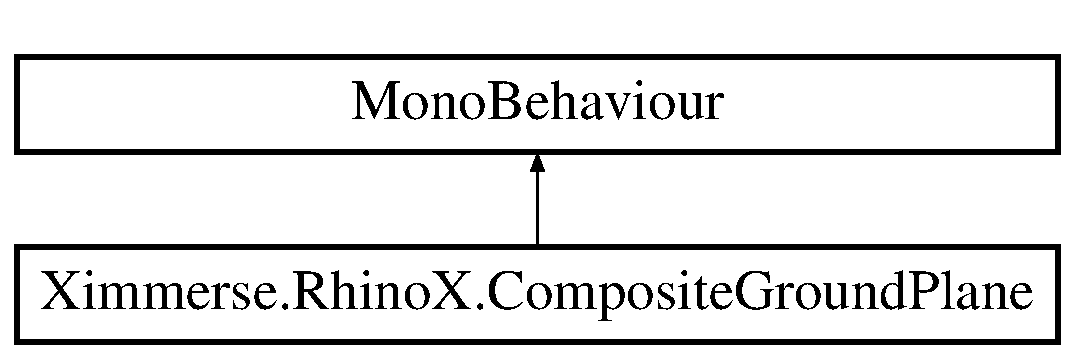
\includegraphics[height=2.000000cm]{class_ximmerse_1_1_rhino_x_1_1_composite_ground_plane}
\end{center}
\end{figure}
\subsection*{Public Types}
\begin{DoxyCompactItemize}
\item 
enum \mbox{\hyperlink{class_ximmerse_1_1_rhino_x_1_1_composite_ground_plane_a04f66929fadbcaaf0d0f9c53cd856dfd}{Recenter\+Mode}} \{ \mbox{\hyperlink{class_ximmerse_1_1_rhino_x_1_1_composite_ground_plane_a04f66929fadbcaaf0d0f9c53cd856dfdae7052705ca5b1918757966609990e511}{Recenter\+Mode.\+Everyframe}} = 0, 
\mbox{\hyperlink{class_ximmerse_1_1_rhino_x_1_1_composite_ground_plane_a04f66929fadbcaaf0d0f9c53cd856dfda8fcbeb1464e18e07dc95e57674102532}{Recenter\+Mode.\+Fixed\+Interval}} = 1
 \}
\begin{DoxyCompactList}\small\item\em Recenter behaviour mode. \end{DoxyCompactList}\item 
enum \mbox{\hyperlink{class_ximmerse_1_1_rhino_x_1_1_composite_ground_plane_aeb2c4782a573590b210966a4def66f33}{Data\+Source\+Type}} \{ \mbox{\hyperlink{class_ximmerse_1_1_rhino_x_1_1_composite_ground_plane_aeb2c4782a573590b210966a4def66f33ae2d63d195b2bce9c8d5bf797a268bcec}{Data\+Source\+Type.\+File\+System}} = 1, 
\mbox{\hyperlink{class_ximmerse_1_1_rhino_x_1_1_composite_ground_plane_aeb2c4782a573590b210966a4def66f33af7dfd8b8613e5e20246ac81566cf8d5e}{Data\+Source\+Type.\+Embed\+Object}} = 2
 \}
\end{DoxyCompactItemize}
\subsection*{Properties}
\begin{DoxyCompactItemize}
\item 
Text\+Asset \mbox{\hyperlink{class_ximmerse_1_1_rhino_x_1_1_composite_ground_plane_a63ac9972defc6a1f312432e742d99f5d}{Calibration\+File}}\hspace{0.3cm}{\ttfamily  \mbox{[}get, set\mbox{]}}
\begin{DoxyCompactList}\small\item\em Gets or sets the calibration file , which should be a text asset object. \end{DoxyCompactList}\item 
string \mbox{\hyperlink{class_ximmerse_1_1_rhino_x_1_1_composite_ground_plane_af02c87df8dd7b1fd6a3dc1bfdd221754}{calibration\+File\+Path}}\hspace{0.3cm}{\ttfamily  \mbox{[}get, set\mbox{]}}
\begin{DoxyCompactList}\small\item\em Gets or sets the calibration file path. \end{DoxyCompactList}\item 
int \mbox{\hyperlink{class_ximmerse_1_1_rhino_x_1_1_composite_ground_plane_a7aaaeb179ceb4f9fcdc59c4880d401c5}{Motherboard\+ID}}\hspace{0.3cm}{\ttfamily  \mbox{[}get\mbox{]}}
\begin{DoxyCompactList}\small\item\em Gets the center ground plane identifier, which is trackable\+Identity component\textquotesingle{}s id. \end{DoxyCompactList}\item 
int \mbox{[}$\,$\mbox{]} \mbox{\hyperlink{class_ximmerse_1_1_rhino_x_1_1_composite_ground_plane_ab552f26590987a0d45b84f0b05ca6a03}{Children\+ID}}\hspace{0.3cm}{\ttfamily  \mbox{[}get, set\mbox{]}}
\begin{DoxyCompactList}\small\item\em Gets or sets the children ground planes identifier. \end{DoxyCompactList}\item 
Vector3 \mbox{\hyperlink{class_ximmerse_1_1_rhino_x_1_1_composite_ground_plane_a0c19ad531b87d3b3cd8f91f018339a41}{Tilt\+Euler}}\hspace{0.3cm}{\ttfamily  \mbox{[}get, set\mbox{]}}
\begin{DoxyCompactList}\small\item\em Gets or sets the euler tilt. The world rotation of ground plane can be adjusted by this euler. \end{DoxyCompactList}\item 
float \mbox{\hyperlink{class_ximmerse_1_1_rhino_x_1_1_composite_ground_plane_a7246973f95874588d8e595abfb5dce6c}{V\+P\+U\+Frame\+Delay}}\hspace{0.3cm}{\ttfamily  \mbox{[}get, set\mbox{]}}
\begin{DoxyCompactList}\small\item\em Gets or sets the delay time from rendering to V\+PU. \end{DoxyCompactList}\item 
float \mbox{\hyperlink{class_ximmerse_1_1_rhino_x_1_1_composite_ground_plane_a6f2c6a9d77578f52a3c58f2ddf29baff}{Min\+Error\+Head\+Distance}}\hspace{0.3cm}{\ttfamily  \mbox{[}get, set\mbox{]}}
\begin{DoxyCompactList}\small\item\em The minimum error head span. 对齐时候允许头部对齐动作的最小距离. \end{DoxyCompactList}\item 
\mbox{\hyperlink{class_ximmerse_1_1_rhino_x_1_1_composite_ground_plane_aeb2c4782a573590b210966a4def66f33}{Data\+Source\+Type}} \mbox{\hyperlink{class_ximmerse_1_1_rhino_x_1_1_composite_ground_plane_a0140c3a8715e4ed1593aedec25877761}{Data\+Type}}\hspace{0.3cm}{\ttfamily  \mbox{[}get, set\mbox{]}}
\begin{DoxyCompactList}\small\item\em Gets or sets the type of the calibration data. \end{DoxyCompactList}\item 
bool \mbox{\hyperlink{class_ximmerse_1_1_rhino_x_1_1_composite_ground_plane_aa56ba0b32c49f7cbb9132570d80276df}{Debug\+View}}\hspace{0.3cm}{\ttfamily  \mbox{[}get, set\mbox{]}}
\begin{DoxyCompactList}\small\item\em Gets or sets a value indicating whether this T\+:\+Ximmerse.\+Rhino\+X.\+Composite\+Ground\+Plane debug view. \end{DoxyCompactList}\item 
\mbox{\hyperlink{class_ximmerse_1_1_rhino_x_1_1_composite_ground_plane_a04f66929fadbcaaf0d0f9c53cd856dfd}{Recenter\+Mode}} \mbox{\hyperlink{class_ximmerse_1_1_rhino_x_1_1_composite_ground_plane_ab3d601569c3bd22ab80d6ebf38f85c49}{recenter\+Mode}}\hspace{0.3cm}{\ttfamily  \mbox{[}get, set\mbox{]}}
\begin{DoxyCompactList}\small\item\em Gets or sets the recenter mode. \end{DoxyCompactList}\item 
float \mbox{\hyperlink{class_ximmerse_1_1_rhino_x_1_1_composite_ground_plane_acf419166400b8b26286ec73097dd7ee8}{Min\+Error\+Head\+Diff\+Angle}}\hspace{0.3cm}{\ttfamily  \mbox{[}get, set\mbox{]}}
\begin{DoxyCompactList}\small\item\em Gets or sets the minimum error head diff angle. \end{DoxyCompactList}\end{DoxyCompactItemize}


\subsection{Detailed Description}
Composite ground plane \+: composite of multiple ground plane to align the head pose. Composite ground plane should be singleton in your scene. 



\subsection{Member Enumeration Documentation}
\mbox{\Hypertarget{class_ximmerse_1_1_rhino_x_1_1_composite_ground_plane_aeb2c4782a573590b210966a4def66f33}\label{class_ximmerse_1_1_rhino_x_1_1_composite_ground_plane_aeb2c4782a573590b210966a4def66f33}} 
\index{Ximmerse\+::\+Rhino\+X\+::\+Composite\+Ground\+Plane@{Ximmerse\+::\+Rhino\+X\+::\+Composite\+Ground\+Plane}!Data\+Source\+Type@{Data\+Source\+Type}}
\index{Data\+Source\+Type@{Data\+Source\+Type}!Ximmerse\+::\+Rhino\+X\+::\+Composite\+Ground\+Plane@{Ximmerse\+::\+Rhino\+X\+::\+Composite\+Ground\+Plane}}
\subsubsection{\texorpdfstring{Data\+Source\+Type}{DataSourceType}}
{\footnotesize\ttfamily enum \mbox{\hyperlink{class_ximmerse_1_1_rhino_x_1_1_composite_ground_plane_aeb2c4782a573590b210966a4def66f33}{Ximmerse.\+Rhino\+X.\+Composite\+Ground\+Plane.\+Data\+Source\+Type}}\hspace{0.3cm}{\ttfamily [strong]}}

\begin{DoxyEnumFields}{Enumerator}
\raisebox{\heightof{T}}[0pt][0pt]{\index{File\+System@{File\+System}!Ximmerse\+::\+Rhino\+X\+::\+Composite\+Ground\+Plane@{Ximmerse\+::\+Rhino\+X\+::\+Composite\+Ground\+Plane}}\index{Ximmerse\+::\+Rhino\+X\+::\+Composite\+Ground\+Plane@{Ximmerse\+::\+Rhino\+X\+::\+Composite\+Ground\+Plane}!File\+System@{File\+System}}}\mbox{\Hypertarget{class_ximmerse_1_1_rhino_x_1_1_composite_ground_plane_aeb2c4782a573590b210966a4def66f33ae2d63d195b2bce9c8d5bf797a268bcec}\label{class_ximmerse_1_1_rhino_x_1_1_composite_ground_plane_aeb2c4782a573590b210966a4def66f33ae2d63d195b2bce9c8d5bf797a268bcec}} 
File\+System&Read calibration file from file system path \\
\hline

\raisebox{\heightof{T}}[0pt][0pt]{\index{Embed\+Object@{Embed\+Object}!Ximmerse\+::\+Rhino\+X\+::\+Composite\+Ground\+Plane@{Ximmerse\+::\+Rhino\+X\+::\+Composite\+Ground\+Plane}}\index{Ximmerse\+::\+Rhino\+X\+::\+Composite\+Ground\+Plane@{Ximmerse\+::\+Rhino\+X\+::\+Composite\+Ground\+Plane}!Embed\+Object@{Embed\+Object}}}\mbox{\Hypertarget{class_ximmerse_1_1_rhino_x_1_1_composite_ground_plane_aeb2c4782a573590b210966a4def66f33af7dfd8b8613e5e20246ac81566cf8d5e}\label{class_ximmerse_1_1_rhino_x_1_1_composite_ground_plane_aeb2c4782a573590b210966a4def66f33af7dfd8b8613e5e20246ac81566cf8d5e}} 
Embed\+Object&Use embed binray file \\
\hline

\end{DoxyEnumFields}
\mbox{\Hypertarget{class_ximmerse_1_1_rhino_x_1_1_composite_ground_plane_a04f66929fadbcaaf0d0f9c53cd856dfd}\label{class_ximmerse_1_1_rhino_x_1_1_composite_ground_plane_a04f66929fadbcaaf0d0f9c53cd856dfd}} 
\index{Ximmerse\+::\+Rhino\+X\+::\+Composite\+Ground\+Plane@{Ximmerse\+::\+Rhino\+X\+::\+Composite\+Ground\+Plane}!Recenter\+Mode@{Recenter\+Mode}}
\index{Recenter\+Mode@{Recenter\+Mode}!Ximmerse\+::\+Rhino\+X\+::\+Composite\+Ground\+Plane@{Ximmerse\+::\+Rhino\+X\+::\+Composite\+Ground\+Plane}}
\subsubsection{\texorpdfstring{Recenter\+Mode}{RecenterMode}}
{\footnotesize\ttfamily enum \mbox{\hyperlink{class_ximmerse_1_1_rhino_x_1_1_composite_ground_plane_a04f66929fadbcaaf0d0f9c53cd856dfd}{Ximmerse.\+Rhino\+X.\+Composite\+Ground\+Plane.\+Recenter\+Mode}}\hspace{0.3cm}{\ttfamily [strong]}}



Recenter behaviour mode. 

\begin{DoxyEnumFields}{Enumerator}
\raisebox{\heightof{T}}[0pt][0pt]{\index{Everyframe@{Everyframe}!Ximmerse\+::\+Rhino\+X\+::\+Composite\+Ground\+Plane@{Ximmerse\+::\+Rhino\+X\+::\+Composite\+Ground\+Plane}}\index{Ximmerse\+::\+Rhino\+X\+::\+Composite\+Ground\+Plane@{Ximmerse\+::\+Rhino\+X\+::\+Composite\+Ground\+Plane}!Everyframe@{Everyframe}}}\mbox{\Hypertarget{class_ximmerse_1_1_rhino_x_1_1_composite_ground_plane_a04f66929fadbcaaf0d0f9c53cd856dfdae7052705ca5b1918757966609990e511}\label{class_ximmerse_1_1_rhino_x_1_1_composite_ground_plane_a04f66929fadbcaaf0d0f9c53cd856dfdae7052705ca5b1918757966609990e511}} 
Everyframe&Tries to recenter head everyframe, as long as the ground plane object is tracked. This is the default mode; \\
\hline

\raisebox{\heightof{T}}[0pt][0pt]{\index{Fixed\+Interval@{Fixed\+Interval}!Ximmerse\+::\+Rhino\+X\+::\+Composite\+Ground\+Plane@{Ximmerse\+::\+Rhino\+X\+::\+Composite\+Ground\+Plane}}\index{Ximmerse\+::\+Rhino\+X\+::\+Composite\+Ground\+Plane@{Ximmerse\+::\+Rhino\+X\+::\+Composite\+Ground\+Plane}!Fixed\+Interval@{Fixed\+Interval}}}\mbox{\Hypertarget{class_ximmerse_1_1_rhino_x_1_1_composite_ground_plane_a04f66929fadbcaaf0d0f9c53cd856dfda8fcbeb1464e18e07dc95e57674102532}\label{class_ximmerse_1_1_rhino_x_1_1_composite_ground_plane_a04f66929fadbcaaf0d0f9c53cd856dfda8fcbeb1464e18e07dc95e57674102532}} 
Fixed\+Interval&Try to recenter in a fixed time interval. \\
\hline

\end{DoxyEnumFields}


\subsection{Property Documentation}
\mbox{\Hypertarget{class_ximmerse_1_1_rhino_x_1_1_composite_ground_plane_a63ac9972defc6a1f312432e742d99f5d}\label{class_ximmerse_1_1_rhino_x_1_1_composite_ground_plane_a63ac9972defc6a1f312432e742d99f5d}} 
\index{Ximmerse\+::\+Rhino\+X\+::\+Composite\+Ground\+Plane@{Ximmerse\+::\+Rhino\+X\+::\+Composite\+Ground\+Plane}!Calibration\+File@{Calibration\+File}}
\index{Calibration\+File@{Calibration\+File}!Ximmerse\+::\+Rhino\+X\+::\+Composite\+Ground\+Plane@{Ximmerse\+::\+Rhino\+X\+::\+Composite\+Ground\+Plane}}
\subsubsection{\texorpdfstring{Calibration\+File}{CalibrationFile}}
{\footnotesize\ttfamily Text\+Asset Ximmerse.\+Rhino\+X.\+Composite\+Ground\+Plane.\+Calibration\+File\hspace{0.3cm}{\ttfamily [get]}, {\ttfamily [set]}}



Gets or sets the calibration file , which should be a text asset object. 

The calibration file.\mbox{\Hypertarget{class_ximmerse_1_1_rhino_x_1_1_composite_ground_plane_af02c87df8dd7b1fd6a3dc1bfdd221754}\label{class_ximmerse_1_1_rhino_x_1_1_composite_ground_plane_af02c87df8dd7b1fd6a3dc1bfdd221754}} 
\index{Ximmerse\+::\+Rhino\+X\+::\+Composite\+Ground\+Plane@{Ximmerse\+::\+Rhino\+X\+::\+Composite\+Ground\+Plane}!calibration\+File\+Path@{calibration\+File\+Path}}
\index{calibration\+File\+Path@{calibration\+File\+Path}!Ximmerse\+::\+Rhino\+X\+::\+Composite\+Ground\+Plane@{Ximmerse\+::\+Rhino\+X\+::\+Composite\+Ground\+Plane}}
\subsubsection{\texorpdfstring{calibration\+File\+Path}{calibrationFilePath}}
{\footnotesize\ttfamily string Ximmerse.\+Rhino\+X.\+Composite\+Ground\+Plane.\+calibration\+File\+Path\hspace{0.3cm}{\ttfamily [get]}, {\ttfamily [set]}}



Gets or sets the calibration file path. 

The calibration file.\mbox{\Hypertarget{class_ximmerse_1_1_rhino_x_1_1_composite_ground_plane_ab552f26590987a0d45b84f0b05ca6a03}\label{class_ximmerse_1_1_rhino_x_1_1_composite_ground_plane_ab552f26590987a0d45b84f0b05ca6a03}} 
\index{Ximmerse\+::\+Rhino\+X\+::\+Composite\+Ground\+Plane@{Ximmerse\+::\+Rhino\+X\+::\+Composite\+Ground\+Plane}!Children\+ID@{Children\+ID}}
\index{Children\+ID@{Children\+ID}!Ximmerse\+::\+Rhino\+X\+::\+Composite\+Ground\+Plane@{Ximmerse\+::\+Rhino\+X\+::\+Composite\+Ground\+Plane}}
\subsubsection{\texorpdfstring{Children\+ID}{ChildrenID}}
{\footnotesize\ttfamily int \mbox{[}$\,$\mbox{]} Ximmerse.\+Rhino\+X.\+Composite\+Ground\+Plane.\+Children\+ID\hspace{0.3cm}{\ttfamily [get]}, {\ttfamily [set]}}



Gets or sets the children ground planes identifier. 

The children identifier.\mbox{\Hypertarget{class_ximmerse_1_1_rhino_x_1_1_composite_ground_plane_a0140c3a8715e4ed1593aedec25877761}\label{class_ximmerse_1_1_rhino_x_1_1_composite_ground_plane_a0140c3a8715e4ed1593aedec25877761}} 
\index{Ximmerse\+::\+Rhino\+X\+::\+Composite\+Ground\+Plane@{Ximmerse\+::\+Rhino\+X\+::\+Composite\+Ground\+Plane}!Data\+Type@{Data\+Type}}
\index{Data\+Type@{Data\+Type}!Ximmerse\+::\+Rhino\+X\+::\+Composite\+Ground\+Plane@{Ximmerse\+::\+Rhino\+X\+::\+Composite\+Ground\+Plane}}
\subsubsection{\texorpdfstring{Data\+Type}{DataType}}
{\footnotesize\ttfamily \mbox{\hyperlink{class_ximmerse_1_1_rhino_x_1_1_composite_ground_plane_aeb2c4782a573590b210966a4def66f33}{Data\+Source\+Type}} Ximmerse.\+Rhino\+X.\+Composite\+Ground\+Plane.\+Data\+Type\hspace{0.3cm}{\ttfamily [get]}, {\ttfamily [set]}}



Gets or sets the type of the calibration data. 

The type of the data.\mbox{\Hypertarget{class_ximmerse_1_1_rhino_x_1_1_composite_ground_plane_aa56ba0b32c49f7cbb9132570d80276df}\label{class_ximmerse_1_1_rhino_x_1_1_composite_ground_plane_aa56ba0b32c49f7cbb9132570d80276df}} 
\index{Ximmerse\+::\+Rhino\+X\+::\+Composite\+Ground\+Plane@{Ximmerse\+::\+Rhino\+X\+::\+Composite\+Ground\+Plane}!Debug\+View@{Debug\+View}}
\index{Debug\+View@{Debug\+View}!Ximmerse\+::\+Rhino\+X\+::\+Composite\+Ground\+Plane@{Ximmerse\+::\+Rhino\+X\+::\+Composite\+Ground\+Plane}}
\subsubsection{\texorpdfstring{Debug\+View}{DebugView}}
{\footnotesize\ttfamily bool Ximmerse.\+Rhino\+X.\+Composite\+Ground\+Plane.\+Debug\+View\hspace{0.3cm}{\ttfamily [get]}, {\ttfamily [set]}}



Gets or sets a value indicating whether this T\+:\+Ximmerse.\+Rhino\+X.\+Composite\+Ground\+Plane debug view. 

{\ttfamily true} if debug view; otherwise, {\ttfamily false}.\mbox{\Hypertarget{class_ximmerse_1_1_rhino_x_1_1_composite_ground_plane_acf419166400b8b26286ec73097dd7ee8}\label{class_ximmerse_1_1_rhino_x_1_1_composite_ground_plane_acf419166400b8b26286ec73097dd7ee8}} 
\index{Ximmerse\+::\+Rhino\+X\+::\+Composite\+Ground\+Plane@{Ximmerse\+::\+Rhino\+X\+::\+Composite\+Ground\+Plane}!Min\+Error\+Head\+Diff\+Angle@{Min\+Error\+Head\+Diff\+Angle}}
\index{Min\+Error\+Head\+Diff\+Angle@{Min\+Error\+Head\+Diff\+Angle}!Ximmerse\+::\+Rhino\+X\+::\+Composite\+Ground\+Plane@{Ximmerse\+::\+Rhino\+X\+::\+Composite\+Ground\+Plane}}
\subsubsection{\texorpdfstring{Min\+Error\+Head\+Diff\+Angle}{MinErrorHeadDiffAngle}}
{\footnotesize\ttfamily float Ximmerse.\+Rhino\+X.\+Composite\+Ground\+Plane.\+Min\+Error\+Head\+Diff\+Angle\hspace{0.3cm}{\ttfamily [get]}, {\ttfamily [set]}}



Gets or sets the minimum error head diff angle. 

The minimum error head diff angle.\mbox{\Hypertarget{class_ximmerse_1_1_rhino_x_1_1_composite_ground_plane_a6f2c6a9d77578f52a3c58f2ddf29baff}\label{class_ximmerse_1_1_rhino_x_1_1_composite_ground_plane_a6f2c6a9d77578f52a3c58f2ddf29baff}} 
\index{Ximmerse\+::\+Rhino\+X\+::\+Composite\+Ground\+Plane@{Ximmerse\+::\+Rhino\+X\+::\+Composite\+Ground\+Plane}!Min\+Error\+Head\+Distance@{Min\+Error\+Head\+Distance}}
\index{Min\+Error\+Head\+Distance@{Min\+Error\+Head\+Distance}!Ximmerse\+::\+Rhino\+X\+::\+Composite\+Ground\+Plane@{Ximmerse\+::\+Rhino\+X\+::\+Composite\+Ground\+Plane}}
\subsubsection{\texorpdfstring{Min\+Error\+Head\+Distance}{MinErrorHeadDistance}}
{\footnotesize\ttfamily float Ximmerse.\+Rhino\+X.\+Composite\+Ground\+Plane.\+Min\+Error\+Head\+Distance\hspace{0.3cm}{\ttfamily [get]}, {\ttfamily [set]}}



The minimum error head span. 对齐时候允许头部对齐动作的最小距离. 

The minimum error head span.\mbox{\Hypertarget{class_ximmerse_1_1_rhino_x_1_1_composite_ground_plane_a7aaaeb179ceb4f9fcdc59c4880d401c5}\label{class_ximmerse_1_1_rhino_x_1_1_composite_ground_plane_a7aaaeb179ceb4f9fcdc59c4880d401c5}} 
\index{Ximmerse\+::\+Rhino\+X\+::\+Composite\+Ground\+Plane@{Ximmerse\+::\+Rhino\+X\+::\+Composite\+Ground\+Plane}!Motherboard\+ID@{Motherboard\+ID}}
\index{Motherboard\+ID@{Motherboard\+ID}!Ximmerse\+::\+Rhino\+X\+::\+Composite\+Ground\+Plane@{Ximmerse\+::\+Rhino\+X\+::\+Composite\+Ground\+Plane}}
\subsubsection{\texorpdfstring{Motherboard\+ID}{MotherboardID}}
{\footnotesize\ttfamily int Ximmerse.\+Rhino\+X.\+Composite\+Ground\+Plane.\+Motherboard\+ID\hspace{0.3cm}{\ttfamily [get]}}



Gets the center ground plane identifier, which is trackable\+Identity component\textquotesingle{}s id. 

The center ground plane identifier.\mbox{\Hypertarget{class_ximmerse_1_1_rhino_x_1_1_composite_ground_plane_ab3d601569c3bd22ab80d6ebf38f85c49}\label{class_ximmerse_1_1_rhino_x_1_1_composite_ground_plane_ab3d601569c3bd22ab80d6ebf38f85c49}} 
\index{Ximmerse\+::\+Rhino\+X\+::\+Composite\+Ground\+Plane@{Ximmerse\+::\+Rhino\+X\+::\+Composite\+Ground\+Plane}!recenter\+Mode@{recenter\+Mode}}
\index{recenter\+Mode@{recenter\+Mode}!Ximmerse\+::\+Rhino\+X\+::\+Composite\+Ground\+Plane@{Ximmerse\+::\+Rhino\+X\+::\+Composite\+Ground\+Plane}}
\subsubsection{\texorpdfstring{recenter\+Mode}{recenterMode}}
{\footnotesize\ttfamily \mbox{\hyperlink{class_ximmerse_1_1_rhino_x_1_1_composite_ground_plane_a04f66929fadbcaaf0d0f9c53cd856dfd}{Recenter\+Mode}} Ximmerse.\+Rhino\+X.\+Composite\+Ground\+Plane.\+recenter\+Mode\hspace{0.3cm}{\ttfamily [get]}, {\ttfamily [set]}}



Gets or sets the recenter mode. 

The recenter mode.\mbox{\Hypertarget{class_ximmerse_1_1_rhino_x_1_1_composite_ground_plane_a0c19ad531b87d3b3cd8f91f018339a41}\label{class_ximmerse_1_1_rhino_x_1_1_composite_ground_plane_a0c19ad531b87d3b3cd8f91f018339a41}} 
\index{Ximmerse\+::\+Rhino\+X\+::\+Composite\+Ground\+Plane@{Ximmerse\+::\+Rhino\+X\+::\+Composite\+Ground\+Plane}!Tilt\+Euler@{Tilt\+Euler}}
\index{Tilt\+Euler@{Tilt\+Euler}!Ximmerse\+::\+Rhino\+X\+::\+Composite\+Ground\+Plane@{Ximmerse\+::\+Rhino\+X\+::\+Composite\+Ground\+Plane}}
\subsubsection{\texorpdfstring{Tilt\+Euler}{TiltEuler}}
{\footnotesize\ttfamily Vector3 Ximmerse.\+Rhino\+X.\+Composite\+Ground\+Plane.\+Tilt\+Euler\hspace{0.3cm}{\ttfamily [get]}, {\ttfamily [set]}}



Gets or sets the euler tilt. The world rotation of ground plane can be adjusted by this euler. 

The euler offset.\mbox{\Hypertarget{class_ximmerse_1_1_rhino_x_1_1_composite_ground_plane_a7246973f95874588d8e595abfb5dce6c}\label{class_ximmerse_1_1_rhino_x_1_1_composite_ground_plane_a7246973f95874588d8e595abfb5dce6c}} 
\index{Ximmerse\+::\+Rhino\+X\+::\+Composite\+Ground\+Plane@{Ximmerse\+::\+Rhino\+X\+::\+Composite\+Ground\+Plane}!V\+P\+U\+Frame\+Delay@{V\+P\+U\+Frame\+Delay}}
\index{V\+P\+U\+Frame\+Delay@{V\+P\+U\+Frame\+Delay}!Ximmerse\+::\+Rhino\+X\+::\+Composite\+Ground\+Plane@{Ximmerse\+::\+Rhino\+X\+::\+Composite\+Ground\+Plane}}
\subsubsection{\texorpdfstring{V\+P\+U\+Frame\+Delay}{VPUFrameDelay}}
{\footnotesize\ttfamily float Ximmerse.\+Rhino\+X.\+Composite\+Ground\+Plane.\+V\+P\+U\+Frame\+Delay\hspace{0.3cm}{\ttfamily [get]}, {\ttfamily [set]}}



Gets or sets the delay time from rendering to V\+PU. 

The backward time.

The documentation for this class was generated from the following file\+:\begin{DoxyCompactItemize}
\item 
Composite\+Ground\+Plane.\+cs\end{DoxyCompactItemize}

\hypertarget{class_ximmerse_1_1_rhino_x_1_1_r_x_controller_1_1_controller_button_event}{}\section{Ximmerse.\+Rhino\+X.\+R\+X\+Controller.\+Controller\+Button\+Event Class Reference}
\label{class_ximmerse_1_1_rhino_x_1_1_r_x_controller_1_1_controller_button_event}\index{Ximmerse.\+Rhino\+X.\+R\+X\+Controller.\+Controller\+Button\+Event@{Ximmerse.\+Rhino\+X.\+R\+X\+Controller.\+Controller\+Button\+Event}}
Inheritance diagram for Ximmerse.\+Rhino\+X.\+R\+X\+Controller.\+Controller\+Button\+Event\+:\begin{figure}[H]
\begin{center}
\leavevmode
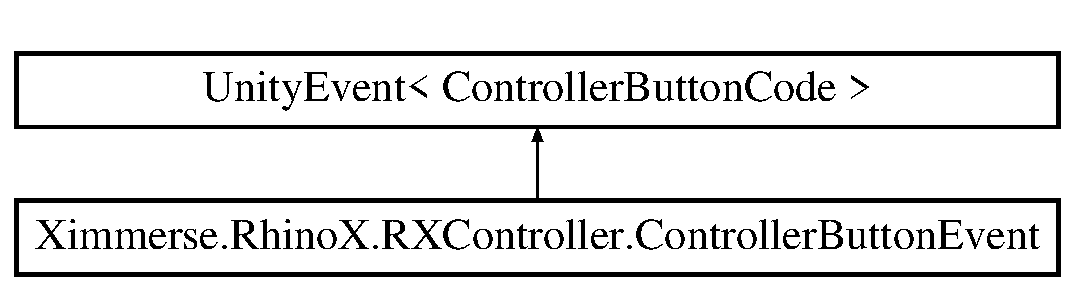
\includegraphics[height=2.000000cm]{class_ximmerse_1_1_rhino_x_1_1_r_x_controller_1_1_controller_button_event}
\end{center}
\end{figure}


The documentation for this class was generated from the following file\+:\begin{DoxyCompactItemize}
\item 
Event\+System/R\+X\+Controller.\+cs\end{DoxyCompactItemize}

\hypertarget{struct_ximmerse_1_1_rhino_x_1_1_controller_gyroscope}{}\section{Ximmerse.\+Rhino\+X.\+Controller\+Gyroscope Struct Reference}
\label{struct_ximmerse_1_1_rhino_x_1_1_controller_gyroscope}\index{Ximmerse.\+Rhino\+X.\+Controller\+Gyroscope@{Ximmerse.\+Rhino\+X.\+Controller\+Gyroscope}}


Controller gyroscope information  


\subsection*{Properties}
\begin{DoxyCompactItemize}
\item 
Quaternion \mbox{\hyperlink{struct_ximmerse_1_1_rhino_x_1_1_controller_gyroscope_a694963cea4f05271994cf1ffcaae5dec}{Rotation}}\hspace{0.3cm}{\ttfamily  \mbox{[}get, set\mbox{]}}
\begin{DoxyCompactList}\small\item\em Gets controller gyroscope rotation. \end{DoxyCompactList}\end{DoxyCompactItemize}


\subsection{Detailed Description}
Controller gyroscope information 



\subsection{Property Documentation}
\mbox{\Hypertarget{struct_ximmerse_1_1_rhino_x_1_1_controller_gyroscope_a694963cea4f05271994cf1ffcaae5dec}\label{struct_ximmerse_1_1_rhino_x_1_1_controller_gyroscope_a694963cea4f05271994cf1ffcaae5dec}} 
\index{Ximmerse\+::\+Rhino\+X\+::\+Controller\+Gyroscope@{Ximmerse\+::\+Rhino\+X\+::\+Controller\+Gyroscope}!Rotation@{Rotation}}
\index{Rotation@{Rotation}!Ximmerse\+::\+Rhino\+X\+::\+Controller\+Gyroscope@{Ximmerse\+::\+Rhino\+X\+::\+Controller\+Gyroscope}}
\subsubsection{\texorpdfstring{Rotation}{Rotation}}
{\footnotesize\ttfamily Quaternion Ximmerse.\+Rhino\+X.\+Controller\+Gyroscope.\+Rotation\hspace{0.3cm}{\ttfamily [get]}, {\ttfamily [set]}}



Gets controller gyroscope rotation. 

The rotation.

The documentation for this struct was generated from the following file\+:\begin{DoxyCompactItemize}
\item 
Event\+System/R\+X\+Controller.\+cs\end{DoxyCompactItemize}

\hypertarget{class_ximmerse_1_1_rhino_x_1_1_dynamic_target}{}\section{Ximmerse.\+Rhino\+X.\+Dynamic\+Target Class Reference}
\label{class_ximmerse_1_1_rhino_x_1_1_dynamic_target}\index{Ximmerse.\+Rhino\+X.\+Dynamic\+Target@{Ximmerse.\+Rhino\+X.\+Dynamic\+Target}}


Default trackable behaviour, updates trackable object\textquotesingle{}s transform at the head space per-\/frame.  


Inheritance diagram for Ximmerse.\+Rhino\+X.\+Dynamic\+Target\+:\begin{figure}[H]
\begin{center}
\leavevmode
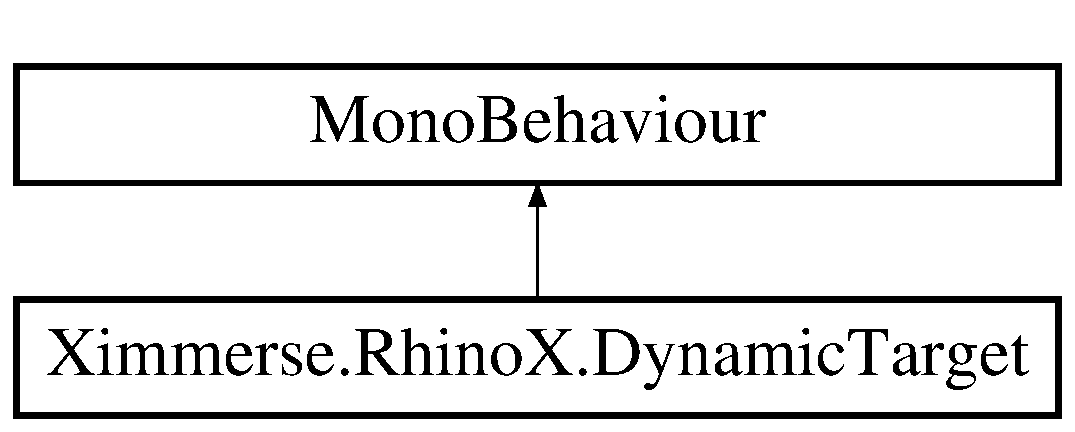
\includegraphics[height=2.000000cm]{class_ximmerse_1_1_rhino_x_1_1_dynamic_target}
\end{center}
\end{figure}
\subsection*{Properties}
\begin{DoxyCompactItemize}
\item 
\mbox{\Hypertarget{class_ximmerse_1_1_rhino_x_1_1_dynamic_target_afa6a6fdabf3e57d91d5945ae8f537aea}\label{class_ximmerse_1_1_rhino_x_1_1_dynamic_target_afa6a6fdabf3e57d91d5945ae8f537aea}} 
float {\bfseries Delay\+Time}\hspace{0.3cm}{\ttfamily  \mbox{[}get, set\mbox{]}}
\item 
\mbox{\Hypertarget{class_ximmerse_1_1_rhino_x_1_1_dynamic_target_acb8d72d226cf996cd674931aa87d89ed}\label{class_ximmerse_1_1_rhino_x_1_1_dynamic_target_acb8d72d226cf996cd674931aa87d89ed}} 
bool {\bfseries Yaw\+Only}\hspace{0.3cm}{\ttfamily  \mbox{[}get, set\mbox{]}}
\item 
Vector3 \mbox{\hyperlink{class_ximmerse_1_1_rhino_x_1_1_dynamic_target_a37e5698a43ecbe8551c95a4778498e1f}{Tilt}}\hspace{0.3cm}{\ttfamily  \mbox{[}get, set\mbox{]}}
\begin{DoxyCompactList}\small\item\em Gets or sets the tilt euler angle. \end{DoxyCompactList}\item 
bool \mbox{\hyperlink{class_ximmerse_1_1_rhino_x_1_1_dynamic_target_a09cea51d7c493761a0987036d2956865}{Debug\+View}}\hspace{0.3cm}{\ttfamily  \mbox{[}get, set\mbox{]}}
\begin{DoxyCompactList}\small\item\em Gets or sets a value indicating whether this T\+:\+Ximmerse.\+Rhino\+X.\+Dynamic\+Target debug view. \end{DoxyCompactList}\item 
Color \mbox{\hyperlink{class_ximmerse_1_1_rhino_x_1_1_dynamic_target_af798d3c901e13bc79c03c1044c95849b}{Debug\+Card\+Frame\+Color}}\hspace{0.3cm}{\ttfamily  \mbox{[}get, set\mbox{]}}
\begin{DoxyCompactList}\small\item\em Gets or sets the color of the color to draw debug card frame. \end{DoxyCompactList}\item 
Color \mbox{\hyperlink{class_ximmerse_1_1_rhino_x_1_1_dynamic_target_a5db410106585c9c1a96f5402be2779a4}{Debug\+Color\+\_\+\+Text}}\hspace{0.3cm}{\ttfamily  \mbox{[}get, set\mbox{]}}
\begin{DoxyCompactList}\small\item\em Gets or sets the debug color to draw text.. \end{DoxyCompactList}\item 
Debug\+Draw\+Type \mbox{\hyperlink{class_ximmerse_1_1_rhino_x_1_1_dynamic_target_a3d14c67bb9a13513f9227ccc7cf8d38d}{Draw\+Type}}\hspace{0.3cm}{\ttfamily  \mbox{[}get, set\mbox{]}}
\begin{DoxyCompactList}\small\item\em Gets or sets the type of the debug draw. \end{DoxyCompactList}\item 
bool \mbox{\hyperlink{class_ximmerse_1_1_rhino_x_1_1_dynamic_target_a5ef7419287f85eb97806cea82d617d01}{Print\+Detail\+Tracked\+Data}}\hspace{0.3cm}{\ttfamily  \mbox{[}get, set\mbox{]}}
\begin{DoxyCompactList}\small\item\em Gets or sets a value indicating whether this T\+:\+Ximmerse.\+Rhino\+X.\+Dynamic\+Target print detail tracked data. \end{DoxyCompactList}\item 
float \mbox{\hyperlink{class_ximmerse_1_1_rhino_x_1_1_dynamic_target_a6b87feb1464720270d2fdfd18966c933}{Debug\+Text\+Scale}}\hspace{0.3cm}{\ttfamily  \mbox{[}get, set\mbox{]}}
\begin{DoxyCompactList}\small\item\em Gets or sets the debug text scale. \end{DoxyCompactList}\end{DoxyCompactItemize}


\subsection{Detailed Description}
Default trackable behaviour, updates trackable object\textquotesingle{}s transform at the head space per-\/frame. 



\subsection{Property Documentation}
\mbox{\Hypertarget{class_ximmerse_1_1_rhino_x_1_1_dynamic_target_af798d3c901e13bc79c03c1044c95849b}\label{class_ximmerse_1_1_rhino_x_1_1_dynamic_target_af798d3c901e13bc79c03c1044c95849b}} 
\index{Ximmerse\+::\+Rhino\+X\+::\+Dynamic\+Target@{Ximmerse\+::\+Rhino\+X\+::\+Dynamic\+Target}!Debug\+Card\+Frame\+Color@{Debug\+Card\+Frame\+Color}}
\index{Debug\+Card\+Frame\+Color@{Debug\+Card\+Frame\+Color}!Ximmerse\+::\+Rhino\+X\+::\+Dynamic\+Target@{Ximmerse\+::\+Rhino\+X\+::\+Dynamic\+Target}}
\subsubsection{\texorpdfstring{Debug\+Card\+Frame\+Color}{DebugCardFrameColor}}
{\footnotesize\ttfamily Color Ximmerse.\+Rhino\+X.\+Dynamic\+Target.\+Debug\+Card\+Frame\+Color\hspace{0.3cm}{\ttfamily [get]}, {\ttfamily [set]}}



Gets or sets the color of the color to draw debug card frame. 

The color of the debug.\mbox{\Hypertarget{class_ximmerse_1_1_rhino_x_1_1_dynamic_target_a5db410106585c9c1a96f5402be2779a4}\label{class_ximmerse_1_1_rhino_x_1_1_dynamic_target_a5db410106585c9c1a96f5402be2779a4}} 
\index{Ximmerse\+::\+Rhino\+X\+::\+Dynamic\+Target@{Ximmerse\+::\+Rhino\+X\+::\+Dynamic\+Target}!Debug\+Color\+\_\+\+Text@{Debug\+Color\+\_\+\+Text}}
\index{Debug\+Color\+\_\+\+Text@{Debug\+Color\+\_\+\+Text}!Ximmerse\+::\+Rhino\+X\+::\+Dynamic\+Target@{Ximmerse\+::\+Rhino\+X\+::\+Dynamic\+Target}}
\subsubsection{\texorpdfstring{Debug\+Color\+\_\+\+Text}{DebugColor\_Text}}
{\footnotesize\ttfamily Color Ximmerse.\+Rhino\+X.\+Dynamic\+Target.\+Debug\+Color\+\_\+\+Text\hspace{0.3cm}{\ttfamily [get]}, {\ttfamily [set]}}



Gets or sets the debug color to draw text.. 

The debug color text.\mbox{\Hypertarget{class_ximmerse_1_1_rhino_x_1_1_dynamic_target_a6b87feb1464720270d2fdfd18966c933}\label{class_ximmerse_1_1_rhino_x_1_1_dynamic_target_a6b87feb1464720270d2fdfd18966c933}} 
\index{Ximmerse\+::\+Rhino\+X\+::\+Dynamic\+Target@{Ximmerse\+::\+Rhino\+X\+::\+Dynamic\+Target}!Debug\+Text\+Scale@{Debug\+Text\+Scale}}
\index{Debug\+Text\+Scale@{Debug\+Text\+Scale}!Ximmerse\+::\+Rhino\+X\+::\+Dynamic\+Target@{Ximmerse\+::\+Rhino\+X\+::\+Dynamic\+Target}}
\subsubsection{\texorpdfstring{Debug\+Text\+Scale}{DebugTextScale}}
{\footnotesize\ttfamily float Ximmerse.\+Rhino\+X.\+Dynamic\+Target.\+Debug\+Text\+Scale\hspace{0.3cm}{\ttfamily [get]}, {\ttfamily [set]}}



Gets or sets the debug text scale. 

The debug text scale.\mbox{\Hypertarget{class_ximmerse_1_1_rhino_x_1_1_dynamic_target_a09cea51d7c493761a0987036d2956865}\label{class_ximmerse_1_1_rhino_x_1_1_dynamic_target_a09cea51d7c493761a0987036d2956865}} 
\index{Ximmerse\+::\+Rhino\+X\+::\+Dynamic\+Target@{Ximmerse\+::\+Rhino\+X\+::\+Dynamic\+Target}!Debug\+View@{Debug\+View}}
\index{Debug\+View@{Debug\+View}!Ximmerse\+::\+Rhino\+X\+::\+Dynamic\+Target@{Ximmerse\+::\+Rhino\+X\+::\+Dynamic\+Target}}
\subsubsection{\texorpdfstring{Debug\+View}{DebugView}}
{\footnotesize\ttfamily bool Ximmerse.\+Rhino\+X.\+Dynamic\+Target.\+Debug\+View\hspace{0.3cm}{\ttfamily [get]}, {\ttfamily [set]}}



Gets or sets a value indicating whether this T\+:\+Ximmerse.\+Rhino\+X.\+Dynamic\+Target debug view. 

{\ttfamily true} if debug view; otherwise, {\ttfamily false}.\mbox{\Hypertarget{class_ximmerse_1_1_rhino_x_1_1_dynamic_target_a3d14c67bb9a13513f9227ccc7cf8d38d}\label{class_ximmerse_1_1_rhino_x_1_1_dynamic_target_a3d14c67bb9a13513f9227ccc7cf8d38d}} 
\index{Ximmerse\+::\+Rhino\+X\+::\+Dynamic\+Target@{Ximmerse\+::\+Rhino\+X\+::\+Dynamic\+Target}!Draw\+Type@{Draw\+Type}}
\index{Draw\+Type@{Draw\+Type}!Ximmerse\+::\+Rhino\+X\+::\+Dynamic\+Target@{Ximmerse\+::\+Rhino\+X\+::\+Dynamic\+Target}}
\subsubsection{\texorpdfstring{Draw\+Type}{DrawType}}
{\footnotesize\ttfamily Debug\+Draw\+Type Ximmerse.\+Rhino\+X.\+Dynamic\+Target.\+Draw\+Type\hspace{0.3cm}{\ttfamily [get]}, {\ttfamily [set]}}



Gets or sets the type of the debug draw. 

The type of the draw.\mbox{\Hypertarget{class_ximmerse_1_1_rhino_x_1_1_dynamic_target_a5ef7419287f85eb97806cea82d617d01}\label{class_ximmerse_1_1_rhino_x_1_1_dynamic_target_a5ef7419287f85eb97806cea82d617d01}} 
\index{Ximmerse\+::\+Rhino\+X\+::\+Dynamic\+Target@{Ximmerse\+::\+Rhino\+X\+::\+Dynamic\+Target}!Print\+Detail\+Tracked\+Data@{Print\+Detail\+Tracked\+Data}}
\index{Print\+Detail\+Tracked\+Data@{Print\+Detail\+Tracked\+Data}!Ximmerse\+::\+Rhino\+X\+::\+Dynamic\+Target@{Ximmerse\+::\+Rhino\+X\+::\+Dynamic\+Target}}
\subsubsection{\texorpdfstring{Print\+Detail\+Tracked\+Data}{PrintDetailTrackedData}}
{\footnotesize\ttfamily bool Ximmerse.\+Rhino\+X.\+Dynamic\+Target.\+Print\+Detail\+Tracked\+Data\hspace{0.3cm}{\ttfamily [get]}, {\ttfamily [set]}}



Gets or sets a value indicating whether this T\+:\+Ximmerse.\+Rhino\+X.\+Dynamic\+Target print detail tracked data. 

{\ttfamily true} if print detail tracked data; otherwise, {\ttfamily false}.\mbox{\Hypertarget{class_ximmerse_1_1_rhino_x_1_1_dynamic_target_a37e5698a43ecbe8551c95a4778498e1f}\label{class_ximmerse_1_1_rhino_x_1_1_dynamic_target_a37e5698a43ecbe8551c95a4778498e1f}} 
\index{Ximmerse\+::\+Rhino\+X\+::\+Dynamic\+Target@{Ximmerse\+::\+Rhino\+X\+::\+Dynamic\+Target}!Tilt@{Tilt}}
\index{Tilt@{Tilt}!Ximmerse\+::\+Rhino\+X\+::\+Dynamic\+Target@{Ximmerse\+::\+Rhino\+X\+::\+Dynamic\+Target}}
\subsubsection{\texorpdfstring{Tilt}{Tilt}}
{\footnotesize\ttfamily Vector3 Ximmerse.\+Rhino\+X.\+Dynamic\+Target.\+Tilt\hspace{0.3cm}{\ttfamily [get]}, {\ttfamily [set]}}



Gets or sets the tilt euler angle. 

The tilt.

The documentation for this class was generated from the following file\+:\begin{DoxyCompactItemize}
\item 
H\+L\+A\+P\+I/\+Public/Dynamic\+Target.\+cs\end{DoxyCompactItemize}

\hypertarget{class_ximmerse_1_1_rhino_x_1_1_ground_plane}{}\section{Ximmerse.\+Rhino\+X.\+Ground\+Plane Class Reference}
\label{class_ximmerse_1_1_rhino_x_1_1_ground_plane}\index{Ximmerse.\+Rhino\+X.\+Ground\+Plane@{Ximmerse.\+Rhino\+X.\+Ground\+Plane}}


Ground plane represents static trackable object placed on environment, to reposition head pose according to the relative pose between head and trackable object.  


Inheritance diagram for Ximmerse.\+Rhino\+X.\+Ground\+Plane\+:\begin{figure}[H]
\begin{center}
\leavevmode
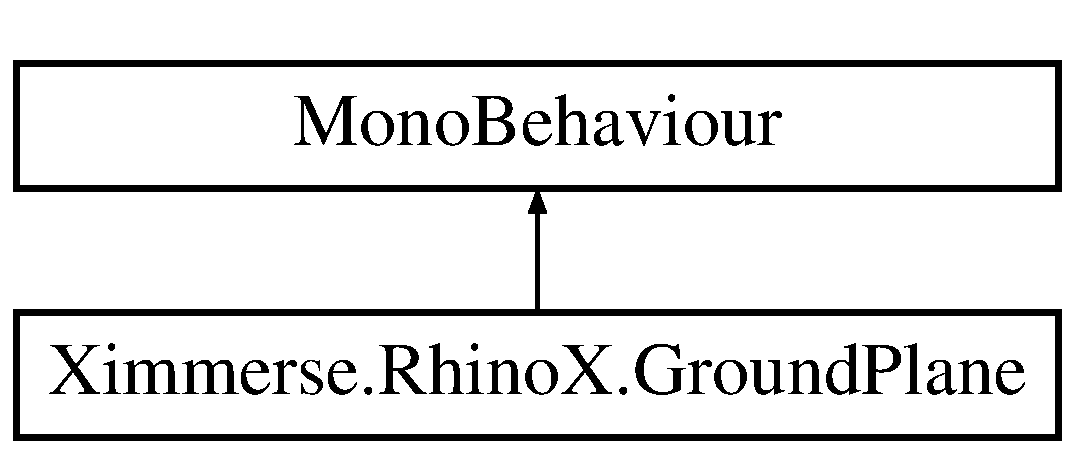
\includegraphics[height=2.000000cm]{class_ximmerse_1_1_rhino_x_1_1_ground_plane}
\end{center}
\end{figure}
\subsection*{Public Types}
\begin{DoxyCompactItemize}
\item 
enum \mbox{\hyperlink{class_ximmerse_1_1_rhino_x_1_1_ground_plane_a8813fd8673b953d9d9eb5e87b16cad14}{Recenter\+Mode}} \{ \mbox{\hyperlink{class_ximmerse_1_1_rhino_x_1_1_ground_plane_a8813fd8673b953d9d9eb5e87b16cad14ae7052705ca5b1918757966609990e511}{Recenter\+Mode.\+Everyframe}} = 0, 
\mbox{\hyperlink{class_ximmerse_1_1_rhino_x_1_1_ground_plane_a8813fd8673b953d9d9eb5e87b16cad14a8fcbeb1464e18e07dc95e57674102532}{Recenter\+Mode.\+Fixed\+Interval}} = 1, 
\mbox{\hyperlink{class_ximmerse_1_1_rhino_x_1_1_ground_plane_a8813fd8673b953d9d9eb5e87b16cad14a7aa380179987cdf970ad4a8ac6d81d46}{Recenter\+Mode.\+First\+Tracked}} = 2
 \}
\begin{DoxyCompactList}\small\item\em Recenter behaviour mode. \end{DoxyCompactList}\end{DoxyCompactItemize}
\subsection*{Properties}
\begin{DoxyCompactItemize}
\item 
\mbox{\hyperlink{class_ximmerse_1_1_rhino_x_1_1_ground_plane_a8813fd8673b953d9d9eb5e87b16cad14}{Recenter\+Mode}} \mbox{\hyperlink{class_ximmerse_1_1_rhino_x_1_1_ground_plane_a9d8f6a9a11b6f928eb2312dd829ddc80}{recenter\+Mode}}\hspace{0.3cm}{\ttfamily  \mbox{[}get, set\mbox{]}}
\begin{DoxyCompactList}\small\item\em Gets or sets the recenter mode. \end{DoxyCompactList}\item 
float \mbox{\hyperlink{class_ximmerse_1_1_rhino_x_1_1_ground_plane_a038a86a7608ce2283055c64b7c29848a}{Recenter\+Interval}}\hspace{0.3cm}{\ttfamily  \mbox{[}get, set\mbox{]}}
\begin{DoxyCompactList}\small\item\em Gets or sets the recenter interval. \end{DoxyCompactList}\item 
Vector3 \mbox{\hyperlink{class_ximmerse_1_1_rhino_x_1_1_ground_plane_a898f82c1d352c5f0749184d6fa346282}{Tilt\+Euler}}\hspace{0.3cm}{\ttfamily  \mbox{[}get, set\mbox{]}}
\begin{DoxyCompactList}\small\item\em Gets or sets the euler tilt. The world rotation of ground plane can be adjusted by this euler. \end{DoxyCompactList}\item 
float \mbox{\hyperlink{class_ximmerse_1_1_rhino_x_1_1_ground_plane_ad865efbe2157148db7f6ee7513b461b8}{V\+P\+U\+Frame\+Delay}}\hspace{0.3cm}{\ttfamily  \mbox{[}get, set\mbox{]}}
\begin{DoxyCompactList}\small\item\em Gets or sets the delay time from rendering to V\+PU. \end{DoxyCompactList}\item 
float \mbox{\hyperlink{class_ximmerse_1_1_rhino_x_1_1_ground_plane_aeb62f8cf91b1beb542a7f109ee15cc7d}{Min\+Tracked\+Distance}}\hspace{0.3cm}{\ttfamily  \mbox{[}get, set\mbox{]}}
\begin{DoxyCompactList}\small\item\em Gets or sets the minimum tracking distance to allow recenter. 可以发生对齐的最小追踪距离. \end{DoxyCompactList}\item 
float \mbox{\hyperlink{class_ximmerse_1_1_rhino_x_1_1_ground_plane_a9fdce85c8aa0f79d7a3bfd5e405690e6}{Max\+Tracked\+Distance}}\hspace{0.3cm}{\ttfamily  \mbox{[}get, set\mbox{]}}
\begin{DoxyCompactList}\small\item\em Gets or sets the max tracking distance to allow recenter. 可以发生对齐的最大追踪距离. \end{DoxyCompactList}\item 
float \mbox{\hyperlink{class_ximmerse_1_1_rhino_x_1_1_ground_plane_a17e5a8401d6fff9932ee9be50a63557d}{Min\+Error\+Head\+Distance}}\hspace{0.3cm}{\ttfamily  \mbox{[}get, set\mbox{]}}
\begin{DoxyCompactList}\small\item\em The minimum error head distance. 对齐时候允许头部对齐动作的最小距离. \end{DoxyCompactList}\item 
bool \mbox{\hyperlink{class_ximmerse_1_1_rhino_x_1_1_ground_plane_aae04f4e2f68e795bce517209568b90ef}{Debug\+View}}\hspace{0.3cm}{\ttfamily  \mbox{[}get, set\mbox{]}}
\begin{DoxyCompactList}\small\item\em Activates or deactivate debug view. \end{DoxyCompactList}\item 
float \mbox{\hyperlink{class_ximmerse_1_1_rhino_x_1_1_ground_plane_a2b83cdffdc6141b39c695a0588b19568}{Min\+Error\+Head\+Diff\+Angle}}\hspace{0.3cm}{\ttfamily  \mbox{[}get, set\mbox{]}}
\begin{DoxyCompactList}\small\item\em Gets or sets the minimum allow head diff angle to recenter. \end{DoxyCompactList}\item 
\mbox{\Hypertarget{class_ximmerse_1_1_rhino_x_1_1_ground_plane_a88437781a9762727b2cd7ea8f931bdcb}\label{class_ximmerse_1_1_rhino_x_1_1_ground_plane_a88437781a9762727b2cd7ea8f931bdcb}} 
Color {\bfseries Debug\+Color\+\_\+\+Frame}\hspace{0.3cm}{\ttfamily  \mbox{[}get, set\mbox{]}}
\item 
\mbox{\Hypertarget{class_ximmerse_1_1_rhino_x_1_1_ground_plane_a9d37c7e36bbb00afc848ad540d2ff1e8}\label{class_ximmerse_1_1_rhino_x_1_1_ground_plane_a9d37c7e36bbb00afc848ad540d2ff1e8}} 
Color {\bfseries Debug\+Color\+\_\+\+Text}\hspace{0.3cm}{\ttfamily  \mbox{[}get, set\mbox{]}}
\item 
\mbox{\Hypertarget{class_ximmerse_1_1_rhino_x_1_1_ground_plane_af723d66a4c3fff91ef5033d667ef2436}\label{class_ximmerse_1_1_rhino_x_1_1_ground_plane_af723d66a4c3fff91ef5033d667ef2436}} 
bool {\bfseries Print\+Detail\+Tracked\+Data}\hspace{0.3cm}{\ttfamily  \mbox{[}get, set\mbox{]}}
\item 
\mbox{\Hypertarget{class_ximmerse_1_1_rhino_x_1_1_ground_plane_af70f6507f27354b7e614d3a581466920}\label{class_ximmerse_1_1_rhino_x_1_1_ground_plane_af70f6507f27354b7e614d3a581466920}} 
float {\bfseries Debug\+Text\+Scale}\hspace{0.3cm}{\ttfamily  \mbox{[}get, set\mbox{]}}
\end{DoxyCompactItemize}


\subsection{Detailed Description}
Ground plane represents static trackable object placed on environment, to reposition head pose according to the relative pose between head and trackable object. 



\subsection{Member Enumeration Documentation}
\mbox{\Hypertarget{class_ximmerse_1_1_rhino_x_1_1_ground_plane_a8813fd8673b953d9d9eb5e87b16cad14}\label{class_ximmerse_1_1_rhino_x_1_1_ground_plane_a8813fd8673b953d9d9eb5e87b16cad14}} 
\index{Ximmerse\+::\+Rhino\+X\+::\+Ground\+Plane@{Ximmerse\+::\+Rhino\+X\+::\+Ground\+Plane}!Recenter\+Mode@{Recenter\+Mode}}
\index{Recenter\+Mode@{Recenter\+Mode}!Ximmerse\+::\+Rhino\+X\+::\+Ground\+Plane@{Ximmerse\+::\+Rhino\+X\+::\+Ground\+Plane}}
\subsubsection{\texorpdfstring{Recenter\+Mode}{RecenterMode}}
{\footnotesize\ttfamily enum \mbox{\hyperlink{class_ximmerse_1_1_rhino_x_1_1_ground_plane_a8813fd8673b953d9d9eb5e87b16cad14}{Ximmerse.\+Rhino\+X.\+Ground\+Plane.\+Recenter\+Mode}}\hspace{0.3cm}{\ttfamily [strong]}}



Recenter behaviour mode. 

\begin{DoxyEnumFields}{Enumerator}
\raisebox{\heightof{T}}[0pt][0pt]{\index{Everyframe@{Everyframe}!Ximmerse\+::\+Rhino\+X\+::\+Ground\+Plane@{Ximmerse\+::\+Rhino\+X\+::\+Ground\+Plane}}\index{Ximmerse\+::\+Rhino\+X\+::\+Ground\+Plane@{Ximmerse\+::\+Rhino\+X\+::\+Ground\+Plane}!Everyframe@{Everyframe}}}\mbox{\Hypertarget{class_ximmerse_1_1_rhino_x_1_1_ground_plane_a8813fd8673b953d9d9eb5e87b16cad14ae7052705ca5b1918757966609990e511}\label{class_ximmerse_1_1_rhino_x_1_1_ground_plane_a8813fd8673b953d9d9eb5e87b16cad14ae7052705ca5b1918757966609990e511}} 
Everyframe&Tries to recenter head everyframe, as long as the ground plane object is tracked. This is the default mode; \\
\hline

\raisebox{\heightof{T}}[0pt][0pt]{\index{Fixed\+Interval@{Fixed\+Interval}!Ximmerse\+::\+Rhino\+X\+::\+Ground\+Plane@{Ximmerse\+::\+Rhino\+X\+::\+Ground\+Plane}}\index{Ximmerse\+::\+Rhino\+X\+::\+Ground\+Plane@{Ximmerse\+::\+Rhino\+X\+::\+Ground\+Plane}!Fixed\+Interval@{Fixed\+Interval}}}\mbox{\Hypertarget{class_ximmerse_1_1_rhino_x_1_1_ground_plane_a8813fd8673b953d9d9eb5e87b16cad14a8fcbeb1464e18e07dc95e57674102532}\label{class_ximmerse_1_1_rhino_x_1_1_ground_plane_a8813fd8673b953d9d9eb5e87b16cad14a8fcbeb1464e18e07dc95e57674102532}} 
Fixed\+Interval&Try to recenter in a fixed time interval. \\
\hline

\raisebox{\heightof{T}}[0pt][0pt]{\index{First\+Tracked@{First\+Tracked}!Ximmerse\+::\+Rhino\+X\+::\+Ground\+Plane@{Ximmerse\+::\+Rhino\+X\+::\+Ground\+Plane}}\index{Ximmerse\+::\+Rhino\+X\+::\+Ground\+Plane@{Ximmerse\+::\+Rhino\+X\+::\+Ground\+Plane}!First\+Tracked@{First\+Tracked}}}\mbox{\Hypertarget{class_ximmerse_1_1_rhino_x_1_1_ground_plane_a8813fd8673b953d9d9eb5e87b16cad14a7aa380179987cdf970ad4a8ac6d81d46}\label{class_ximmerse_1_1_rhino_x_1_1_ground_plane_a8813fd8673b953d9d9eb5e87b16cad14a7aa380179987cdf970ad4a8ac6d81d46}} 
First\+Tracked&Recenter head at the first frame when the ground plane object is tracked, then never recenter again until the ground plane is lost tracked and become visible again. \\
\hline

\end{DoxyEnumFields}


\subsection{Property Documentation}
\mbox{\Hypertarget{class_ximmerse_1_1_rhino_x_1_1_ground_plane_aae04f4e2f68e795bce517209568b90ef}\label{class_ximmerse_1_1_rhino_x_1_1_ground_plane_aae04f4e2f68e795bce517209568b90ef}} 
\index{Ximmerse\+::\+Rhino\+X\+::\+Ground\+Plane@{Ximmerse\+::\+Rhino\+X\+::\+Ground\+Plane}!Debug\+View@{Debug\+View}}
\index{Debug\+View@{Debug\+View}!Ximmerse\+::\+Rhino\+X\+::\+Ground\+Plane@{Ximmerse\+::\+Rhino\+X\+::\+Ground\+Plane}}
\subsubsection{\texorpdfstring{Debug\+View}{DebugView}}
{\footnotesize\ttfamily bool Ximmerse.\+Rhino\+X.\+Ground\+Plane.\+Debug\+View\hspace{0.3cm}{\ttfamily [get]}, {\ttfamily [set]}}



Activates or deactivate debug view. 

{\ttfamily true} if debug view; otherwise, {\ttfamily false}.\mbox{\Hypertarget{class_ximmerse_1_1_rhino_x_1_1_ground_plane_a9fdce85c8aa0f79d7a3bfd5e405690e6}\label{class_ximmerse_1_1_rhino_x_1_1_ground_plane_a9fdce85c8aa0f79d7a3bfd5e405690e6}} 
\index{Ximmerse\+::\+Rhino\+X\+::\+Ground\+Plane@{Ximmerse\+::\+Rhino\+X\+::\+Ground\+Plane}!Max\+Tracked\+Distance@{Max\+Tracked\+Distance}}
\index{Max\+Tracked\+Distance@{Max\+Tracked\+Distance}!Ximmerse\+::\+Rhino\+X\+::\+Ground\+Plane@{Ximmerse\+::\+Rhino\+X\+::\+Ground\+Plane}}
\subsubsection{\texorpdfstring{Max\+Tracked\+Distance}{MaxTrackedDistance}}
{\footnotesize\ttfamily float Ximmerse.\+Rhino\+X.\+Ground\+Plane.\+Max\+Tracked\+Distance\hspace{0.3cm}{\ttfamily [get]}, {\ttfamily [set]}}



Gets or sets the max tracking distance to allow recenter. 可以发生对齐的最大追踪距离. 

The max recenter distance.\mbox{\Hypertarget{class_ximmerse_1_1_rhino_x_1_1_ground_plane_a2b83cdffdc6141b39c695a0588b19568}\label{class_ximmerse_1_1_rhino_x_1_1_ground_plane_a2b83cdffdc6141b39c695a0588b19568}} 
\index{Ximmerse\+::\+Rhino\+X\+::\+Ground\+Plane@{Ximmerse\+::\+Rhino\+X\+::\+Ground\+Plane}!Min\+Error\+Head\+Diff\+Angle@{Min\+Error\+Head\+Diff\+Angle}}
\index{Min\+Error\+Head\+Diff\+Angle@{Min\+Error\+Head\+Diff\+Angle}!Ximmerse\+::\+Rhino\+X\+::\+Ground\+Plane@{Ximmerse\+::\+Rhino\+X\+::\+Ground\+Plane}}
\subsubsection{\texorpdfstring{Min\+Error\+Head\+Diff\+Angle}{MinErrorHeadDiffAngle}}
{\footnotesize\ttfamily float Ximmerse.\+Rhino\+X.\+Ground\+Plane.\+Min\+Error\+Head\+Diff\+Angle\hspace{0.3cm}{\ttfamily [get]}, {\ttfamily [set]}}



Gets or sets the minimum allow head diff angle to recenter. 

The minimum error head diff angle.\mbox{\Hypertarget{class_ximmerse_1_1_rhino_x_1_1_ground_plane_a17e5a8401d6fff9932ee9be50a63557d}\label{class_ximmerse_1_1_rhino_x_1_1_ground_plane_a17e5a8401d6fff9932ee9be50a63557d}} 
\index{Ximmerse\+::\+Rhino\+X\+::\+Ground\+Plane@{Ximmerse\+::\+Rhino\+X\+::\+Ground\+Plane}!Min\+Error\+Head\+Distance@{Min\+Error\+Head\+Distance}}
\index{Min\+Error\+Head\+Distance@{Min\+Error\+Head\+Distance}!Ximmerse\+::\+Rhino\+X\+::\+Ground\+Plane@{Ximmerse\+::\+Rhino\+X\+::\+Ground\+Plane}}
\subsubsection{\texorpdfstring{Min\+Error\+Head\+Distance}{MinErrorHeadDistance}}
{\footnotesize\ttfamily float Ximmerse.\+Rhino\+X.\+Ground\+Plane.\+Min\+Error\+Head\+Distance\hspace{0.3cm}{\ttfamily [get]}, {\ttfamily [set]}}



The minimum error head distance. 对齐时候允许头部对齐动作的最小距离. 

The minimum error head span.\mbox{\Hypertarget{class_ximmerse_1_1_rhino_x_1_1_ground_plane_aeb62f8cf91b1beb542a7f109ee15cc7d}\label{class_ximmerse_1_1_rhino_x_1_1_ground_plane_aeb62f8cf91b1beb542a7f109ee15cc7d}} 
\index{Ximmerse\+::\+Rhino\+X\+::\+Ground\+Plane@{Ximmerse\+::\+Rhino\+X\+::\+Ground\+Plane}!Min\+Tracked\+Distance@{Min\+Tracked\+Distance}}
\index{Min\+Tracked\+Distance@{Min\+Tracked\+Distance}!Ximmerse\+::\+Rhino\+X\+::\+Ground\+Plane@{Ximmerse\+::\+Rhino\+X\+::\+Ground\+Plane}}
\subsubsection{\texorpdfstring{Min\+Tracked\+Distance}{MinTrackedDistance}}
{\footnotesize\ttfamily float Ximmerse.\+Rhino\+X.\+Ground\+Plane.\+Min\+Tracked\+Distance\hspace{0.3cm}{\ttfamily [get]}, {\ttfamily [set]}}



Gets or sets the minimum tracking distance to allow recenter. 可以发生对齐的最小追踪距离. 

The minimum recenter distance.\mbox{\Hypertarget{class_ximmerse_1_1_rhino_x_1_1_ground_plane_a038a86a7608ce2283055c64b7c29848a}\label{class_ximmerse_1_1_rhino_x_1_1_ground_plane_a038a86a7608ce2283055c64b7c29848a}} 
\index{Ximmerse\+::\+Rhino\+X\+::\+Ground\+Plane@{Ximmerse\+::\+Rhino\+X\+::\+Ground\+Plane}!Recenter\+Interval@{Recenter\+Interval}}
\index{Recenter\+Interval@{Recenter\+Interval}!Ximmerse\+::\+Rhino\+X\+::\+Ground\+Plane@{Ximmerse\+::\+Rhino\+X\+::\+Ground\+Plane}}
\subsubsection{\texorpdfstring{Recenter\+Interval}{RecenterInterval}}
{\footnotesize\ttfamily float Ximmerse.\+Rhino\+X.\+Ground\+Plane.\+Recenter\+Interval\hspace{0.3cm}{\ttfamily [get]}, {\ttfamily [set]}}



Gets or sets the recenter interval. 

The recenter scanning interval.\mbox{\Hypertarget{class_ximmerse_1_1_rhino_x_1_1_ground_plane_a9d8f6a9a11b6f928eb2312dd829ddc80}\label{class_ximmerse_1_1_rhino_x_1_1_ground_plane_a9d8f6a9a11b6f928eb2312dd829ddc80}} 
\index{Ximmerse\+::\+Rhino\+X\+::\+Ground\+Plane@{Ximmerse\+::\+Rhino\+X\+::\+Ground\+Plane}!recenter\+Mode@{recenter\+Mode}}
\index{recenter\+Mode@{recenter\+Mode}!Ximmerse\+::\+Rhino\+X\+::\+Ground\+Plane@{Ximmerse\+::\+Rhino\+X\+::\+Ground\+Plane}}
\subsubsection{\texorpdfstring{recenter\+Mode}{recenterMode}}
{\footnotesize\ttfamily \mbox{\hyperlink{class_ximmerse_1_1_rhino_x_1_1_ground_plane_a8813fd8673b953d9d9eb5e87b16cad14}{Recenter\+Mode}} Ximmerse.\+Rhino\+X.\+Ground\+Plane.\+recenter\+Mode\hspace{0.3cm}{\ttfamily [get]}, {\ttfamily [set]}}



Gets or sets the recenter mode. 

The recenter mode.\mbox{\Hypertarget{class_ximmerse_1_1_rhino_x_1_1_ground_plane_a898f82c1d352c5f0749184d6fa346282}\label{class_ximmerse_1_1_rhino_x_1_1_ground_plane_a898f82c1d352c5f0749184d6fa346282}} 
\index{Ximmerse\+::\+Rhino\+X\+::\+Ground\+Plane@{Ximmerse\+::\+Rhino\+X\+::\+Ground\+Plane}!Tilt\+Euler@{Tilt\+Euler}}
\index{Tilt\+Euler@{Tilt\+Euler}!Ximmerse\+::\+Rhino\+X\+::\+Ground\+Plane@{Ximmerse\+::\+Rhino\+X\+::\+Ground\+Plane}}
\subsubsection{\texorpdfstring{Tilt\+Euler}{TiltEuler}}
{\footnotesize\ttfamily Vector3 Ximmerse.\+Rhino\+X.\+Ground\+Plane.\+Tilt\+Euler\hspace{0.3cm}{\ttfamily [get]}, {\ttfamily [set]}}



Gets or sets the euler tilt. The world rotation of ground plane can be adjusted by this euler. 

The euler offset.\mbox{\Hypertarget{class_ximmerse_1_1_rhino_x_1_1_ground_plane_ad865efbe2157148db7f6ee7513b461b8}\label{class_ximmerse_1_1_rhino_x_1_1_ground_plane_ad865efbe2157148db7f6ee7513b461b8}} 
\index{Ximmerse\+::\+Rhino\+X\+::\+Ground\+Plane@{Ximmerse\+::\+Rhino\+X\+::\+Ground\+Plane}!V\+P\+U\+Frame\+Delay@{V\+P\+U\+Frame\+Delay}}
\index{V\+P\+U\+Frame\+Delay@{V\+P\+U\+Frame\+Delay}!Ximmerse\+::\+Rhino\+X\+::\+Ground\+Plane@{Ximmerse\+::\+Rhino\+X\+::\+Ground\+Plane}}
\subsubsection{\texorpdfstring{V\+P\+U\+Frame\+Delay}{VPUFrameDelay}}
{\footnotesize\ttfamily float Ximmerse.\+Rhino\+X.\+Ground\+Plane.\+V\+P\+U\+Frame\+Delay\hspace{0.3cm}{\ttfamily [get]}, {\ttfamily [set]}}



Gets or sets the delay time from rendering to V\+PU. 

The backward time.

The documentation for this class was generated from the following file\+:\begin{DoxyCompactItemize}
\item 
Ground\+Plane.\+cs\end{DoxyCompactItemize}

\hypertarget{class_ximmerse_1_1_rhino_x_1_1_object_tracking_profile}{}\section{Ximmerse.\+Rhino\+X.\+Object\+Tracking\+Profile Class Reference}
\label{class_ximmerse_1_1_rhino_x_1_1_object_tracking_profile}\index{Ximmerse.\+Rhino\+X.\+Object\+Tracking\+Profile@{Ximmerse.\+Rhino\+X.\+Object\+Tracking\+Profile}}
Inheritance diagram for Ximmerse.\+Rhino\+X.\+Object\+Tracking\+Profile\+:\begin{figure}[H]
\begin{center}
\leavevmode
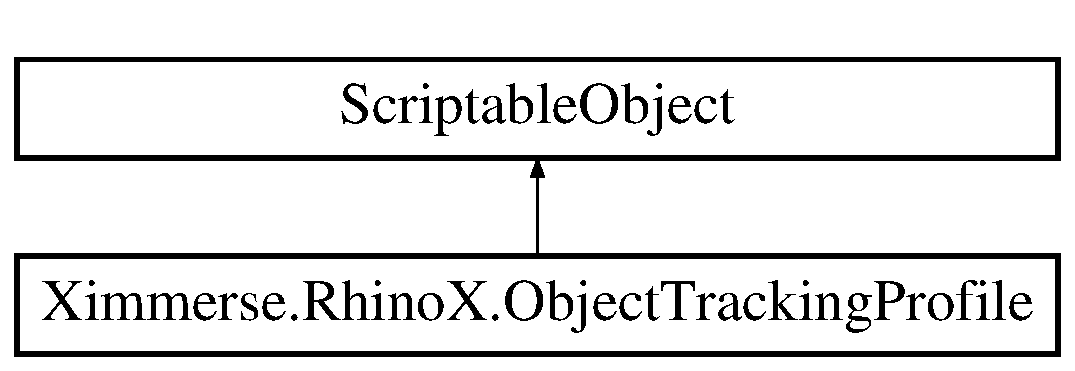
\includegraphics[height=2.000000cm]{class_ximmerse_1_1_rhino_x_1_1_object_tracking_profile}
\end{center}
\end{figure}
\subsection*{Classes}
\begin{DoxyCompactItemize}
\item 
class \mbox{\hyperlink{class_ximmerse_1_1_rhino_x_1_1_object_tracking_profile_1_1_tracking_items}{Tracking\+Items}}
\end{DoxyCompactItemize}
\subsection*{Public Member Functions}
\begin{DoxyCompactItemize}
\item 
void \mbox{\hyperlink{class_ximmerse_1_1_rhino_x_1_1_object_tracking_profile_a73cba033e2017accd3f607514ccf5935}{Add}} (string json\+Name, Unity\+Engine.\+Object json\+Object, string json\+Content)
\begin{DoxyCompactList}\small\item\em Adds a tracking item. \end{DoxyCompactList}\item 
void \mbox{\hyperlink{class_ximmerse_1_1_rhino_x_1_1_object_tracking_profile_a7096567a6cc3599254f38f73aebc3b09}{Remove}} (int Index)
\begin{DoxyCompactList}\small\item\em Removes the tracking items at the specific item. \end{DoxyCompactList}\item 
\mbox{\Hypertarget{class_ximmerse_1_1_rhino_x_1_1_object_tracking_profile_a1b298818407574a90fdd814b64a1108d}\label{class_ximmerse_1_1_rhino_x_1_1_object_tracking_profile_a1b298818407574a90fdd814b64a1108d}} 
void {\bfseries On\+Validate\+Self} ()
\end{DoxyCompactItemize}
\subsection*{Public Attributes}
\begin{DoxyCompactItemize}
\item 
\mbox{\Hypertarget{class_ximmerse_1_1_rhino_x_1_1_object_tracking_profile_a466e497ac9077bf261eb270b5a41f9f1}\label{class_ximmerse_1_1_rhino_x_1_1_object_tracking_profile_a466e497ac9077bf261eb270b5a41f9f1}} 
string {\bfseries Description}
\end{DoxyCompactItemize}
\subsection*{Properties}
\begin{DoxyCompactItemize}
\item 
bool \mbox{\hyperlink{class_ximmerse_1_1_rhino_x_1_1_object_tracking_profile_a3749a2ba2e7a79434c61475897b8d664}{Is\+Loaded}}\hspace{0.3cm}{\ttfamily  \mbox{[}get, set\mbox{]}}
\begin{DoxyCompactList}\small\item\em Has the tracking profile loaded by tracking system ? \end{DoxyCompactList}\item 
\mbox{\hyperlink{class_ximmerse_1_1_rhino_x_1_1_object_tracking_profile_1_1_tracking_items}{Tracking\+Items}} \mbox{[}$\,$\mbox{]} \mbox{\hyperlink{class_ximmerse_1_1_rhino_x_1_1_object_tracking_profile_ad9d2e13ef6fdf8e901f7ee53cf42a7d3}{tracking\+Items}}\hspace{0.3cm}{\ttfamily  \mbox{[}get\mbox{]}}
\begin{DoxyCompactList}\small\item\em Gets the tracking items. \end{DoxyCompactList}\end{DoxyCompactItemize}


\subsection{Member Function Documentation}
\mbox{\Hypertarget{class_ximmerse_1_1_rhino_x_1_1_object_tracking_profile_a73cba033e2017accd3f607514ccf5935}\label{class_ximmerse_1_1_rhino_x_1_1_object_tracking_profile_a73cba033e2017accd3f607514ccf5935}} 
\index{Ximmerse\+::\+Rhino\+X\+::\+Object\+Tracking\+Profile@{Ximmerse\+::\+Rhino\+X\+::\+Object\+Tracking\+Profile}!Add@{Add}}
\index{Add@{Add}!Ximmerse\+::\+Rhino\+X\+::\+Object\+Tracking\+Profile@{Ximmerse\+::\+Rhino\+X\+::\+Object\+Tracking\+Profile}}
\subsubsection{\texorpdfstring{Add()}{Add()}}
{\footnotesize\ttfamily void Ximmerse.\+Rhino\+X.\+Object\+Tracking\+Profile.\+Add (\begin{DoxyParamCaption}\item[{string}]{json\+Name,  }\item[{Unity\+Engine.\+Object}]{json\+Object,  }\item[{string}]{json\+Content }\end{DoxyParamCaption})\hspace{0.3cm}{\ttfamily [inline]}}



Adds a tracking item. 


\begin{DoxyParams}{Parameters}
{\em json\+Name} & Json name \+: the tracking json profile\textquotesingle{}s name\\
\hline
{\em json\+Object} & Json object \+: the tracking json object\textquotesingle{}s reference in your project asset. If you\textquotesingle{}re calling this A\+PI at runtime, json\+Object could be null. If you\textquotesingle{}re calling this A\+PI at unity editor, json\+Object should not be \mbox{\hyperlink{}{.}} \\
\hline
\end{DoxyParams}
\mbox{\Hypertarget{class_ximmerse_1_1_rhino_x_1_1_object_tracking_profile_a7096567a6cc3599254f38f73aebc3b09}\label{class_ximmerse_1_1_rhino_x_1_1_object_tracking_profile_a7096567a6cc3599254f38f73aebc3b09}} 
\index{Ximmerse\+::\+Rhino\+X\+::\+Object\+Tracking\+Profile@{Ximmerse\+::\+Rhino\+X\+::\+Object\+Tracking\+Profile}!Remove@{Remove}}
\index{Remove@{Remove}!Ximmerse\+::\+Rhino\+X\+::\+Object\+Tracking\+Profile@{Ximmerse\+::\+Rhino\+X\+::\+Object\+Tracking\+Profile}}
\subsubsection{\texorpdfstring{Remove()}{Remove()}}
{\footnotesize\ttfamily void Ximmerse.\+Rhino\+X.\+Object\+Tracking\+Profile.\+Remove (\begin{DoxyParamCaption}\item[{int}]{Index }\end{DoxyParamCaption})\hspace{0.3cm}{\ttfamily [inline]}}



Removes the tracking items at the specific item. 


\begin{DoxyParams}{Parameters}
{\em Index} & Index.\\
\hline
\end{DoxyParams}


\subsection{Property Documentation}
\mbox{\Hypertarget{class_ximmerse_1_1_rhino_x_1_1_object_tracking_profile_a3749a2ba2e7a79434c61475897b8d664}\label{class_ximmerse_1_1_rhino_x_1_1_object_tracking_profile_a3749a2ba2e7a79434c61475897b8d664}} 
\index{Ximmerse\+::\+Rhino\+X\+::\+Object\+Tracking\+Profile@{Ximmerse\+::\+Rhino\+X\+::\+Object\+Tracking\+Profile}!Is\+Loaded@{Is\+Loaded}}
\index{Is\+Loaded@{Is\+Loaded}!Ximmerse\+::\+Rhino\+X\+::\+Object\+Tracking\+Profile@{Ximmerse\+::\+Rhino\+X\+::\+Object\+Tracking\+Profile}}
\subsubsection{\texorpdfstring{Is\+Loaded}{IsLoaded}}
{\footnotesize\ttfamily bool Ximmerse.\+Rhino\+X.\+Object\+Tracking\+Profile.\+Is\+Loaded\hspace{0.3cm}{\ttfamily [get]}, {\ttfamily [set]}}



Has the tracking profile loaded by tracking system ? 

{\ttfamily true} if is loaded; otherwise, {\ttfamily false}.\mbox{\Hypertarget{class_ximmerse_1_1_rhino_x_1_1_object_tracking_profile_ad9d2e13ef6fdf8e901f7ee53cf42a7d3}\label{class_ximmerse_1_1_rhino_x_1_1_object_tracking_profile_ad9d2e13ef6fdf8e901f7ee53cf42a7d3}} 
\index{Ximmerse\+::\+Rhino\+X\+::\+Object\+Tracking\+Profile@{Ximmerse\+::\+Rhino\+X\+::\+Object\+Tracking\+Profile}!tracking\+Items@{tracking\+Items}}
\index{tracking\+Items@{tracking\+Items}!Ximmerse\+::\+Rhino\+X\+::\+Object\+Tracking\+Profile@{Ximmerse\+::\+Rhino\+X\+::\+Object\+Tracking\+Profile}}
\subsubsection{\texorpdfstring{tracking\+Items}{trackingItems}}
{\footnotesize\ttfamily \mbox{\hyperlink{class_ximmerse_1_1_rhino_x_1_1_object_tracking_profile_1_1_tracking_items}{Tracking\+Items}} \mbox{[}$\,$\mbox{]} Ximmerse.\+Rhino\+X.\+Object\+Tracking\+Profile.\+tracking\+Items\hspace{0.3cm}{\ttfamily [get]}}



Gets the tracking items. 

The tracking items.

The documentation for this class was generated from the following file\+:\begin{DoxyCompactItemize}
\item 
Object\+Tracking\+Profile.\+cs\end{DoxyCompactItemize}

\hypertarget{class_ximmerse_1_1_rhino_x_1_1_overlay}{}\section{Ximmerse.\+Rhino\+X.\+Overlay Class Reference}
\label{class_ximmerse_1_1_rhino_x_1_1_overlay}\index{Ximmerse.\+Rhino\+X.\+Overlay@{Ximmerse.\+Rhino\+X.\+Overlay}}


\mbox{\hyperlink{class_ximmerse_1_1_rhino_x_1_1_overlay}{Overlay}} \+: scripts for overlay rendering.  


Inheritance diagram for Ximmerse.\+Rhino\+X.\+Overlay\+:\begin{figure}[H]
\begin{center}
\leavevmode
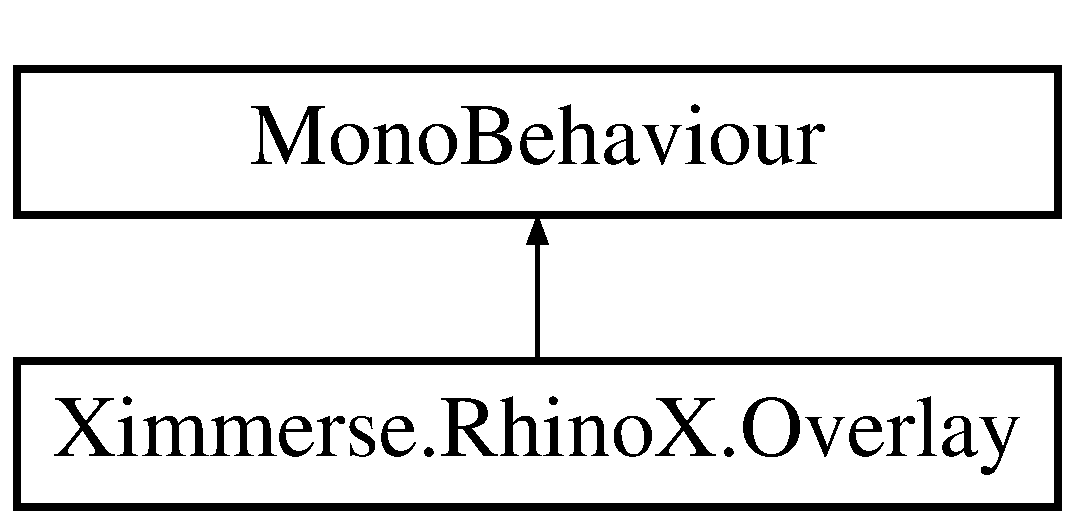
\includegraphics[height=2.000000cm]{class_ximmerse_1_1_rhino_x_1_1_overlay}
\end{center}
\end{figure}
\subsection*{Public Member Functions}
\begin{DoxyCompactItemize}
\item 
void \mbox{\hyperlink{class_ximmerse_1_1_rhino_x_1_1_overlay_a4fffeab006cc47fe53a3dbe2a4df7331}{Reset\+Overlay\+Clips}} ()
\begin{DoxyCompactList}\small\item\em Resets the overlay clips rect to full screen. \end{DoxyCompactList}\end{DoxyCompactItemize}
\subsection*{Properties}
\begin{DoxyCompactItemize}
\item 
Texture \mbox{\hyperlink{class_ximmerse_1_1_rhino_x_1_1_overlay_a33625bf90415d02965199b48bbaec4cc}{Image\+Texture}}\hspace{0.3cm}{\ttfamily  \mbox{[}get, set\mbox{]}}
\begin{DoxyCompactList}\small\item\em Gets or sets the image texture for overlay rendering. \end{DoxyCompactList}\item 
Transform \mbox{\hyperlink{class_ximmerse_1_1_rhino_x_1_1_overlay_a146fe73ef50033f83d4eac7354dded8e}{Image\+Transform}}\hspace{0.3cm}{\ttfamily  \mbox{[}get, set\mbox{]}}
\begin{DoxyCompactList}\small\item\em Gets or sets the image transform for overlay rendering binds to. \end{DoxyCompactList}\end{DoxyCompactItemize}


\subsection{Detailed Description}
\mbox{\hyperlink{class_ximmerse_1_1_rhino_x_1_1_overlay}{Overlay}} \+: scripts for overlay rendering. 



\subsection{Member Function Documentation}
\mbox{\Hypertarget{class_ximmerse_1_1_rhino_x_1_1_overlay_a4fffeab006cc47fe53a3dbe2a4df7331}\label{class_ximmerse_1_1_rhino_x_1_1_overlay_a4fffeab006cc47fe53a3dbe2a4df7331}} 
\index{Ximmerse\+::\+Rhino\+X\+::\+Overlay@{Ximmerse\+::\+Rhino\+X\+::\+Overlay}!Reset\+Overlay\+Clips@{Reset\+Overlay\+Clips}}
\index{Reset\+Overlay\+Clips@{Reset\+Overlay\+Clips}!Ximmerse\+::\+Rhino\+X\+::\+Overlay@{Ximmerse\+::\+Rhino\+X\+::\+Overlay}}
\subsubsection{\texorpdfstring{Reset\+Overlay\+Clips()}{ResetOverlayClips()}}
{\footnotesize\ttfamily void Ximmerse.\+Rhino\+X.\+Overlay.\+Reset\+Overlay\+Clips (\begin{DoxyParamCaption}{ }\end{DoxyParamCaption})\hspace{0.3cm}{\ttfamily [inline]}}



Resets the overlay clips rect to full screen. 

clip\+Lower\+Left = new Vector4(-\/1, -\/1, 0, 1); clip\+Upper\+Left = new Vector4(-\/1, 1, 0, 1); clip\+Upper\+Right = new Vector4(1, 1, 0, 1); clip\+Lower\+Right = new Vector4(1, -\/1, 0, 1);

uv\+Lower\+Left = new Vector2(0, 0); uv\+Upper\+Left = new Vector2(0, 1); uv\+Upper\+Right = new Vector2(1, 1); uv\+Lower\+Right = new Vector2(1, 0);

\subsection{Property Documentation}
\mbox{\Hypertarget{class_ximmerse_1_1_rhino_x_1_1_overlay_a33625bf90415d02965199b48bbaec4cc}\label{class_ximmerse_1_1_rhino_x_1_1_overlay_a33625bf90415d02965199b48bbaec4cc}} 
\index{Ximmerse\+::\+Rhino\+X\+::\+Overlay@{Ximmerse\+::\+Rhino\+X\+::\+Overlay}!Image\+Texture@{Image\+Texture}}
\index{Image\+Texture@{Image\+Texture}!Ximmerse\+::\+Rhino\+X\+::\+Overlay@{Ximmerse\+::\+Rhino\+X\+::\+Overlay}}
\subsubsection{\texorpdfstring{Image\+Texture}{ImageTexture}}
{\footnotesize\ttfamily Texture Ximmerse.\+Rhino\+X.\+Overlay.\+Image\+Texture\hspace{0.3cm}{\ttfamily [get]}, {\ttfamily [set]}}



Gets or sets the image texture for overlay rendering. 

The image texture.\mbox{\Hypertarget{class_ximmerse_1_1_rhino_x_1_1_overlay_a146fe73ef50033f83d4eac7354dded8e}\label{class_ximmerse_1_1_rhino_x_1_1_overlay_a146fe73ef50033f83d4eac7354dded8e}} 
\index{Ximmerse\+::\+Rhino\+X\+::\+Overlay@{Ximmerse\+::\+Rhino\+X\+::\+Overlay}!Image\+Transform@{Image\+Transform}}
\index{Image\+Transform@{Image\+Transform}!Ximmerse\+::\+Rhino\+X\+::\+Overlay@{Ximmerse\+::\+Rhino\+X\+::\+Overlay}}
\subsubsection{\texorpdfstring{Image\+Transform}{ImageTransform}}
{\footnotesize\ttfamily Transform Ximmerse.\+Rhino\+X.\+Overlay.\+Image\+Transform\hspace{0.3cm}{\ttfamily [get]}, {\ttfamily [set]}}



Gets or sets the image transform for overlay rendering binds to. 

The image texture.

The documentation for this class was generated from the following file\+:\begin{DoxyCompactItemize}
\item 
Overlay.\+cs\end{DoxyCompactItemize}

\hypertarget{struct_ximmerse_1_1_rhino_x_1_1_pose}{}\section{Ximmerse.\+Rhino\+X.\+Pose Struct Reference}
\label{struct_ximmerse_1_1_rhino_x_1_1_pose}\index{Ximmerse.\+Rhino\+X.\+Pose@{Ximmerse.\+Rhino\+X.\+Pose}}


Structure \+: position, rotation and time stamp.  


\subsection*{Public Member Functions}
\begin{DoxyCompactItemize}
\item 
\mbox{\Hypertarget{struct_ximmerse_1_1_rhino_x_1_1_pose_ad4410498d9dc1bb199825c3d7c1e6dec}\label{struct_ximmerse_1_1_rhino_x_1_1_pose_ad4410498d9dc1bb199825c3d7c1e6dec}} 
{\bfseries Pose} (Vector3 p, Quaternion Q)
\item 
\mbox{\Hypertarget{struct_ximmerse_1_1_rhino_x_1_1_pose_ac17c62b044b130e771bde4aa80858dd9}\label{struct_ximmerse_1_1_rhino_x_1_1_pose_ac17c62b044b130e771bde4aa80858dd9}} 
override string {\bfseries To\+String} ()
\item 
\mbox{\Hypertarget{struct_ximmerse_1_1_rhino_x_1_1_pose_a4ad7225d77ceab169e28a4f89cd0abab}\label{struct_ximmerse_1_1_rhino_x_1_1_pose_a4ad7225d77ceab169e28a4f89cd0abab}} 
Matrix4x4 {\bfseries To\+T\+RS} ()
\end{DoxyCompactItemize}
\subsection*{Public Attributes}
\begin{DoxyCompactItemize}
\item 
\mbox{\Hypertarget{struct_ximmerse_1_1_rhino_x_1_1_pose_a74423dd5b285bcc1aed9f46e1cfd9ce4}\label{struct_ximmerse_1_1_rhino_x_1_1_pose_a74423dd5b285bcc1aed9f46e1cfd9ce4}} 
ulong {\bfseries timestamp}
\item 
\mbox{\Hypertarget{struct_ximmerse_1_1_rhino_x_1_1_pose_a6b7f64762a834a1c15c8756da809360d}\label{struct_ximmerse_1_1_rhino_x_1_1_pose_a6b7f64762a834a1c15c8756da809360d}} 
Unity\+Engine.\+Vector3 {\bfseries position}
\item 
\mbox{\Hypertarget{struct_ximmerse_1_1_rhino_x_1_1_pose_a8c23fa1f5d40da1532633cba2be209d3}\label{struct_ximmerse_1_1_rhino_x_1_1_pose_a8c23fa1f5d40da1532633cba2be209d3}} 
Unity\+Engine.\+Quaternion {\bfseries orientation}
\end{DoxyCompactItemize}


\subsection{Detailed Description}
Structure \+: position, rotation and time stamp. 



The documentation for this struct was generated from the following file\+:\begin{DoxyCompactItemize}
\item 
Pose.\+cs\end{DoxyCompactItemize}

\hypertarget{class_ximmerse_1_1_rhino_x_1_1_runtime_calibration_entity}{}\section{Ximmerse.\+Rhino\+X.\+Runtime\+Calibration\+Entity Class Reference}
\label{class_ximmerse_1_1_rhino_x_1_1_runtime_calibration_entity}\index{Ximmerse.\+Rhino\+X.\+Runtime\+Calibration\+Entity@{Ximmerse.\+Rhino\+X.\+Runtime\+Calibration\+Entity}}


Runtime calibration entry.  


Inheritance diagram for Ximmerse.\+Rhino\+X.\+Runtime\+Calibration\+Entity\+:\begin{figure}[H]
\begin{center}
\leavevmode
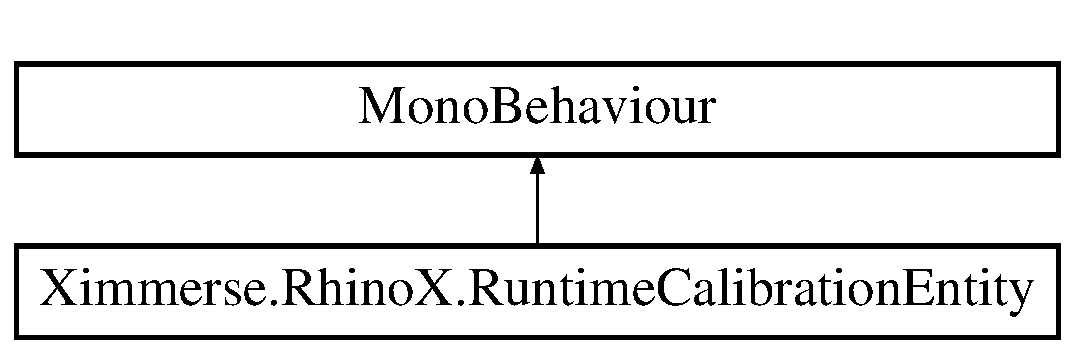
\includegraphics[height=2.000000cm]{class_ximmerse_1_1_rhino_x_1_1_runtime_calibration_entity}
\end{center}
\end{figure}
\subsection*{Public Member Functions}
\begin{DoxyCompactItemize}
\item 
\mbox{\Hypertarget{class_ximmerse_1_1_rhino_x_1_1_runtime_calibration_entity_a0dc5dfe6c0af4c0f8c079f1542e9fda6}\label{class_ximmerse_1_1_rhino_x_1_1_runtime_calibration_entity_a0dc5dfe6c0af4c0f8c079f1542e9fda6}} 
void {\bfseries Update\+Tracked\+Info} ()
\item 
float \mbox{\hyperlink{class_ximmerse_1_1_rhino_x_1_1_runtime_calibration_entity_a788798ab8698e05b46da74e84ebfbf14}{Update\+Calibration}} (\mbox{\hyperlink{class_ximmerse_1_1_rhino_x_1_1_runtime_calibration_entity}{Runtime\+Calibration\+Entity}} other)
\begin{DoxyCompactList}\small\item\em Updates the calibration. 更新对另一个已经标定的对象的标定数据. 要求 other 在调用此方法的时候可见。 返回一个 代表标定完成度的 normalized 的值。 \end{DoxyCompactList}\item 
byte \mbox{[}$\,$\mbox{]} \mbox{\hyperlink{class_ximmerse_1_1_rhino_x_1_1_runtime_calibration_entity_a5d385358e0eba30a11f5ac28c93f495c}{Serialize\+To\+Bytes}} ()
\begin{DoxyCompactList}\small\item\em Serialize the data of this entity to byte\mbox{[}\mbox{]} \end{DoxyCompactList}\end{DoxyCompactItemize}
\subsection*{Properties}
\begin{DoxyCompactItemize}
\item 
bool \mbox{\hyperlink{class_ximmerse_1_1_rhino_x_1_1_runtime_calibration_entity_a4089f89a884f71bd451b27d38ab978d0}{Is\+Calibrated}}\hspace{0.3cm}{\ttfamily  \mbox{[}get, set\mbox{]}}
\begin{DoxyCompactList}\small\item\em Gets or sets a value indicating whether this T\+:\+Runtime\+Calibration\+Entry is calibrated. \end{DoxyCompactList}\item 
\mbox{\Hypertarget{class_ximmerse_1_1_rhino_x_1_1_runtime_calibration_entity_af2d6869b466b8f5f0ead7eb434b95402}\label{class_ximmerse_1_1_rhino_x_1_1_runtime_calibration_entity_af2d6869b466b8f5f0ead7eb434b95402}} 
int {\bfseries Trackable\+ID}\hspace{0.3cm}{\ttfamily  \mbox{[}get\mbox{]}}
\item 
bool \mbox{\hyperlink{class_ximmerse_1_1_rhino_x_1_1_runtime_calibration_entity_ad9cfbd99981ebb2a69e1c5e8d6f5c92d}{Is\+Tracked}}\hspace{0.3cm}{\ttfamily  \mbox{[}get\mbox{]}}
\begin{DoxyCompactList}\small\item\em Gets a value indicating whether this T\+:\+Runtime\+Calibration\+Entry is tracked. \end{DoxyCompactList}\item 
\mbox{\Hypertarget{class_ximmerse_1_1_rhino_x_1_1_runtime_calibration_entity_a67a1202425a0a0bbe3c87539fb3117a3}\label{class_ximmerse_1_1_rhino_x_1_1_runtime_calibration_entity_a67a1202425a0a0bbe3c87539fb3117a3}} 
Vector3 {\bfseries Tracked\+Position}\hspace{0.3cm}{\ttfamily  \mbox{[}get\mbox{]}}
\item 
\mbox{\Hypertarget{class_ximmerse_1_1_rhino_x_1_1_runtime_calibration_entity_ab7958796c66a525f239f487e83067204}\label{class_ximmerse_1_1_rhino_x_1_1_runtime_calibration_entity_ab7958796c66a525f239f487e83067204}} 
Vector3 {\bfseries World\+Position}\hspace{0.3cm}{\ttfamily  \mbox{[}get\mbox{]}}
\item 
\mbox{\Hypertarget{class_ximmerse_1_1_rhino_x_1_1_runtime_calibration_entity_a59600142d6877b258221cfe5bb30ac3a}\label{class_ximmerse_1_1_rhino_x_1_1_runtime_calibration_entity_a59600142d6877b258221cfe5bb30ac3a}} 
Quaternion {\bfseries Tracked\+Rotation}\hspace{0.3cm}{\ttfamily  \mbox{[}get\mbox{]}}
\item 
\mbox{\Hypertarget{class_ximmerse_1_1_rhino_x_1_1_runtime_calibration_entity_a2b3850e48467f3c67eab5652cbfbc7ee}\label{class_ximmerse_1_1_rhino_x_1_1_runtime_calibration_entity_a2b3850e48467f3c67eab5652cbfbc7ee}} 
Quaternion {\bfseries World\+Rotation}\hspace{0.3cm}{\ttfamily  \mbox{[}get\mbox{]}}
\end{DoxyCompactItemize}
\subsection*{Events}
\begin{DoxyCompactItemize}
\item 
\mbox{\Hypertarget{class_ximmerse_1_1_rhino_x_1_1_runtime_calibration_entity_ab71d9cd08f0f16ad6e07e21d774ee8a0}\label{class_ximmerse_1_1_rhino_x_1_1_runtime_calibration_entity_ab71d9cd08f0f16ad6e07e21d774ee8a0}} 
System.\+Action$<$ \mbox{\hyperlink{class_ximmerse_1_1_rhino_x_1_1_runtime_calibration_entity}{Runtime\+Calibration\+Entity}} $>$ {\bfseries On\+Calibrated}
\end{DoxyCompactItemize}


\subsection{Detailed Description}
Runtime calibration entry. 



\subsection{Member Function Documentation}
\mbox{\Hypertarget{class_ximmerse_1_1_rhino_x_1_1_runtime_calibration_entity_a5d385358e0eba30a11f5ac28c93f495c}\label{class_ximmerse_1_1_rhino_x_1_1_runtime_calibration_entity_a5d385358e0eba30a11f5ac28c93f495c}} 
\index{Ximmerse\+::\+Rhino\+X\+::\+Runtime\+Calibration\+Entity@{Ximmerse\+::\+Rhino\+X\+::\+Runtime\+Calibration\+Entity}!Serialize\+To\+Bytes@{Serialize\+To\+Bytes}}
\index{Serialize\+To\+Bytes@{Serialize\+To\+Bytes}!Ximmerse\+::\+Rhino\+X\+::\+Runtime\+Calibration\+Entity@{Ximmerse\+::\+Rhino\+X\+::\+Runtime\+Calibration\+Entity}}
\subsubsection{\texorpdfstring{Serialize\+To\+Bytes()}{SerializeToBytes()}}
{\footnotesize\ttfamily byte \mbox{[}$\,$\mbox{]} Ximmerse.\+Rhino\+X.\+Runtime\+Calibration\+Entity.\+Serialize\+To\+Bytes (\begin{DoxyParamCaption}{ }\end{DoxyParamCaption})\hspace{0.3cm}{\ttfamily [inline]}}



Serialize the data of this entity to byte\mbox{[}\mbox{]} 

\begin{DoxyReturn}{Returns}
The to bytes.
\end{DoxyReturn}
\mbox{\Hypertarget{class_ximmerse_1_1_rhino_x_1_1_runtime_calibration_entity_a788798ab8698e05b46da74e84ebfbf14}\label{class_ximmerse_1_1_rhino_x_1_1_runtime_calibration_entity_a788798ab8698e05b46da74e84ebfbf14}} 
\index{Ximmerse\+::\+Rhino\+X\+::\+Runtime\+Calibration\+Entity@{Ximmerse\+::\+Rhino\+X\+::\+Runtime\+Calibration\+Entity}!Update\+Calibration@{Update\+Calibration}}
\index{Update\+Calibration@{Update\+Calibration}!Ximmerse\+::\+Rhino\+X\+::\+Runtime\+Calibration\+Entity@{Ximmerse\+::\+Rhino\+X\+::\+Runtime\+Calibration\+Entity}}
\subsubsection{\texorpdfstring{Update\+Calibration()}{UpdateCalibration()}}
{\footnotesize\ttfamily float Ximmerse.\+Rhino\+X.\+Runtime\+Calibration\+Entity.\+Update\+Calibration (\begin{DoxyParamCaption}\item[{\mbox{\hyperlink{class_ximmerse_1_1_rhino_x_1_1_runtime_calibration_entity}{Runtime\+Calibration\+Entity}}}]{other }\end{DoxyParamCaption})\hspace{0.3cm}{\ttfamily [inline]}}



Updates the calibration. 更新对另一个已经标定的对象的标定数据. 要求 other 在调用此方法的时候可见。 返回一个 代表标定完成度的 normalized 的值。 


\begin{DoxyParams}{Parameters}
{\em other} & Other.\\
\hline
\end{DoxyParams}


\subsection{Property Documentation}
\mbox{\Hypertarget{class_ximmerse_1_1_rhino_x_1_1_runtime_calibration_entity_a4089f89a884f71bd451b27d38ab978d0}\label{class_ximmerse_1_1_rhino_x_1_1_runtime_calibration_entity_a4089f89a884f71bd451b27d38ab978d0}} 
\index{Ximmerse\+::\+Rhino\+X\+::\+Runtime\+Calibration\+Entity@{Ximmerse\+::\+Rhino\+X\+::\+Runtime\+Calibration\+Entity}!Is\+Calibrated@{Is\+Calibrated}}
\index{Is\+Calibrated@{Is\+Calibrated}!Ximmerse\+::\+Rhino\+X\+::\+Runtime\+Calibration\+Entity@{Ximmerse\+::\+Rhino\+X\+::\+Runtime\+Calibration\+Entity}}
\subsubsection{\texorpdfstring{Is\+Calibrated}{IsCalibrated}}
{\footnotesize\ttfamily bool Ximmerse.\+Rhino\+X.\+Runtime\+Calibration\+Entity.\+Is\+Calibrated\hspace{0.3cm}{\ttfamily [get]}, {\ttfamily [set]}}



Gets or sets a value indicating whether this T\+:\+Runtime\+Calibration\+Entry is calibrated. 

{\ttfamily true} if is calibrated; otherwise, {\ttfamily false}.\mbox{\Hypertarget{class_ximmerse_1_1_rhino_x_1_1_runtime_calibration_entity_ad9cfbd99981ebb2a69e1c5e8d6f5c92d}\label{class_ximmerse_1_1_rhino_x_1_1_runtime_calibration_entity_ad9cfbd99981ebb2a69e1c5e8d6f5c92d}} 
\index{Ximmerse\+::\+Rhino\+X\+::\+Runtime\+Calibration\+Entity@{Ximmerse\+::\+Rhino\+X\+::\+Runtime\+Calibration\+Entity}!Is\+Tracked@{Is\+Tracked}}
\index{Is\+Tracked@{Is\+Tracked}!Ximmerse\+::\+Rhino\+X\+::\+Runtime\+Calibration\+Entity@{Ximmerse\+::\+Rhino\+X\+::\+Runtime\+Calibration\+Entity}}
\subsubsection{\texorpdfstring{Is\+Tracked}{IsTracked}}
{\footnotesize\ttfamily bool Ximmerse.\+Rhino\+X.\+Runtime\+Calibration\+Entity.\+Is\+Tracked\hspace{0.3cm}{\ttfamily [get]}}



Gets a value indicating whether this T\+:\+Runtime\+Calibration\+Entry is tracked. 

{\ttfamily true} if is tracked; otherwise, {\ttfamily false}.

The documentation for this class was generated from the following file\+:\begin{DoxyCompactItemize}
\item 
Calibration/Runtime\+Calibration\+Entity.\+cs\end{DoxyCompactItemize}

\hypertarget{class_ximmerse_1_1_rhino_x_1_1_runtime_calibration_manager}{}\section{Ximmerse.\+Rhino\+X.\+Runtime\+Calibration\+Manager Class Reference}
\label{class_ximmerse_1_1_rhino_x_1_1_runtime_calibration_manager}\index{Ximmerse.\+Rhino\+X.\+Runtime\+Calibration\+Manager@{Ximmerse.\+Rhino\+X.\+Runtime\+Calibration\+Manager}}


Runtime calibration manager.  


Inheritance diagram for Ximmerse.\+Rhino\+X.\+Runtime\+Calibration\+Manager\+:\begin{figure}[H]
\begin{center}
\leavevmode
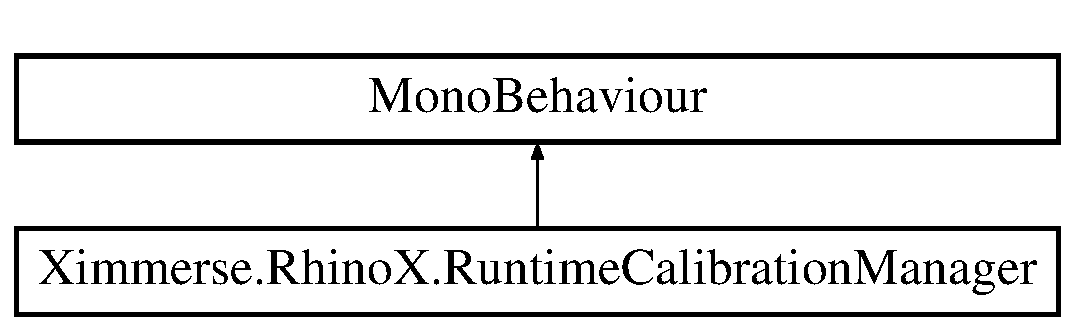
\includegraphics[height=2.000000cm]{class_ximmerse_1_1_rhino_x_1_1_runtime_calibration_manager}
\end{center}
\end{figure}
\subsection*{Public Member Functions}
\begin{DoxyCompactItemize}
\item 
void \mbox{\hyperlink{class_ximmerse_1_1_rhino_x_1_1_runtime_calibration_manager_a2eed7edd69a12c8ff0d3f8b4feb60f49}{Serialize\+Calibration\+Data}} ()
\begin{DoxyCompactList}\small\item\em Serializes the calibration data to /sdcard \end{DoxyCompactList}\end{DoxyCompactItemize}
\subsection*{Public Attributes}
\begin{DoxyCompactItemize}
\item 
List$<$ \mbox{\hyperlink{class_ximmerse_1_1_rhino_x_1_1_runtime_calibration_entity}{Runtime\+Calibration\+Entity}} $>$ \mbox{\hyperlink{class_ximmerse_1_1_rhino_x_1_1_runtime_calibration_manager_abf1b09b36bf1e6bccca57a451a263376}{Entities}}
\begin{DoxyCompactList}\small\item\em The trackable entries for calibration. \end{DoxyCompactList}\item 
\mbox{\Hypertarget{class_ximmerse_1_1_rhino_x_1_1_runtime_calibration_manager_abad22a1c28c38677a99cf817f4612595}\label{class_ximmerse_1_1_rhino_x_1_1_runtime_calibration_manager_abad22a1c28c38677a99cf817f4612595}} 
bool {\bfseries Auto\+Calibrated} = true
\end{DoxyCompactItemize}
\subsection*{Properties}
\begin{DoxyCompactItemize}
\item 
\mbox{\hyperlink{class_ximmerse_1_1_rhino_x_1_1_runtime_calibration_entity}{Runtime\+Calibration\+Entity}} \mbox{\hyperlink{class_ximmerse_1_1_rhino_x_1_1_runtime_calibration_manager_a1202f2b01cb1c6e6ee7f332ee0ad9e97}{Center\+Entry}}\hspace{0.3cm}{\ttfamily  \mbox{[}get, set\mbox{]}}
\begin{DoxyCompactList}\small\item\em Gets or sets the center entry. \end{DoxyCompactList}\end{DoxyCompactItemize}


\subsection{Detailed Description}
Runtime calibration manager. 



\subsection{Member Function Documentation}
\mbox{\Hypertarget{class_ximmerse_1_1_rhino_x_1_1_runtime_calibration_manager_a2eed7edd69a12c8ff0d3f8b4feb60f49}\label{class_ximmerse_1_1_rhino_x_1_1_runtime_calibration_manager_a2eed7edd69a12c8ff0d3f8b4feb60f49}} 
\index{Ximmerse\+::\+Rhino\+X\+::\+Runtime\+Calibration\+Manager@{Ximmerse\+::\+Rhino\+X\+::\+Runtime\+Calibration\+Manager}!Serialize\+Calibration\+Data@{Serialize\+Calibration\+Data}}
\index{Serialize\+Calibration\+Data@{Serialize\+Calibration\+Data}!Ximmerse\+::\+Rhino\+X\+::\+Runtime\+Calibration\+Manager@{Ximmerse\+::\+Rhino\+X\+::\+Runtime\+Calibration\+Manager}}
\subsubsection{\texorpdfstring{Serialize\+Calibration\+Data()}{SerializeCalibrationData()}}
{\footnotesize\ttfamily void Ximmerse.\+Rhino\+X.\+Runtime\+Calibration\+Manager.\+Serialize\+Calibration\+Data (\begin{DoxyParamCaption}{ }\end{DoxyParamCaption})}



Serializes the calibration data to /sdcard 



\subsection{Member Data Documentation}
\mbox{\Hypertarget{class_ximmerse_1_1_rhino_x_1_1_runtime_calibration_manager_abf1b09b36bf1e6bccca57a451a263376}\label{class_ximmerse_1_1_rhino_x_1_1_runtime_calibration_manager_abf1b09b36bf1e6bccca57a451a263376}} 
\index{Ximmerse\+::\+Rhino\+X\+::\+Runtime\+Calibration\+Manager@{Ximmerse\+::\+Rhino\+X\+::\+Runtime\+Calibration\+Manager}!Entities@{Entities}}
\index{Entities@{Entities}!Ximmerse\+::\+Rhino\+X\+::\+Runtime\+Calibration\+Manager@{Ximmerse\+::\+Rhino\+X\+::\+Runtime\+Calibration\+Manager}}
\subsubsection{\texorpdfstring{Entities}{Entities}}
{\footnotesize\ttfamily List$<$\mbox{\hyperlink{class_ximmerse_1_1_rhino_x_1_1_runtime_calibration_entity}{Runtime\+Calibration\+Entity}}$>$ Ximmerse.\+Rhino\+X.\+Runtime\+Calibration\+Manager.\+Entities}



The trackable entries for calibration. 



\subsection{Property Documentation}
\mbox{\Hypertarget{class_ximmerse_1_1_rhino_x_1_1_runtime_calibration_manager_a1202f2b01cb1c6e6ee7f332ee0ad9e97}\label{class_ximmerse_1_1_rhino_x_1_1_runtime_calibration_manager_a1202f2b01cb1c6e6ee7f332ee0ad9e97}} 
\index{Ximmerse\+::\+Rhino\+X\+::\+Runtime\+Calibration\+Manager@{Ximmerse\+::\+Rhino\+X\+::\+Runtime\+Calibration\+Manager}!Center\+Entry@{Center\+Entry}}
\index{Center\+Entry@{Center\+Entry}!Ximmerse\+::\+Rhino\+X\+::\+Runtime\+Calibration\+Manager@{Ximmerse\+::\+Rhino\+X\+::\+Runtime\+Calibration\+Manager}}
\subsubsection{\texorpdfstring{Center\+Entry}{CenterEntry}}
{\footnotesize\ttfamily \mbox{\hyperlink{class_ximmerse_1_1_rhino_x_1_1_runtime_calibration_entity}{Runtime\+Calibration\+Entity}} Ximmerse.\+Rhino\+X.\+Runtime\+Calibration\+Manager.\+Center\+Entry\hspace{0.3cm}{\ttfamily [get]}, {\ttfamily [set]}}



Gets or sets the center entry. 

The center.

The documentation for this class was generated from the following file\+:\begin{DoxyCompactItemize}
\item 
H\+L\+A\+P\+I/\+Public/\+Calibration/Runtime\+Calibration\+Manager.\+cs\end{DoxyCompactItemize}

\hypertarget{class_ximmerse_1_1_rhino_x_1_1_r_x_controller}{}\section{Ximmerse.\+Rhino\+X.\+R\+X\+Controller Class Reference}
\label{class_ximmerse_1_1_rhino_x_1_1_r_x_controller}\index{Ximmerse.\+Rhino\+X.\+R\+X\+Controller@{Ximmerse.\+Rhino\+X.\+R\+X\+Controller}}


High level S\+DK script for developers to access controller data and event, e.\+g. buttons, gyroscopes, finger point over touch-\/pad.  


Inheritance diagram for Ximmerse.\+Rhino\+X.\+R\+X\+Controller\+:\begin{figure}[H]
\begin{center}
\leavevmode
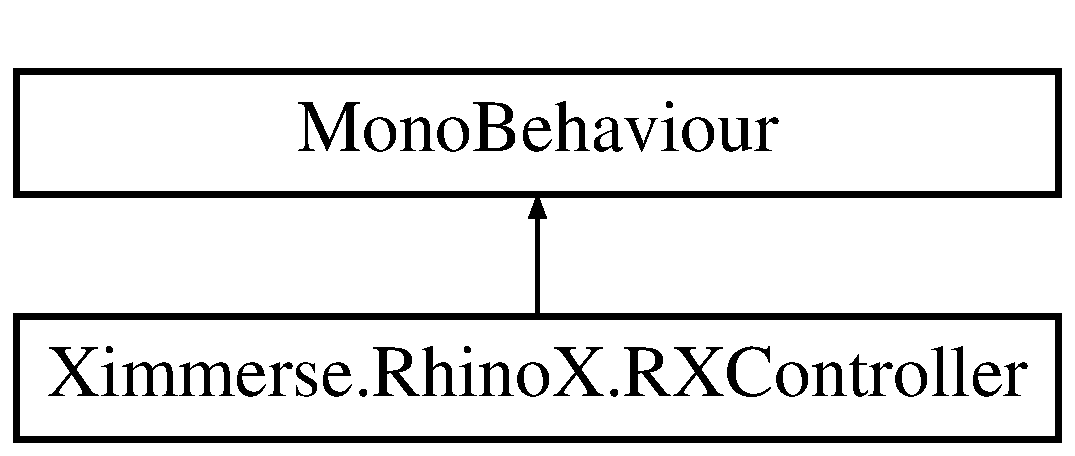
\includegraphics[height=2.000000cm]{class_ximmerse_1_1_rhino_x_1_1_r_x_controller}
\end{center}
\end{figure}
\subsection*{Classes}
\begin{DoxyCompactItemize}
\item 
class \mbox{\hyperlink{class_ximmerse_1_1_rhino_x_1_1_r_x_controller_1_1_controller_button_event}{Controller\+Button\+Event}}
\end{DoxyCompactItemize}
\subsection*{Public Member Functions}
\begin{DoxyCompactItemize}
\item 
bool \mbox{\hyperlink{class_ximmerse_1_1_rhino_x_1_1_r_x_controller_a89fb2bd2521d43205645fb6b205ddbcf}{Is\+Tap}} (\mbox{\hyperlink{namespace_ximmerse_1_1_rhino_x_a99f73f11bba9d4b424daba6c5a5abc0b}{Controller\+Button\+Code}} button)
\begin{DoxyCompactList}\small\item\em Is user taping the specific button ? \end{DoxyCompactList}\item 
bool \mbox{\hyperlink{class_ximmerse_1_1_rhino_x_1_1_r_x_controller_aa9d23fdcda8d7e24e342c26e5b8d6b27}{Is\+Press}} (\mbox{\hyperlink{namespace_ximmerse_1_1_rhino_x_a99f73f11bba9d4b424daba6c5a5abc0b}{Controller\+Button\+Code}} button)
\begin{DoxyCompactList}\small\item\em Is user current holding the button down ? \end{DoxyCompactList}\end{DoxyCompactItemize}
\subsection*{Public Attributes}
\begin{DoxyCompactItemize}
\item 
\mbox{\Hypertarget{class_ximmerse_1_1_rhino_x_1_1_r_x_controller_a0a0b1610bfceaf7fa12aa7c77d86e79a}\label{class_ximmerse_1_1_rhino_x_1_1_r_x_controller_a0a0b1610bfceaf7fa12aa7c77d86e79a}} 
\mbox{\hyperlink{class_ximmerse_1_1_rhino_x_1_1_r_x_controller_1_1_controller_button_event}{Controller\+Button\+Event}} {\bfseries On\+Key\+Down} = new \mbox{\hyperlink{class_ximmerse_1_1_rhino_x_1_1_r_x_controller_1_1_controller_button_event}{Controller\+Button\+Event}}()
\item 
\mbox{\Hypertarget{class_ximmerse_1_1_rhino_x_1_1_r_x_controller_a07521aeb769bd91e46f43844c2191c6d}\label{class_ximmerse_1_1_rhino_x_1_1_r_x_controller_a07521aeb769bd91e46f43844c2191c6d}} 
\mbox{\hyperlink{class_ximmerse_1_1_rhino_x_1_1_r_x_controller_1_1_controller_button_event}{Controller\+Button\+Event}} {\bfseries On\+Tap} = new \mbox{\hyperlink{class_ximmerse_1_1_rhino_x_1_1_r_x_controller_1_1_controller_button_event}{Controller\+Button\+Event}}()
\item 
\mbox{\Hypertarget{class_ximmerse_1_1_rhino_x_1_1_r_x_controller_afc517f2529c9294a037562763c0088ef}\label{class_ximmerse_1_1_rhino_x_1_1_r_x_controller_afc517f2529c9294a037562763c0088ef}} 
\mbox{\hyperlink{class_ximmerse_1_1_rhino_x_1_1_r_x_controller_1_1_controller_button_event}{Controller\+Button\+Event}} {\bfseries On\+Key\+Up} = new \mbox{\hyperlink{class_ximmerse_1_1_rhino_x_1_1_r_x_controller_1_1_controller_button_event}{Controller\+Button\+Event}}()
\item 
\mbox{\Hypertarget{class_ximmerse_1_1_rhino_x_1_1_r_x_controller_a2857dbbb67e691e9c441af16e622a77b}\label{class_ximmerse_1_1_rhino_x_1_1_r_x_controller_a2857dbbb67e691e9c441af16e622a77b}} 
\mbox{\hyperlink{struct_ximmerse_1_1_rhino_x_1_1_controller_gyroscope}{Controller\+Gyroscope}} {\bfseries gyroscope} = new \mbox{\hyperlink{struct_ximmerse_1_1_rhino_x_1_1_controller_gyroscope}{Controller\+Gyroscope}}()
\item 
\mbox{\Hypertarget{class_ximmerse_1_1_rhino_x_1_1_r_x_controller_af0f42078b3ae1b984bc9cba98e0571e5}\label{class_ximmerse_1_1_rhino_x_1_1_r_x_controller_af0f42078b3ae1b984bc9cba98e0571e5}} 
bool {\bfseries Debug\+Log}
\end{DoxyCompactItemize}
\subsection*{Properties}
\begin{DoxyCompactItemize}
\item 
\mbox{\hyperlink{namespace_ximmerse_1_1_rhino_x_a78c4d1657dc299dc9f91fad0ef234666}{Controller\+Index}} \mbox{\hyperlink{class_ximmerse_1_1_rhino_x_1_1_r_x_controller_a74749f7219b9eca23f4540de4c98fc48}{Index}}\hspace{0.3cm}{\ttfamily  \mbox{[}get, set\mbox{]}}
\begin{DoxyCompactList}\small\item\em Gets or sets the index the controller that this instance pairs to. \end{DoxyCompactList}\item 
\mbox{\hyperlink{class_ximmerse_1_1_rhino_x_1_1_r_x_raycaster}{R\+X\+Raycaster}} \mbox{\hyperlink{class_ximmerse_1_1_rhino_x_1_1_r_x_controller_a777648a528c40d7221682ba898562c95}{raycaster}}\hspace{0.3cm}{\ttfamily  \mbox{[}get, set\mbox{]}}
\begin{DoxyCompactList}\small\item\em Gets or sets the raycaster that this controller bounds to. \end{DoxyCompactList}\item 
bool \mbox{\hyperlink{class_ximmerse_1_1_rhino_x_1_1_r_x_controller_ac7f62ba234dae32195cd95530a8e2879}{Has\+Touch\+Pad\+Point}}\hspace{0.3cm}{\ttfamily  \mbox{[}get\mbox{]}}
\begin{DoxyCompactList}\small\item\em When using \mbox{\hyperlink{namespace_ximmerse}{Ximmerse}} flip controller, this properties indicates if player has finger down on touch pad. \end{DoxyCompactList}\item 
Vector2 \mbox{\hyperlink{class_ximmerse_1_1_rhino_x_1_1_r_x_controller_ae9a2c7113e7cdc7d802b500d628a2c1c}{Touch\+Pad\+Point}}\hspace{0.3cm}{\ttfamily  \mbox{[}get\mbox{]}}
\begin{DoxyCompactList}\small\item\em Gets the touch pad pointer value, when Has\+Touch\+Pad\+Point = true. \end{DoxyCompactList}\end{DoxyCompactItemize}


\subsection{Detailed Description}
High level S\+DK script for developers to access controller data and event, e.\+g. buttons, gyroscopes, finger point over touch-\/pad. 



\subsection{Member Function Documentation}
\mbox{\Hypertarget{class_ximmerse_1_1_rhino_x_1_1_r_x_controller_aa9d23fdcda8d7e24e342c26e5b8d6b27}\label{class_ximmerse_1_1_rhino_x_1_1_r_x_controller_aa9d23fdcda8d7e24e342c26e5b8d6b27}} 
\index{Ximmerse\+::\+Rhino\+X\+::\+R\+X\+Controller@{Ximmerse\+::\+Rhino\+X\+::\+R\+X\+Controller}!Is\+Press@{Is\+Press}}
\index{Is\+Press@{Is\+Press}!Ximmerse\+::\+Rhino\+X\+::\+R\+X\+Controller@{Ximmerse\+::\+Rhino\+X\+::\+R\+X\+Controller}}
\subsubsection{\texorpdfstring{Is\+Press()}{IsPress()}}
{\footnotesize\ttfamily bool Ximmerse.\+Rhino\+X.\+R\+X\+Controller.\+Is\+Press (\begin{DoxyParamCaption}\item[{\mbox{\hyperlink{namespace_ximmerse_1_1_rhino_x_a99f73f11bba9d4b424daba6c5a5abc0b}{Controller\+Button\+Code}}}]{button }\end{DoxyParamCaption})\hspace{0.3cm}{\ttfamily [inline]}}



Is user current holding the button down ? 

\begin{DoxyReturn}{Returns}
{\ttfamily true}, if press was ised, {\ttfamily false} otherwise.
\end{DoxyReturn}

\begin{DoxyParams}{Parameters}
{\em button} & Button.\\
\hline
\end{DoxyParams}
\mbox{\Hypertarget{class_ximmerse_1_1_rhino_x_1_1_r_x_controller_a89fb2bd2521d43205645fb6b205ddbcf}\label{class_ximmerse_1_1_rhino_x_1_1_r_x_controller_a89fb2bd2521d43205645fb6b205ddbcf}} 
\index{Ximmerse\+::\+Rhino\+X\+::\+R\+X\+Controller@{Ximmerse\+::\+Rhino\+X\+::\+R\+X\+Controller}!Is\+Tap@{Is\+Tap}}
\index{Is\+Tap@{Is\+Tap}!Ximmerse\+::\+Rhino\+X\+::\+R\+X\+Controller@{Ximmerse\+::\+Rhino\+X\+::\+R\+X\+Controller}}
\subsubsection{\texorpdfstring{Is\+Tap()}{IsTap()}}
{\footnotesize\ttfamily bool Ximmerse.\+Rhino\+X.\+R\+X\+Controller.\+Is\+Tap (\begin{DoxyParamCaption}\item[{\mbox{\hyperlink{namespace_ximmerse_1_1_rhino_x_a99f73f11bba9d4b424daba6c5a5abc0b}{Controller\+Button\+Code}}}]{button }\end{DoxyParamCaption})\hspace{0.3cm}{\ttfamily [inline]}}



Is user taping the specific button ? 

\begin{DoxyReturn}{Returns}
{\ttfamily true}, if tap was ised, {\ttfamily false} otherwise.
\end{DoxyReturn}

\begin{DoxyParams}{Parameters}
{\em button} & Button.\\
\hline
\end{DoxyParams}


\subsection{Property Documentation}
\mbox{\Hypertarget{class_ximmerse_1_1_rhino_x_1_1_r_x_controller_ac7f62ba234dae32195cd95530a8e2879}\label{class_ximmerse_1_1_rhino_x_1_1_r_x_controller_ac7f62ba234dae32195cd95530a8e2879}} 
\index{Ximmerse\+::\+Rhino\+X\+::\+R\+X\+Controller@{Ximmerse\+::\+Rhino\+X\+::\+R\+X\+Controller}!Has\+Touch\+Pad\+Point@{Has\+Touch\+Pad\+Point}}
\index{Has\+Touch\+Pad\+Point@{Has\+Touch\+Pad\+Point}!Ximmerse\+::\+Rhino\+X\+::\+R\+X\+Controller@{Ximmerse\+::\+Rhino\+X\+::\+R\+X\+Controller}}
\subsubsection{\texorpdfstring{Has\+Touch\+Pad\+Point}{HasTouchPadPoint}}
{\footnotesize\ttfamily bool Ximmerse.\+Rhino\+X.\+R\+X\+Controller.\+Has\+Touch\+Pad\+Point\hspace{0.3cm}{\ttfamily [get]}}



When using \mbox{\hyperlink{namespace_ximmerse}{Ximmerse}} flip controller, this properties indicates if player has finger down on touch pad. 

{\ttfamily true} if has touch point; otherwise, {\ttfamily false}.\mbox{\Hypertarget{class_ximmerse_1_1_rhino_x_1_1_r_x_controller_a74749f7219b9eca23f4540de4c98fc48}\label{class_ximmerse_1_1_rhino_x_1_1_r_x_controller_a74749f7219b9eca23f4540de4c98fc48}} 
\index{Ximmerse\+::\+Rhino\+X\+::\+R\+X\+Controller@{Ximmerse\+::\+Rhino\+X\+::\+R\+X\+Controller}!Index@{Index}}
\index{Index@{Index}!Ximmerse\+::\+Rhino\+X\+::\+R\+X\+Controller@{Ximmerse\+::\+Rhino\+X\+::\+R\+X\+Controller}}
\subsubsection{\texorpdfstring{Index}{Index}}
{\footnotesize\ttfamily \mbox{\hyperlink{namespace_ximmerse_1_1_rhino_x_a78c4d1657dc299dc9f91fad0ef234666}{Controller\+Index}} Ximmerse.\+Rhino\+X.\+R\+X\+Controller.\+Index\hspace{0.3cm}{\ttfamily [get]}, {\ttfamily [set]}}



Gets or sets the index the controller that this instance pairs to. 

The index.\mbox{\Hypertarget{class_ximmerse_1_1_rhino_x_1_1_r_x_controller_a777648a528c40d7221682ba898562c95}\label{class_ximmerse_1_1_rhino_x_1_1_r_x_controller_a777648a528c40d7221682ba898562c95}} 
\index{Ximmerse\+::\+Rhino\+X\+::\+R\+X\+Controller@{Ximmerse\+::\+Rhino\+X\+::\+R\+X\+Controller}!raycaster@{raycaster}}
\index{raycaster@{raycaster}!Ximmerse\+::\+Rhino\+X\+::\+R\+X\+Controller@{Ximmerse\+::\+Rhino\+X\+::\+R\+X\+Controller}}
\subsubsection{\texorpdfstring{raycaster}{raycaster}}
{\footnotesize\ttfamily \mbox{\hyperlink{class_ximmerse_1_1_rhino_x_1_1_r_x_raycaster}{R\+X\+Raycaster}} Ximmerse.\+Rhino\+X.\+R\+X\+Controller.\+raycaster\hspace{0.3cm}{\ttfamily [get]}, {\ttfamily [set]}}



Gets or sets the raycaster that this controller bounds to. 

The raycaster.\mbox{\Hypertarget{class_ximmerse_1_1_rhino_x_1_1_r_x_controller_ae9a2c7113e7cdc7d802b500d628a2c1c}\label{class_ximmerse_1_1_rhino_x_1_1_r_x_controller_ae9a2c7113e7cdc7d802b500d628a2c1c}} 
\index{Ximmerse\+::\+Rhino\+X\+::\+R\+X\+Controller@{Ximmerse\+::\+Rhino\+X\+::\+R\+X\+Controller}!Touch\+Pad\+Point@{Touch\+Pad\+Point}}
\index{Touch\+Pad\+Point@{Touch\+Pad\+Point}!Ximmerse\+::\+Rhino\+X\+::\+R\+X\+Controller@{Ximmerse\+::\+Rhino\+X\+::\+R\+X\+Controller}}
\subsubsection{\texorpdfstring{Touch\+Pad\+Point}{TouchPadPoint}}
{\footnotesize\ttfamily Vector2 Ximmerse.\+Rhino\+X.\+R\+X\+Controller.\+Touch\+Pad\+Point\hspace{0.3cm}{\ttfamily [get]}}



Gets the touch pad pointer value, when Has\+Touch\+Pad\+Point = true. 

The touch pad point.

The documentation for this class was generated from the following file\+:\begin{DoxyCompactItemize}
\item 
Event\+System/R\+X\+Controller.\+cs\end{DoxyCompactItemize}

\hypertarget{class_ximmerse_1_1_rhino_x_1_1_r_x_event_system}{}\section{Ximmerse.\+Rhino\+X.\+R\+X\+Event\+System Class Reference}
\label{class_ximmerse_1_1_rhino_x_1_1_r_x_event_system}\index{Ximmerse.\+Rhino\+X.\+R\+X\+Event\+System@{Ximmerse.\+Rhino\+X.\+R\+X\+Event\+System}}


\mbox{\hyperlink{namespace_ximmerse_1_1_rhino_x}{RhinoX}} event system, should be singleton instance, driver class of \mbox{\hyperlink{namespace_ximmerse_1_1_rhino_x}{RhinoX}} input event system. Note\+: \mbox{\hyperlink{class_ximmerse_1_1_rhino_x_1_1_r_x_event_system}{R\+X\+Event\+System}} need to be the only event system, if your scene has Unity\textquotesingle{}s built in Event\+System instane, \mbox{\hyperlink{class_ximmerse_1_1_rhino_x_1_1_r_x_event_system}{R\+X\+Event\+System}} will remove it when starts.  


Inheritance diagram for Ximmerse.\+Rhino\+X.\+R\+X\+Event\+System\+:\begin{figure}[H]
\begin{center}
\leavevmode
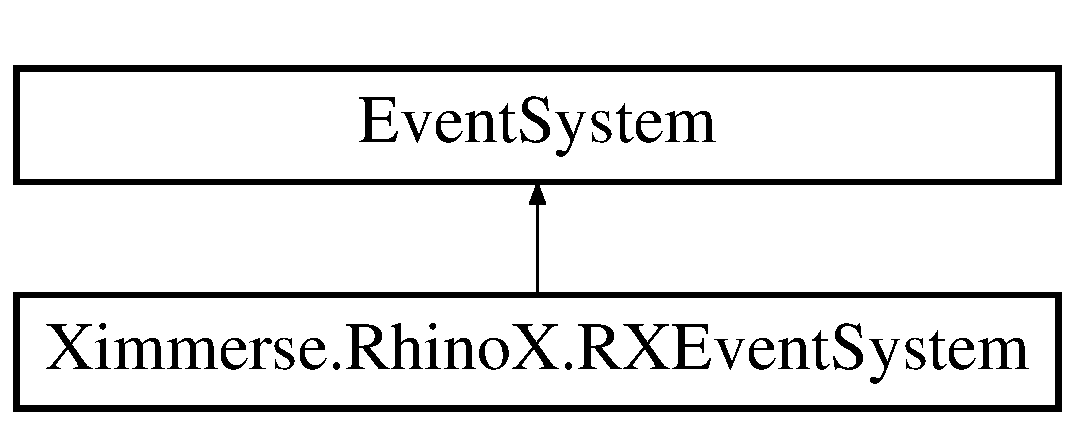
\includegraphics[height=2.000000cm]{class_ximmerse_1_1_rhino_x_1_1_r_x_event_system}
\end{center}
\end{figure}
\subsection*{Protected Member Functions}
\begin{DoxyCompactItemize}
\item 
\mbox{\Hypertarget{class_ximmerse_1_1_rhino_x_1_1_r_x_event_system_afff01ad9feb8e0a4257fbcaf5fe908d3}\label{class_ximmerse_1_1_rhino_x_1_1_r_x_event_system_afff01ad9feb8e0a4257fbcaf5fe908d3}} 
override void {\bfseries Awake} ()
\item 
\mbox{\Hypertarget{class_ximmerse_1_1_rhino_x_1_1_r_x_event_system_ad4eb777be634608e7cb3668e6773bad4}\label{class_ximmerse_1_1_rhino_x_1_1_r_x_event_system_ad4eb777be634608e7cb3668e6773bad4}} 
override void {\bfseries Update} ()
\item 
\mbox{\Hypertarget{class_ximmerse_1_1_rhino_x_1_1_r_x_event_system_a8d8a80f01e2361e2be206d6cc9d5a58f}\label{class_ximmerse_1_1_rhino_x_1_1_r_x_event_system_a8d8a80f01e2361e2be206d6cc9d5a58f}} 
override void {\bfseries On\+Application\+Focus} (bool has\+Focus)
\end{DoxyCompactItemize}


\subsection{Detailed Description}
\mbox{\hyperlink{namespace_ximmerse_1_1_rhino_x}{RhinoX}} event system, should be singleton instance, driver class of \mbox{\hyperlink{namespace_ximmerse_1_1_rhino_x}{RhinoX}} input event system. Note\+: \mbox{\hyperlink{class_ximmerse_1_1_rhino_x_1_1_r_x_event_system}{R\+X\+Event\+System}} need to be the only event system, if your scene has Unity\textquotesingle{}s built in Event\+System instane, \mbox{\hyperlink{class_ximmerse_1_1_rhino_x_1_1_r_x_event_system}{R\+X\+Event\+System}} will remove it when starts. 



The documentation for this class was generated from the following file\+:\begin{DoxyCompactItemize}
\item 
H\+L\+A\+P\+I/\+Public/\+Event\+System/R\+X\+Event\+System.\+cs\end{DoxyCompactItemize}

\hypertarget{class_ximmerse_1_1_rhino_x_1_1_r_x_input_module}{}\section{Ximmerse.\+Rhino\+X.\+R\+X\+Input\+Module Class Reference}
\label{class_ximmerse_1_1_rhino_x_1_1_r_x_input_module}\index{Ximmerse.\+Rhino\+X.\+R\+X\+Input\+Module@{Ximmerse.\+Rhino\+X.\+R\+X\+Input\+Module}}


\mbox{\hyperlink{namespace_ximmerse_1_1_rhino_x}{RhinoX}} controller module, public interface to ximmerse controller input event system.  


Inheritance diagram for Ximmerse.\+Rhino\+X.\+R\+X\+Input\+Module\+:\begin{figure}[H]
\begin{center}
\leavevmode
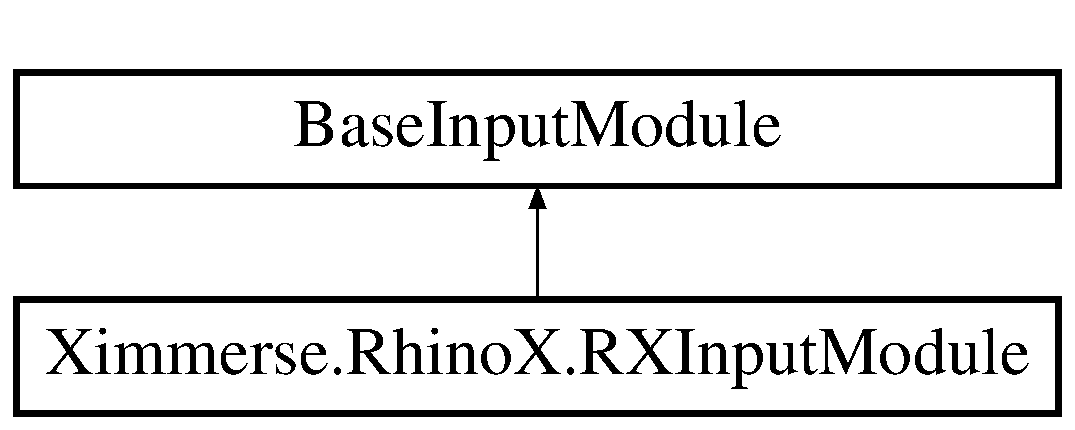
\includegraphics[height=2.000000cm]{class_ximmerse_1_1_rhino_x_1_1_r_x_input_module}
\end{center}
\end{figure}
\subsection*{Public Member Functions}
\begin{DoxyCompactItemize}
\item 
\mbox{\Hypertarget{class_ximmerse_1_1_rhino_x_1_1_r_x_input_module_a10c2e45a017d04fe95e8ae672ca99c41}\label{class_ximmerse_1_1_rhino_x_1_1_r_x_input_module_a10c2e45a017d04fe95e8ae672ca99c41}} 
override bool {\bfseries Should\+Activate\+Module} ()
\item 
\mbox{\Hypertarget{class_ximmerse_1_1_rhino_x_1_1_r_x_input_module_a246990c38b35231c5b32aae3b40a826f}\label{class_ximmerse_1_1_rhino_x_1_1_r_x_input_module_a246990c38b35231c5b32aae3b40a826f}} 
override bool {\bfseries Is\+Module\+Supported} ()
\item 
\mbox{\Hypertarget{class_ximmerse_1_1_rhino_x_1_1_r_x_input_module_a94c6f2a3ccff6bb93440417436bf6295}\label{class_ximmerse_1_1_rhino_x_1_1_r_x_input_module_a94c6f2a3ccff6bb93440417436bf6295}} 
override void {\bfseries Process} ()
\end{DoxyCompactItemize}
\subsection*{Protected Member Functions}
\begin{DoxyCompactItemize}
\item 
\mbox{\Hypertarget{class_ximmerse_1_1_rhino_x_1_1_r_x_input_module_a970861dbb52ca7f297afd42bbc2638bc}\label{class_ximmerse_1_1_rhino_x_1_1_r_x_input_module_a970861dbb52ca7f297afd42bbc2638bc}} 
override void {\bfseries Awake} ()
\end{DoxyCompactItemize}
\subsection*{Properties}
\begin{DoxyCompactItemize}
\item 
\mbox{\Hypertarget{class_ximmerse_1_1_rhino_x_1_1_r_x_input_module_a16ef45842c84483dcaa87c042459f7f2}\label{class_ximmerse_1_1_rhino_x_1_1_r_x_input_module_a16ef45842c84483dcaa87c042459f7f2}} 
static \mbox{\hyperlink{class_ximmerse_1_1_rhino_x_1_1_r_x_input_module}{R\+X\+Input\+Module}} {\bfseries Instance}\hspace{0.3cm}{\ttfamily  \mbox{[}get\mbox{]}}
\item 
\mbox{\hyperlink{namespace_ximmerse_1_1_rhino_x_a99f73f11bba9d4b424daba6c5a5abc0b}{Controller\+Button\+Code}} \mbox{\hyperlink{class_ximmerse_1_1_rhino_x_1_1_r_x_input_module_a0b32ffc354f00d3e4db96ad7ac43bb35}{Pointer\+Button}}\hspace{0.3cm}{\ttfamily  \mbox{[}get, set\mbox{]}}
\begin{DoxyCompactList}\small\item\em Gets or sets the pointer button. This is the button to trigger pointer event, such as Pointer\+Click, Drag. \end{DoxyCompactList}\end{DoxyCompactItemize}


\subsection{Detailed Description}
\mbox{\hyperlink{namespace_ximmerse_1_1_rhino_x}{RhinoX}} controller module, public interface to ximmerse controller input event system. 



\subsection{Property Documentation}
\mbox{\Hypertarget{class_ximmerse_1_1_rhino_x_1_1_r_x_input_module_a0b32ffc354f00d3e4db96ad7ac43bb35}\label{class_ximmerse_1_1_rhino_x_1_1_r_x_input_module_a0b32ffc354f00d3e4db96ad7ac43bb35}} 
\index{Ximmerse\+::\+Rhino\+X\+::\+R\+X\+Input\+Module@{Ximmerse\+::\+Rhino\+X\+::\+R\+X\+Input\+Module}!Pointer\+Button@{Pointer\+Button}}
\index{Pointer\+Button@{Pointer\+Button}!Ximmerse\+::\+Rhino\+X\+::\+R\+X\+Input\+Module@{Ximmerse\+::\+Rhino\+X\+::\+R\+X\+Input\+Module}}
\subsubsection{\texorpdfstring{Pointer\+Button}{PointerButton}}
{\footnotesize\ttfamily \mbox{\hyperlink{namespace_ximmerse_1_1_rhino_x_a99f73f11bba9d4b424daba6c5a5abc0b}{Controller\+Button\+Code}} Ximmerse.\+Rhino\+X.\+R\+X\+Input\+Module.\+Pointer\+Button\hspace{0.3cm}{\ttfamily [get]}, {\ttfamily [set]}}



Gets or sets the pointer button. This is the button to trigger pointer event, such as Pointer\+Click, Drag. 

The pointer button.

The documentation for this class was generated from the following file\+:\begin{DoxyCompactItemize}
\item 
H\+L\+A\+P\+I/\+Public/\+Event\+System/R\+X\+Input\+Module.\+cs\end{DoxyCompactItemize}

\hypertarget{class_ximmerse_1_1_rhino_x_1_1_r_x_raycaster}{}\section{Ximmerse.\+Rhino\+X.\+R\+X\+Raycaster Class Reference}
\label{class_ximmerse_1_1_rhino_x_1_1_r_x_raycaster}\index{Ximmerse.\+Rhino\+X.\+R\+X\+Raycaster@{Ximmerse.\+Rhino\+X.\+R\+X\+Raycaster}}


Rhino-\/X raycaster.  


Inheritance diagram for Ximmerse.\+Rhino\+X.\+R\+X\+Raycaster\+:\begin{figure}[H]
\begin{center}
\leavevmode
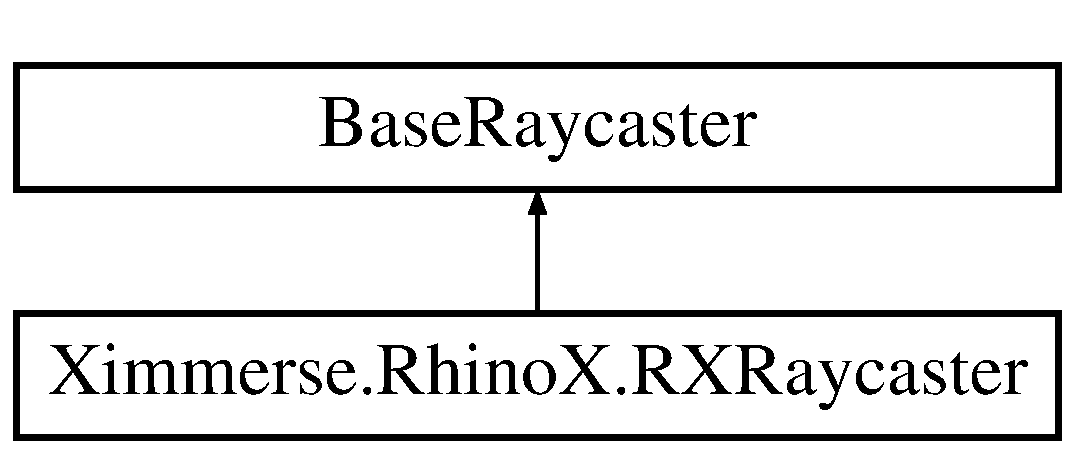
\includegraphics[height=2.000000cm]{class_ximmerse_1_1_rhino_x_1_1_r_x_raycaster}
\end{center}
\end{figure}
\subsection*{Public Member Functions}
\begin{DoxyCompactItemize}
\item 
\mbox{\Hypertarget{class_ximmerse_1_1_rhino_x_1_1_r_x_raycaster_aeb344747b5d79275be7dbfe65f3c123d}\label{class_ximmerse_1_1_rhino_x_1_1_r_x_raycaster_aeb344747b5d79275be7dbfe65f3c123d}} 
override void {\bfseries Raycast} (Pointer\+Event\+Data event\+Data, List$<$ Raycast\+Result $>$ result\+Append\+List)
\end{DoxyCompactItemize}
\subsection*{Protected Member Functions}
\begin{DoxyCompactItemize}
\item 
\mbox{\Hypertarget{class_ximmerse_1_1_rhino_x_1_1_r_x_raycaster_a54c7a5659ffdecb608cf3dd1b27ded40}\label{class_ximmerse_1_1_rhino_x_1_1_r_x_raycaster_a54c7a5659ffdecb608cf3dd1b27ded40}} 
override void {\bfseries On\+Enable} ()
\item 
\mbox{\Hypertarget{class_ximmerse_1_1_rhino_x_1_1_r_x_raycaster_a9f7c917a1aab68fff8421d7c50f2760d}\label{class_ximmerse_1_1_rhino_x_1_1_r_x_raycaster_a9f7c917a1aab68fff8421d7c50f2760d}} 
override void {\bfseries On\+Disable} ()
\end{DoxyCompactItemize}
\subsection*{Properties}
\begin{DoxyCompactItemize}
\item 
Layer\+Mask \mbox{\hyperlink{class_ximmerse_1_1_rhino_x_1_1_r_x_raycaster_a86b39123e4c2487a2906369278e075f8}{Culling\+Mask}}\hspace{0.3cm}{\ttfamily  \mbox{[}get, set\mbox{]}}
\begin{DoxyCompactList}\small\item\em Culling mask of interaction object. By default, interaction with Ui object. \end{DoxyCompactList}\item 
float \mbox{\hyperlink{class_ximmerse_1_1_rhino_x_1_1_r_x_raycaster_a122146e73455860e6aaf030211fe948c}{Raycast\+Distance}}\hspace{0.3cm}{\ttfamily  \mbox{[}get, set\mbox{]}}
\begin{DoxyCompactList}\small\item\em Raycast distance \end{DoxyCompactList}\item 
\mbox{\Hypertarget{class_ximmerse_1_1_rhino_x_1_1_r_x_raycaster_a86af80ce816c32ad5fb680c6a67716a1}\label{class_ximmerse_1_1_rhino_x_1_1_r_x_raycaster_a86af80ce816c32ad5fb680c6a67716a1}} 
override Camera {\bfseries event\+Camera}\hspace{0.3cm}{\ttfamily  \mbox{[}get\mbox{]}}
\end{DoxyCompactItemize}


\subsection{Detailed Description}
Rhino-\/X raycaster. 



\subsection{Property Documentation}
\mbox{\Hypertarget{class_ximmerse_1_1_rhino_x_1_1_r_x_raycaster_a86b39123e4c2487a2906369278e075f8}\label{class_ximmerse_1_1_rhino_x_1_1_r_x_raycaster_a86b39123e4c2487a2906369278e075f8}} 
\index{Ximmerse\+::\+Rhino\+X\+::\+R\+X\+Raycaster@{Ximmerse\+::\+Rhino\+X\+::\+R\+X\+Raycaster}!Culling\+Mask@{Culling\+Mask}}
\index{Culling\+Mask@{Culling\+Mask}!Ximmerse\+::\+Rhino\+X\+::\+R\+X\+Raycaster@{Ximmerse\+::\+Rhino\+X\+::\+R\+X\+Raycaster}}
\subsubsection{\texorpdfstring{Culling\+Mask}{CullingMask}}
{\footnotesize\ttfamily Layer\+Mask Ximmerse.\+Rhino\+X.\+R\+X\+Raycaster.\+Culling\+Mask\hspace{0.3cm}{\ttfamily [get]}, {\ttfamily [set]}}



Culling mask of interaction object. By default, interaction with Ui object. 

The culling mask.\mbox{\Hypertarget{class_ximmerse_1_1_rhino_x_1_1_r_x_raycaster_a122146e73455860e6aaf030211fe948c}\label{class_ximmerse_1_1_rhino_x_1_1_r_x_raycaster_a122146e73455860e6aaf030211fe948c}} 
\index{Ximmerse\+::\+Rhino\+X\+::\+R\+X\+Raycaster@{Ximmerse\+::\+Rhino\+X\+::\+R\+X\+Raycaster}!Raycast\+Distance@{Raycast\+Distance}}
\index{Raycast\+Distance@{Raycast\+Distance}!Ximmerse\+::\+Rhino\+X\+::\+R\+X\+Raycaster@{Ximmerse\+::\+Rhino\+X\+::\+R\+X\+Raycaster}}
\subsubsection{\texorpdfstring{Raycast\+Distance}{RaycastDistance}}
{\footnotesize\ttfamily float Ximmerse.\+Rhino\+X.\+R\+X\+Raycaster.\+Raycast\+Distance\hspace{0.3cm}{\ttfamily [get]}, {\ttfamily [set]}}



Raycast distance 

The culling mask.

The documentation for this class was generated from the following file\+:\begin{DoxyCompactItemize}
\item 
H\+L\+A\+P\+I/\+Public/\+Event\+System/R\+X\+Raycaster.\+cs\end{DoxyCompactItemize}

\hypertarget{struct_ximmerse_1_1_rhino_x_1_1_s_d_k_version}{}\section{Ximmerse.\+Rhino\+X.\+S\+D\+K\+Version Struct Reference}
\label{struct_ximmerse_1_1_rhino_x_1_1_s_d_k_version}\index{Ximmerse.\+Rhino\+X.\+S\+D\+K\+Version@{Ximmerse.\+Rhino\+X.\+S\+D\+K\+Version}}


S\+DK version.  


\subsection*{Public Member Functions}
\begin{DoxyCompactItemize}
\item 
\mbox{\Hypertarget{struct_ximmerse_1_1_rhino_x_1_1_s_d_k_version_aa1d27d78864186442214c5259ddeda77}\label{struct_ximmerse_1_1_rhino_x_1_1_s_d_k_version_aa1d27d78864186442214c5259ddeda77}} 
override string {\bfseries To\+String} ()
\end{DoxyCompactItemize}
\subsection*{Public Attributes}
\begin{DoxyCompactItemize}
\item 
string \mbox{\hyperlink{struct_ximmerse_1_1_rhino_x_1_1_s_d_k_version_ae439edef76e7f763815d61ba8a167636}{V\+I\+O\+Version}}
\begin{DoxyCompactList}\small\item\em The V\+IO version. \end{DoxyCompactList}\item 
string \mbox{\hyperlink{struct_ximmerse_1_1_rhino_x_1_1_s_d_k_version_af49af2940a343f7874e6853b2eaa1f1a}{F\+P\+G\+A\+Version}}
\begin{DoxyCompactList}\small\item\em The F\+P\+GA version. \end{DoxyCompactList}\item 
string \mbox{\hyperlink{struct_ximmerse_1_1_rhino_x_1_1_s_d_k_version_af39e2ee57223d3dc46a4dcc873461dc8}{Algorithm\+Version}}
\begin{DoxyCompactList}\small\item\em The object tracking algorithm version. \end{DoxyCompactList}\item 
string \mbox{\hyperlink{struct_ximmerse_1_1_rhino_x_1_1_s_d_k_version_ab2f0c40eab8f2844d13f384f7bdc1004}{Tag\+Tracking\+S\+D\+K\+Verison}}
\begin{DoxyCompactList}\small\item\em The tag tracking S\+DK verison. \end{DoxyCompactList}\end{DoxyCompactItemize}


\subsection{Detailed Description}
S\+DK version. 



\subsection{Member Data Documentation}
\mbox{\Hypertarget{struct_ximmerse_1_1_rhino_x_1_1_s_d_k_version_af39e2ee57223d3dc46a4dcc873461dc8}\label{struct_ximmerse_1_1_rhino_x_1_1_s_d_k_version_af39e2ee57223d3dc46a4dcc873461dc8}} 
\index{Ximmerse\+::\+Rhino\+X\+::\+S\+D\+K\+Version@{Ximmerse\+::\+Rhino\+X\+::\+S\+D\+K\+Version}!Algorithm\+Version@{Algorithm\+Version}}
\index{Algorithm\+Version@{Algorithm\+Version}!Ximmerse\+::\+Rhino\+X\+::\+S\+D\+K\+Version@{Ximmerse\+::\+Rhino\+X\+::\+S\+D\+K\+Version}}
\subsubsection{\texorpdfstring{Algorithm\+Version}{AlgorithmVersion}}
{\footnotesize\ttfamily string Ximmerse.\+Rhino\+X.\+S\+D\+K\+Version.\+Algorithm\+Version}



The object tracking algorithm version. 

\mbox{\Hypertarget{struct_ximmerse_1_1_rhino_x_1_1_s_d_k_version_af49af2940a343f7874e6853b2eaa1f1a}\label{struct_ximmerse_1_1_rhino_x_1_1_s_d_k_version_af49af2940a343f7874e6853b2eaa1f1a}} 
\index{Ximmerse\+::\+Rhino\+X\+::\+S\+D\+K\+Version@{Ximmerse\+::\+Rhino\+X\+::\+S\+D\+K\+Version}!F\+P\+G\+A\+Version@{F\+P\+G\+A\+Version}}
\index{F\+P\+G\+A\+Version@{F\+P\+G\+A\+Version}!Ximmerse\+::\+Rhino\+X\+::\+S\+D\+K\+Version@{Ximmerse\+::\+Rhino\+X\+::\+S\+D\+K\+Version}}
\subsubsection{\texorpdfstring{F\+P\+G\+A\+Version}{FPGAVersion}}
{\footnotesize\ttfamily string Ximmerse.\+Rhino\+X.\+S\+D\+K\+Version.\+F\+P\+G\+A\+Version}



The F\+P\+GA version. 

\mbox{\Hypertarget{struct_ximmerse_1_1_rhino_x_1_1_s_d_k_version_ab2f0c40eab8f2844d13f384f7bdc1004}\label{struct_ximmerse_1_1_rhino_x_1_1_s_d_k_version_ab2f0c40eab8f2844d13f384f7bdc1004}} 
\index{Ximmerse\+::\+Rhino\+X\+::\+S\+D\+K\+Version@{Ximmerse\+::\+Rhino\+X\+::\+S\+D\+K\+Version}!Tag\+Tracking\+S\+D\+K\+Verison@{Tag\+Tracking\+S\+D\+K\+Verison}}
\index{Tag\+Tracking\+S\+D\+K\+Verison@{Tag\+Tracking\+S\+D\+K\+Verison}!Ximmerse\+::\+Rhino\+X\+::\+S\+D\+K\+Version@{Ximmerse\+::\+Rhino\+X\+::\+S\+D\+K\+Version}}
\subsubsection{\texorpdfstring{Tag\+Tracking\+S\+D\+K\+Verison}{TagTrackingSDKVerison}}
{\footnotesize\ttfamily string Ximmerse.\+Rhino\+X.\+S\+D\+K\+Version.\+Tag\+Tracking\+S\+D\+K\+Verison}



The tag tracking S\+DK verison. 

\mbox{\Hypertarget{struct_ximmerse_1_1_rhino_x_1_1_s_d_k_version_ae439edef76e7f763815d61ba8a167636}\label{struct_ximmerse_1_1_rhino_x_1_1_s_d_k_version_ae439edef76e7f763815d61ba8a167636}} 
\index{Ximmerse\+::\+Rhino\+X\+::\+S\+D\+K\+Version@{Ximmerse\+::\+Rhino\+X\+::\+S\+D\+K\+Version}!V\+I\+O\+Version@{V\+I\+O\+Version}}
\index{V\+I\+O\+Version@{V\+I\+O\+Version}!Ximmerse\+::\+Rhino\+X\+::\+S\+D\+K\+Version@{Ximmerse\+::\+Rhino\+X\+::\+S\+D\+K\+Version}}
\subsubsection{\texorpdfstring{V\+I\+O\+Version}{VIOVersion}}
{\footnotesize\ttfamily string Ximmerse.\+Rhino\+X.\+S\+D\+K\+Version.\+V\+I\+O\+Version}



The V\+IO version. 



The documentation for this struct was generated from the following file\+:\begin{DoxyCompactItemize}
\item 
H\+L\+A\+P\+I/\+Public/A\+I\+O\+System.\+cs\end{DoxyCompactItemize}

\hypertarget{class_ximmerse_1_1_rhino_x_1_1_tracked_object_json_1_1_single_card_json}{}\section{Ximmerse.\+Rhino\+X.\+Tracked\+Object\+Json.\+Single\+Card\+Json Class Reference}
\label{class_ximmerse_1_1_rhino_x_1_1_tracked_object_json_1_1_single_card_json}\index{Ximmerse.\+Rhino\+X.\+Tracked\+Object\+Json.\+Single\+Card\+Json@{Ximmerse.\+Rhino\+X.\+Tracked\+Object\+Json.\+Single\+Card\+Json}}
\subsection*{Public Attributes}
\begin{DoxyCompactItemize}
\item 
\mbox{\Hypertarget{class_ximmerse_1_1_rhino_x_1_1_tracked_object_json_1_1_single_card_json_a9aef6e07c7e7e406f6a065126c8c393f}\label{class_ximmerse_1_1_rhino_x_1_1_tracked_object_json_1_1_single_card_json_a9aef6e07c7e7e406f6a065126c8c393f}} 
string {\bfseries Calib\+File}
\item 
\mbox{\Hypertarget{class_ximmerse_1_1_rhino_x_1_1_tracked_object_json_1_1_single_card_json_a90f40e3af9ed6640a155e9f98d9865fa}\label{class_ximmerse_1_1_rhino_x_1_1_tracked_object_json_1_1_single_card_json_a90f40e3af9ed6640a155e9f98d9865fa}} 
int \mbox{[}$\,$\mbox{]} {\bfseries Markers}
\item 
\mbox{\Hypertarget{class_ximmerse_1_1_rhino_x_1_1_tracked_object_json_1_1_single_card_json_a989379cc26e8ecf8da262c5bc8890141}\label{class_ximmerse_1_1_rhino_x_1_1_tracked_object_json_1_1_single_card_json_a989379cc26e8ecf8da262c5bc8890141}} 
float \mbox{[}$\,$\mbox{]} {\bfseries Markers\+Size}
\end{DoxyCompactItemize}


The documentation for this class was generated from the following file\+:\begin{DoxyCompactItemize}
\item 
Tracked\+Object\+Json.\+cs\end{DoxyCompactItemize}

\hypertarget{class_ximmerse_1_1_rhino_x_1_1_trackable_identity}{}\section{Ximmerse.\+Rhino\+X.\+Trackable\+Identity Class Reference}
\label{class_ximmerse_1_1_rhino_x_1_1_trackable_identity}\index{Ximmerse.\+Rhino\+X.\+Trackable\+Identity@{Ximmerse.\+Rhino\+X.\+Trackable\+Identity}}


Trackable object identity. Constraint by an integral trackable ID , represents a trackable object in real world.  


Inheritance diagram for Ximmerse.\+Rhino\+X.\+Trackable\+Identity\+:\begin{figure}[H]
\begin{center}
\leavevmode
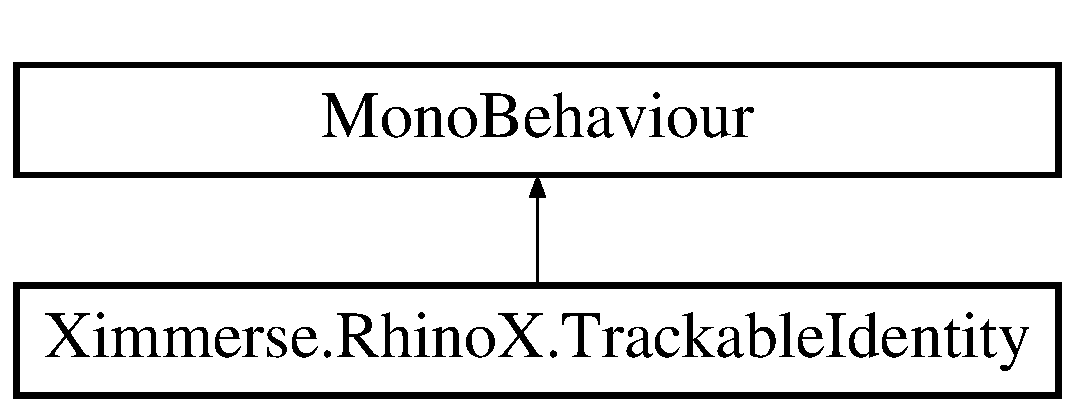
\includegraphics[height=2.000000cm]{class_ximmerse_1_1_rhino_x_1_1_trackable_identity}
\end{center}
\end{figure}
\subsection*{Public Attributes}
\begin{DoxyCompactItemize}
\item 
\mbox{\hyperlink{class_ximmerse_1_1_rhino_x_1_1_visiblity_change_event}{Visiblity\+Change\+Event}} \mbox{\hyperlink{class_ximmerse_1_1_rhino_x_1_1_trackable_identity_a586dc1b3013620e375e7887485b5ae13}{On\+Visibility\+Change}} = new \mbox{\hyperlink{class_ximmerse_1_1_rhino_x_1_1_visiblity_change_event}{Visiblity\+Change\+Event}}()
\begin{DoxyCompactList}\small\item\em Unity event \+: on object\textquotesingle{}s visibility change. \end{DoxyCompactList}\end{DoxyCompactItemize}
\subsection*{Properties}
\begin{DoxyCompactItemize}
\item 
int \mbox{\hyperlink{class_ximmerse_1_1_rhino_x_1_1_trackable_identity_a271412a107c63cfd093732698616f331}{Trackable\+ID}}\hspace{0.3cm}{\ttfamily  \mbox{[}get, set\mbox{]}}
\begin{DoxyCompactList}\small\item\em Gets or sets the trackable identifier. \end{DoxyCompactList}\item 
bool \mbox{\hyperlink{class_ximmerse_1_1_rhino_x_1_1_trackable_identity_a6265ce8a7d68c19fef42587c574a6981}{Is\+Visible}}\hspace{0.3cm}{\ttfamily  \mbox{[}get\mbox{]}}
\begin{DoxyCompactList}\small\item\em Is the marker visible at current frame ? \end{DoxyCompactList}\item 
\mbox{\Hypertarget{class_ximmerse_1_1_rhino_x_1_1_trackable_identity_ac5429b9063cf720fccfb564c1cfe58be}\label{class_ximmerse_1_1_rhino_x_1_1_trackable_identity_ac5429b9063cf720fccfb564c1cfe58be}} 
bool {\bfseries Debug\+View}\hspace{0.3cm}{\ttfamily  \mbox{[}get, set\mbox{]}}
\end{DoxyCompactItemize}


\subsection{Detailed Description}
Trackable object identity. Constraint by an integral trackable ID , represents a trackable object in real world. 



\subsection{Member Data Documentation}
\mbox{\Hypertarget{class_ximmerse_1_1_rhino_x_1_1_trackable_identity_a586dc1b3013620e375e7887485b5ae13}\label{class_ximmerse_1_1_rhino_x_1_1_trackable_identity_a586dc1b3013620e375e7887485b5ae13}} 
\index{Ximmerse\+::\+Rhino\+X\+::\+Trackable\+Identity@{Ximmerse\+::\+Rhino\+X\+::\+Trackable\+Identity}!On\+Visibility\+Change@{On\+Visibility\+Change}}
\index{On\+Visibility\+Change@{On\+Visibility\+Change}!Ximmerse\+::\+Rhino\+X\+::\+Trackable\+Identity@{Ximmerse\+::\+Rhino\+X\+::\+Trackable\+Identity}}
\subsubsection{\texorpdfstring{On\+Visibility\+Change}{OnVisibilityChange}}
{\footnotesize\ttfamily \mbox{\hyperlink{class_ximmerse_1_1_rhino_x_1_1_visiblity_change_event}{Visiblity\+Change\+Event}} Ximmerse.\+Rhino\+X.\+Trackable\+Identity.\+On\+Visibility\+Change = new \mbox{\hyperlink{class_ximmerse_1_1_rhino_x_1_1_visiblity_change_event}{Visiblity\+Change\+Event}}()}



Unity event \+: on object\textquotesingle{}s visibility change. 



\subsection{Property Documentation}
\mbox{\Hypertarget{class_ximmerse_1_1_rhino_x_1_1_trackable_identity_a6265ce8a7d68c19fef42587c574a6981}\label{class_ximmerse_1_1_rhino_x_1_1_trackable_identity_a6265ce8a7d68c19fef42587c574a6981}} 
\index{Ximmerse\+::\+Rhino\+X\+::\+Trackable\+Identity@{Ximmerse\+::\+Rhino\+X\+::\+Trackable\+Identity}!Is\+Visible@{Is\+Visible}}
\index{Is\+Visible@{Is\+Visible}!Ximmerse\+::\+Rhino\+X\+::\+Trackable\+Identity@{Ximmerse\+::\+Rhino\+X\+::\+Trackable\+Identity}}
\subsubsection{\texorpdfstring{Is\+Visible}{IsVisible}}
{\footnotesize\ttfamily bool Ximmerse.\+Rhino\+X.\+Trackable\+Identity.\+Is\+Visible\hspace{0.3cm}{\ttfamily [get]}}



Is the marker visible at current frame ? 

{\ttfamily true} if this instance is visible; otherwise, {\ttfamily false}.\mbox{\Hypertarget{class_ximmerse_1_1_rhino_x_1_1_trackable_identity_a271412a107c63cfd093732698616f331}\label{class_ximmerse_1_1_rhino_x_1_1_trackable_identity_a271412a107c63cfd093732698616f331}} 
\index{Ximmerse\+::\+Rhino\+X\+::\+Trackable\+Identity@{Ximmerse\+::\+Rhino\+X\+::\+Trackable\+Identity}!Trackable\+ID@{Trackable\+ID}}
\index{Trackable\+ID@{Trackable\+ID}!Ximmerse\+::\+Rhino\+X\+::\+Trackable\+Identity@{Ximmerse\+::\+Rhino\+X\+::\+Trackable\+Identity}}
\subsubsection{\texorpdfstring{Trackable\+ID}{TrackableID}}
{\footnotesize\ttfamily int Ximmerse.\+Rhino\+X.\+Trackable\+Identity.\+Trackable\+ID\hspace{0.3cm}{\ttfamily [get]}, {\ttfamily [set]}}



Gets or sets the trackable identifier. 

The trackable identifier.

The documentation for this class was generated from the following file\+:\begin{DoxyCompactItemize}
\item 
Trackable\+Identity.\+cs\end{DoxyCompactItemize}

\hypertarget{class_ximmerse_1_1_rhino_x_1_1_tracked_object_json}{}\section{Ximmerse.\+Rhino\+X.\+Tracked\+Object\+Json Class Reference}
\label{class_ximmerse_1_1_rhino_x_1_1_tracked_object_json}\index{Ximmerse.\+Rhino\+X.\+Tracked\+Object\+Json@{Ximmerse.\+Rhino\+X.\+Tracked\+Object\+Json}}


Tracked object json.  


\subsection*{Classes}
\begin{DoxyCompactItemize}
\item 
class \mbox{\hyperlink{class_ximmerse_1_1_rhino_x_1_1_tracked_object_json_1_1_card_group_json}{Card\+Group\+Json}}
\item 
class \mbox{\hyperlink{class_ximmerse_1_1_rhino_x_1_1_tracked_object_json_1_1_single_card_json}{Single\+Card\+Json}}
\end{DoxyCompactItemize}
\subsection*{Public Attributes}
\begin{DoxyCompactItemize}
\item 
\mbox{\Hypertarget{class_ximmerse_1_1_rhino_x_1_1_tracked_object_json_a2cff96b323cdee709f70857796362631}\label{class_ximmerse_1_1_rhino_x_1_1_tracked_object_json_a2cff96b323cdee709f70857796362631}} 
\mbox{\hyperlink{class_ximmerse_1_1_rhino_x_1_1_tracked_object_json_1_1_card_group_json}{Card\+Group\+Json}} {\bfseries C\+A\+R\+D\+\_\+\+G\+R\+O\+UP}
\item 
\mbox{\Hypertarget{class_ximmerse_1_1_rhino_x_1_1_tracked_object_json_aaaffeedb3f81e122cf331b59836d354a}\label{class_ximmerse_1_1_rhino_x_1_1_tracked_object_json_aaaffeedb3f81e122cf331b59836d354a}} 
\mbox{\hyperlink{class_ximmerse_1_1_rhino_x_1_1_tracked_object_json_1_1_single_card_json}{Single\+Card\+Json}} {\bfseries C\+A\+R\+D\+\_\+\+S\+I\+N\+G\+LE}
\end{DoxyCompactItemize}


\subsection{Detailed Description}
Tracked object json. 



The documentation for this class was generated from the following file\+:\begin{DoxyCompactItemize}
\item 
Tracked\+Object\+Json.\+cs\end{DoxyCompactItemize}

\hypertarget{class_ximmerse_1_1_rhino_x_1_1_object_tracking_profile_1_1_tracking_items}{}\section{Ximmerse.\+Rhino\+X.\+Object\+Tracking\+Profile.\+Tracking\+Items Class Reference}
\label{class_ximmerse_1_1_rhino_x_1_1_object_tracking_profile_1_1_tracking_items}\index{Ximmerse.\+Rhino\+X.\+Object\+Tracking\+Profile.\+Tracking\+Items@{Ximmerse.\+Rhino\+X.\+Object\+Tracking\+Profile.\+Tracking\+Items}}
\subsection*{Public Attributes}
\begin{DoxyCompactItemize}
\item 
Unity\+Engine.\+Object \mbox{\hyperlink{class_ximmerse_1_1_rhino_x_1_1_object_tracking_profile_1_1_tracking_items_aa0498b3e669a6a3089ae471647722664}{J\+S\+O\+N\+Config}} = null
\begin{DoxyCompactList}\small\item\em Editor only \end{DoxyCompactList}\item 
string \mbox{\hyperlink{class_ximmerse_1_1_rhino_x_1_1_object_tracking_profile_1_1_tracking_items_a4d4ed02f8829fbf3579876871920b1f7}{json\+Name}}
\begin{DoxyCompactList}\small\item\em The name of the json file. \end{DoxyCompactList}\item 
string \mbox{\hyperlink{class_ximmerse_1_1_rhino_x_1_1_object_tracking_profile_1_1_tracking_items_add856ff58e40c9650d63fed29e07e6e0}{json\+Content}}
\begin{DoxyCompactList}\small\item\em The content of the json. \end{DoxyCompactList}\end{DoxyCompactItemize}


\subsection{Member Data Documentation}
\mbox{\Hypertarget{class_ximmerse_1_1_rhino_x_1_1_object_tracking_profile_1_1_tracking_items_aa0498b3e669a6a3089ae471647722664}\label{class_ximmerse_1_1_rhino_x_1_1_object_tracking_profile_1_1_tracking_items_aa0498b3e669a6a3089ae471647722664}} 
\index{Ximmerse\+::\+Rhino\+X\+::\+Object\+Tracking\+Profile\+::\+Tracking\+Items@{Ximmerse\+::\+Rhino\+X\+::\+Object\+Tracking\+Profile\+::\+Tracking\+Items}!J\+S\+O\+N\+Config@{J\+S\+O\+N\+Config}}
\index{J\+S\+O\+N\+Config@{J\+S\+O\+N\+Config}!Ximmerse\+::\+Rhino\+X\+::\+Object\+Tracking\+Profile\+::\+Tracking\+Items@{Ximmerse\+::\+Rhino\+X\+::\+Object\+Tracking\+Profile\+::\+Tracking\+Items}}
\subsubsection{\texorpdfstring{J\+S\+O\+N\+Config}{JSONConfig}}
{\footnotesize\ttfamily Unity\+Engine.\+Object Ximmerse.\+Rhino\+X.\+Object\+Tracking\+Profile.\+Tracking\+Items.\+J\+S\+O\+N\+Config = null}



Editor only 

\mbox{\Hypertarget{class_ximmerse_1_1_rhino_x_1_1_object_tracking_profile_1_1_tracking_items_add856ff58e40c9650d63fed29e07e6e0}\label{class_ximmerse_1_1_rhino_x_1_1_object_tracking_profile_1_1_tracking_items_add856ff58e40c9650d63fed29e07e6e0}} 
\index{Ximmerse\+::\+Rhino\+X\+::\+Object\+Tracking\+Profile\+::\+Tracking\+Items@{Ximmerse\+::\+Rhino\+X\+::\+Object\+Tracking\+Profile\+::\+Tracking\+Items}!json\+Content@{json\+Content}}
\index{json\+Content@{json\+Content}!Ximmerse\+::\+Rhino\+X\+::\+Object\+Tracking\+Profile\+::\+Tracking\+Items@{Ximmerse\+::\+Rhino\+X\+::\+Object\+Tracking\+Profile\+::\+Tracking\+Items}}
\subsubsection{\texorpdfstring{json\+Content}{jsonContent}}
{\footnotesize\ttfamily string Ximmerse.\+Rhino\+X.\+Object\+Tracking\+Profile.\+Tracking\+Items.\+json\+Content}



The content of the json. 

\mbox{\Hypertarget{class_ximmerse_1_1_rhino_x_1_1_object_tracking_profile_1_1_tracking_items_a4d4ed02f8829fbf3579876871920b1f7}\label{class_ximmerse_1_1_rhino_x_1_1_object_tracking_profile_1_1_tracking_items_a4d4ed02f8829fbf3579876871920b1f7}} 
\index{Ximmerse\+::\+Rhino\+X\+::\+Object\+Tracking\+Profile\+::\+Tracking\+Items@{Ximmerse\+::\+Rhino\+X\+::\+Object\+Tracking\+Profile\+::\+Tracking\+Items}!json\+Name@{json\+Name}}
\index{json\+Name@{json\+Name}!Ximmerse\+::\+Rhino\+X\+::\+Object\+Tracking\+Profile\+::\+Tracking\+Items@{Ximmerse\+::\+Rhino\+X\+::\+Object\+Tracking\+Profile\+::\+Tracking\+Items}}
\subsubsection{\texorpdfstring{json\+Name}{jsonName}}
{\footnotesize\ttfamily string Ximmerse.\+Rhino\+X.\+Object\+Tracking\+Profile.\+Tracking\+Items.\+json\+Name}



The name of the json file. 



The documentation for this class was generated from the following file\+:\begin{DoxyCompactItemize}
\item 
Object\+Tracking\+Profile.\+cs\end{DoxyCompactItemize}

\hypertarget{class_ximmerse_1_1_rhino_x_1_1_triple_ground_plane}{}\section{Ximmerse.\+Rhino\+X.\+Triple\+Ground\+Plane Class Reference}
\label{class_ximmerse_1_1_rhino_x_1_1_triple_ground_plane}\index{Ximmerse.\+Rhino\+X.\+Triple\+Ground\+Plane@{Ximmerse.\+Rhino\+X.\+Triple\+Ground\+Plane}}


Tripple ground plane.  


Inheritance diagram for Ximmerse.\+Rhino\+X.\+Triple\+Ground\+Plane\+:\begin{figure}[H]
\begin{center}
\leavevmode
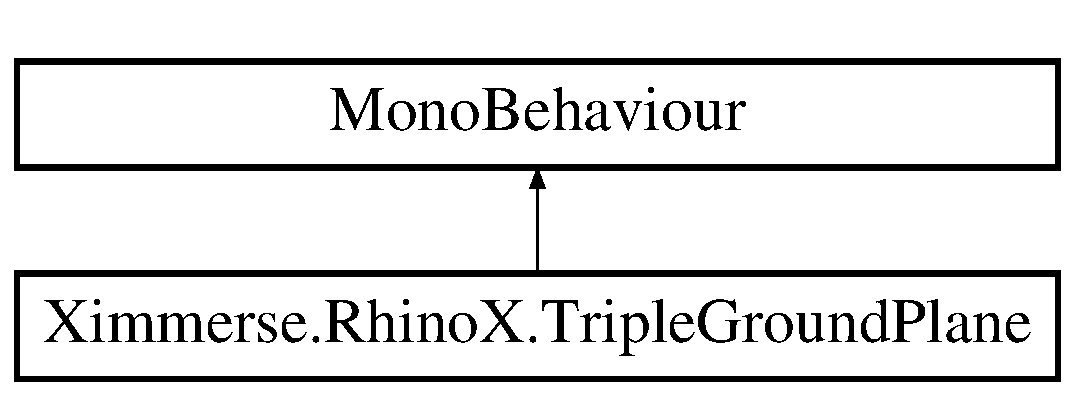
\includegraphics[height=2.000000cm]{class_ximmerse_1_1_rhino_x_1_1_triple_ground_plane}
\end{center}
\end{figure}


\subsection{Detailed Description}
Tripple ground plane. 



The documentation for this class was generated from the following file\+:\begin{DoxyCompactItemize}
\item 
H\+L\+A\+P\+I/\+Public/Triple\+Ground\+Plane.\+cs\end{DoxyCompactItemize}

\hypertarget{class_ximmerse_1_1_rhino_x_1_1_visiblity_change_event}{}\section{Ximmerse.\+Rhino\+X.\+Visiblity\+Change\+Event Class Reference}
\label{class_ximmerse_1_1_rhino_x_1_1_visiblity_change_event}\index{Ximmerse.\+Rhino\+X.\+Visiblity\+Change\+Event@{Ximmerse.\+Rhino\+X.\+Visiblity\+Change\+Event}}
Inheritance diagram for Ximmerse.\+Rhino\+X.\+Visiblity\+Change\+Event\+:\begin{figure}[H]
\begin{center}
\leavevmode
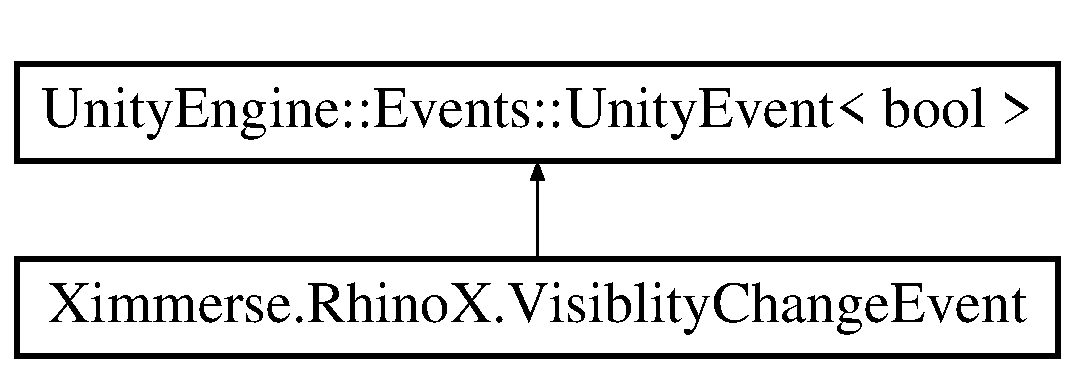
\includegraphics[height=2.000000cm]{class_ximmerse_1_1_rhino_x_1_1_visiblity_change_event}
\end{center}
\end{figure}


The documentation for this class was generated from the following file\+:\begin{DoxyCompactItemize}
\item 
Trackable\+Identity.\+cs\end{DoxyCompactItemize}

%--- End generated contents ---

% Index
\backmatter
\newpage
\phantomsection
\clearemptydoublepage
\addcontentsline{toc}{chapter}{Index}
\printindex

\end{document}
